\documentclass[12pt,a4paper,oneside]{report}

% ---------------------------------------------------------------------------
%  Student and project details (edit here; used throughout the front matter)
% ---------------------------------------------------------------------------
\newcommand{\ReportTitle}{VeriFact: Hallucination Detection in Large Language Model Outputs using Retrieval, Natural Language Inference and Conformal Prediction}
\newcommand{\ShortTitle}{Hallucination Detection using Retrieval, NLI and Conformal Prediction}
\newcommand{\StudentName}{Raj Majumder}
\newcommand{\RollNo}{23CH10050}
\newcommand{\Degree}{Bachelor of Technology (Hons.)}
\newcommand{\StudentDept}{Chemical Engineering}
\newcommand{\ProjectCourse}{B.Tech Project-I}
\newcommand{\Supervisor}{Professor Somesh Kumar}
\newcommand{\SupervisorDept}{Department of Mathematics}
\newcommand{\Semester}{Autumn Semester, 2026--27}
\newcommand{\SubmissionDate}{November 2026}

% ---------------------------------------------------------------------------
\usepackage[a4paper,left=1.25in,right=1in,top=1in,bottom=1in,headheight=15pt]{geometry}
\usepackage[T1]{fontenc}
\usepackage{lmodern}
\usepackage{amsmath,amssymb,amsthm,mathtools,bm}
\usepackage{graphicx}
\usepackage{booktabs,tabularx,multirow,array}
\usepackage{setspace}
\usepackage{fancyhdr}
\usepackage{titlesec}
\usepackage[font=small,labelfont=sc]{caption}
\usepackage{subcaption}
\usepackage{algorithm}
\usepackage[noend]{algpseudocode}
\usepackage{tikz}
\usetikzlibrary{arrows.meta,positioning,shapes.geometric,fit,calc}
\usepackage{enumitem}
\usepackage{xcolor}
\usepackage[numbers,sort&compress]{natbib}
\usepackage[hidelinks]{hyperref}
\usepackage{float}

\onehalfspacing
% Let floats sit with text instead of being deferred to sparse float-only pages
\renewcommand{\topfraction}{0.85}
\renewcommand{\bottomfraction}{0.7}
\renewcommand{\textfraction}{0.1}
\renewcommand{\floatpagefraction}{0.8}
\setcounter{topnumber}{3}
\setcounter{bottomnumber}{2}
\setcounter{totalnumber}{5}
\setlength{\parskip}{0.4em}
\graphicspath{{figures/}}

% Chapter headings in the style of the IIT Kharagpur thesis template
\titleformat{\chapter}[display]
  {\normalfont\huge}{\chaptertitlename\ \thechapter}{20pt}{\Huge}
\titlespacing*{\chapter}{0pt}{30pt}{40pt}

\pagestyle{fancy}
\fancyhf{}
\renewcommand{\chaptermark}[1]{\markboth{\chaptername\ \thechapter.\ \textit{#1}}{}}
\fancyhead[L]{\small\leftmark}
\fancyhead[R]{\small\thepage}
\renewcommand{\headrulewidth}{0.4pt}
\fancypagestyle{plain}{\fancyhf{}\fancyfoot[C]{\thepage}\renewcommand{\headrulewidth}{0pt}}

\theoremstyle{plain}
\newtheorem{theorem}{Theorem}[chapter]
\newtheorem{proposition}[theorem]{Proposition}
\newtheorem{lemma}[theorem]{Lemma}
\theoremstyle{definition}
\newtheorem{definition}[theorem]{Definition}
\theoremstyle{remark}
\newtheorem{remark}[theorem]{Remark}

\newcommand{\Con}{\textsc{Contradicted}}
\newcommand{\Unk}{\textsc{Unknown}}
\newcommand{\Sup}{\textsc{Supported}}
\newcommand{\Y}{\mathcal{Y}}
\newcommand{\E}{\mathbb{E}}
\newcommand{\Ind}{\mathbb{I}}
\newcommand{\code}[1]{\texttt{#1}}
\DeclareMathOperator*{\argmax}{arg\,max}

\begin{document}

% =========================== TITLE PAGE ====================================
\begin{titlepage}
\begin{center}
\vspace*{-1cm}
{\Large\bfseries \ReportTitle\par}
\vspace{0.8cm}
{\large \ProjectCourse{} report submitted to\\
Indian Institute of Technology Kharagpur\\
in partial fulfilment for the award of the degree of\\[0.2cm]
\textbf{\Degree}\\[0.2cm]
in\\[0.2cm]
\StudentDept\par}
\vspace{0.6cm}
{\large by\\[0.2cm]
\textbf{\StudentName}\\
(\RollNo)\par}
\vspace{0.6cm}
{\large Under the supervision of\\[0.2cm]
\textbf{\Supervisor}\\
\SupervisorDept\par}
\vspace{0.6cm}
\IfFileExists{figures/iitkgp_logo.png}{
\includegraphics[width=0.2\textwidth]{iitkgp_logo.png}}{}
\vfill
{\large Department of \StudentDept\\
Indian Institute of Technology Kharagpur\\
\Semester\\
\SubmissionDate\par}
\end{center}
\end{titlepage}

\pagenumbering{roman}
\setcounter{page}{1}

% =========================== DECLARATION ===================================
\chapter*{Declaration}
\addcontentsline{toc}{chapter}{Declaration}
\thispagestyle{plain}
I certify that
\begin{enumerate}[label=(\alph*),leftmargin=2em,itemsep=0.6em]
  \item The work contained in this report has been done by me under the guidance of my supervisor.
  \item The work has not been submitted to any other Institute for any degree or diploma.
  \item I have conformed to the norms and guidelines given in the Ethical Code of Conduct of the Institute.
  \item Whenever I have used materials (data, theoretical analysis, figures, and text) from other sources, I have given due credit to them by citing them in the text of the report and giving their details in the references. Further, I have taken permission from the copyright owners of the sources, whenever necessary.
\end{enumerate}
\vspace{3cm}
\noindent
\begin{tabular}{@{}l}
Date: \SubmissionDate\\
Place: Kharagpur
\end{tabular}
\hfill
\begin{tabular}{r@{}}
(\StudentName)\\
(\RollNo)
\end{tabular}

% =========================== CERTIFICATE ===================================
\clearpage
\thispagestyle{plain}
\addcontentsline{toc}{chapter}{Certificate}
\begin{center}
{\large DEPARTMENT OF MATHEMATICS\\
INDIAN INSTITUTE OF TECHNOLOGY KHARAGPUR\\
KHARAGPUR -- 721302, INDIA\par}
\vspace{0.8cm}
\IfFileExists{figures/iitkgp_logo.png}{
\includegraphics[width=0.2\textwidth]{iitkgp_logo.png}}{}\\[0.8cm]
{\Large\bfseries\itshape CERTIFICATE\par}
\end{center}
\vspace{0.6cm}
This is to certify that the project report entitled ``\textbf{\ReportTitle}'' submitted by \textbf{\StudentName} (Roll No.\ \RollNo) to Indian Institute of Technology Kharagpur towards partial fulfilment of requirements for the award of the degree of \Degree{} in \StudentDept{} is a record of bona fide work carried out by \StudentName{} under my supervision and guidance during the \Semester.
\vspace{3cm}

\noindent
\begin{tabular}{@{}l}
Date: \SubmissionDate\\
Place: Kharagpur
\end{tabular}
\hfill
\begin{tabular}{r@{}}
\textbf{\Supervisor}\\
\SupervisorDept\\
Indian Institute of Technology Kharagpur
\end{tabular}

% =========================== ABSTRACT ======================================
\chapter*{Abstract}
\addcontentsline{toc}{chapter}{Abstract}
\thispagestyle{plain}
\noindent\rule{\textwidth}{0.4pt}
\begin{tabular}{@{}ll}
Name of the student: & \textbf{\StudentName} \hfill Roll No: \textbf{\RollNo}\\
Degree for which submitted: & \textbf{\Degree}\\
Department: & \textbf{\StudentDept}\\
Thesis title: & \parbox[t]{0.6\textwidth}{\textbf{\ShortTitle}}\\
Thesis supervisor: & \textbf{\Supervisor}\\
Month and year of submission: & \textbf{\SubmissionDate}
\end{tabular}

\noindent\rule{\textwidth}{0.4pt}

Large language models (LLMs) produce fluent text that frequently contains \emph{hallucinations}: statements that are unsupported or contradicted by real-world evidence. This project designs, implements and statistically evaluates \textbf{VeriFact}, a system that checks a text for hallucinations claim by claim. The input is decomposed into atomic claims; for each claim, evidence is retrieved from Wikipedia, the open web and arXiv and ranked by a hybrid of dense sentence embeddings and BM25 combined through reciprocal rank fusion; a natural language inference (NLI) model (BART-large-MNLI) then scores every evidence snippet separately, and an asymmetric corroboration rule turns the per-snippet scores into a verdict. \textbf{Split conformal prediction} converts the NLI probabilities into prediction sets with a finite-sample coverage guarantee, and claims whose set is ambiguous are escalated, as a cascade, to a Wikidata knowledge graph and an LLM arbiter that argues for and against the claim before judging it.

The system was evaluated end to end, with live retrieval and LLM calls, on 300 claims each from \textbf{FEVER} and \textbf{FreshQA}. It reached an accuracy of \textbf{90.7\%} (Wilson 95\% CI [86.8\%, 93.5\%]; F1 0.91) on FEVER and \textbf{82.3\%} ([77.6\%, 86.2\%]; F1 0.85) on FreshQA, at a mean latency of 8.5\,s and 11.3\,s per claim. The NLI verdict alone settled 413 of the 600 claims, with 89\% accuracy, so the expensive stages ran only on the ambiguous remainder; on the claims it decided, the LLM arbiter fixed 60 NLI verdicts and broke 15 (exact McNemar test, $p = 1.6 \times 10^{-7}$). An exact ablation shows that every stage contributes significantly: the full pipeline gains 7.5 points of accuracy over the NLI verdict for 0.31 extra LLM calls per claim. Against a baseline that lets the LLM decide every claim, the cascade uses 35\% fewer LLM calls for an accuracy that is not significantly lower (88.2\% against 86.5\%, $p = 0.18$). The report places the statistical layer on a rigorous footing: it proves the conformal coverage guarantee, derives the Wilson score interval, the exact McNemar and Fisher tests, the Holm and Benjamini--Hochberg corrections and the power calculations used to compare results, removes the selection bias of a tuned decision parameter by cross-fitting, and calibrates the NLI probabilities by temperature scaling fitted by maximum likelihood, which halves the expected calibration error (11.4\% to 5.7\%) without changing any verdict. It also measures where the guarantees stop holding: on retrieved rather than gold evidence, conformal coverage falls to 83.2\%.

\vspace{0.5em}
\noindent\textbf{Keywords:} hallucination detection, fact verification, natural language inference, conformal prediction, calibration, hypothesis testing, retrieval-augmented verification, knowledge graphs.

% =========================== ACKNOWLEDGEMENTS ==============================
\chapter*{Acknowledgements}
\addcontentsline{toc}{chapter}{Acknowledgements}
\thispagestyle{plain}
I would like to sincerely thank my supervisor, \textbf{\Supervisor} of the \SupervisorDept{} at IIT Kharagpur, for the opportunity to work on this project and for the guidance given throughout it. The emphasis on statistical rigour in our discussions shaped the way the system was evaluated, and the feedback received greatly improved both the work and this report.

I am grateful to the Department of \StudentDept{} and the Department of Mathematics, IIT Kharagpur, for the academic environment and support that made this project possible. I also thank the maintainers of the open datasets, models and libraries on which this work builds, in particular FEVER, FreshQA, Wikipedia, Wikidata and the Hugging Face ecosystem. Finally, I thank my friends and family for their encouragement during the course of this work.

\vspace{2cm}
\hfill \StudentName

% =========================== CONTENTS ======================================
\clearpage
{\setlength{\parskip}{0pt}% list entries are paragraphs: no extra space between them
\tableofcontents
\clearpage
\addcontentsline{toc}{chapter}{List of Figures}
\listoffigures
\clearpage
\addcontentsline{toc}{chapter}{List of Tables}
\listoftables}

% =========================== ABBREVIATIONS =================================
\chapter*{Abbreviations}
\addcontentsline{toc}{chapter}{Abbreviations}
\thispagestyle{plain}
\begin{tabular}{@{}p{0.18\textwidth}p{0.75\textwidth}}
\textbf{AUROC} & Area Under the Receiver Operating Characteristic curve\\
\textbf{BART} & Bidirectional and Auto-Regressive Transformer\\
\textbf{BH} & Benjamini--Hochberg procedure\\
\textbf{BM25} & Best Matching 25 (Okapi ranking function)\\
\textbf{CI} & Confidence Interval\\
\textbf{ECE} & Expected Calibration Error\\
\textbf{FDR} & False Discovery Rate\\
\textbf{FEVER} & Fact Extraction and VERification benchmark\\
\textbf{FN / FP} & False Negative / False Positive\\
\textbf{FWER} & Family-Wise Error Rate\\
\textbf{IDF} & Inverse Document Frequency\\
\textbf{KG} & Knowledge Graph\\
\textbf{LLM} & Large Language Model\\
\textbf{MNLI} & Multi-Genre Natural Language Inference corpus\\
\textbf{NLI} & Natural Language Inference\\
\textbf{NLL} & Negative Log-Likelihood\\
\textbf{RRF} & Reciprocal Rank Fusion\\
\textbf{TN / TP} & True Negative / True Positive\\
\end{tabular}

\clearpage
\pagenumbering{arabic}
\setcounter{page}{1}

\chapter{Introduction}
\label{ch:intro}

\section{Motivation}

Large language models (LLMs) are now used to answer questions, summarise documents, draft reports and assist with research. Their output is fluent and confident regardless of whether it is correct, and a well-documented failure mode is \emph{hallucination}: the model states something that is not supported by, or is contradicted by, real-world evidence~\citep{ji2023survey,huang2023survey}. A hallucinated date, attribution or statistic is hard to spot precisely because it is embedded in otherwise plausible text, and its cost grows with the stakes of the application.

Checking an LLM answer by hand means splitting it into individual facts, searching for each one, reading the sources and judging whether they agree. This project automates that procedure. The resulting system, \textbf{VeriFact}, takes a text, typically an LLM answer, and returns a verdict for each atomic claim it contains (\Sup, \Con{} or \Unk), together with the evidence, the probabilities behind the verdict and a statistically grounded measure of how far that verdict can be trusted.

Two observations shape the design. First, verifying a claim with a large language model is accurate but slow and costly, whereas a small natural language inference (NLI) classifier is fast but makes characteristic mistakes. The system is therefore a \emph{cascade}: every claim passes through cheap deterministic stages, and only claims on which those stages are demonstrably uncertain are escalated to the expensive ones. Second, ``demonstrably uncertain'' must be made precise. The softmax output of a neural network is not a calibrated probability, so the decision to escalate is taken by \emph{split conformal prediction}, a distribution-free method from statistical learning theory that converts the classifier's output into a set of plausible labels with a finite-sample coverage guarantee~\citep{vovk2005algorithmic,angelopoulos2021gentle}.

Because the project was carried out under the Department of Mathematics, particular weight is given to the mathematical and statistical side of the work: the guarantees of the conformal layer are proved, every reported accuracy carries a correctly derived confidence interval, comparisons are made with exact hypothesis tests and corrected for multiple testing, and the limits of each guarantee are measured rather than assumed.

\section{Problem Statement}

Given an input text $T$, the detector must
\begin{enumerate}[itemsep=0.2em]
  \item split $T$ into atomic claims $c_1, \dots, c_n$, each expressing one checkable fact;
  \item for each claim $c$, retrieve an evidence set $\mathcal{E}(c) = \{e_1, \dots, e_k\}$ from external sources;
  \item assign a verdict $f(c, \mathcal{E}(c)) \in \Y = \{\Con, \Unk, \Sup\}$, where \Con{} marks a hallucination and \Unk{} is an abstention when the evidence is insufficient or genuinely conflicting;
\end{enumerate}
while keeping \emph{false accusations} (a true claim marked \Con) rare, keeping the number of LLM calls per claim low, and reporting the uncertainty of every verdict and every measured result honestly.

\section{Objectives}

The objectives of the project were:
\begin{enumerate}[itemsep=0.2em]
  \item To build an end-to-end hallucination detection pipeline that decomposes text into atomic claims, retrieves evidence from Wikipedia, the web and arXiv, and verifies each claim against that evidence.
  \item To combine dense and lexical retrieval signals in a principled way (BM25, sentence embeddings and reciprocal rank fusion) so that the most relevant evidence reaches the verifier.
  \item To design a decision rule over per-snippet NLI scores that reflects the measured, asymmetric reliability of support and contradiction.
  \item To use split conformal prediction as a statistically calibrated trigger for escalating uncertain claims to a knowledge graph and an LLM arbiter, and to measure how well its guarantee holds in deployment.
  \item To evaluate the full system on two public benchmarks, FEVER and FreshQA, with rigorous statistics: Wilson confidence intervals, exact hypothesis tests, multiple-comparison corrections, power analysis, cross-fitting and probability calibration.
  \item To provide an interactive web interface that exposes every intermediate computation, so that each verdict can be inspected step by step.
\end{enumerate}

\section{Contributions}

The main contributions of this work are:
\begin{itemize}[itemsep=0.2em]
  \item A cascaded verification pipeline in which 413 of 600 benchmark claims are settled by the NLI verdict alone (with 89\% accuracy), and LLM calls are spent only on the remaining ambiguous claims, at about 1.25 LLM calls per claim on average.
  \item An asymmetric \emph{corroboration rule} for NLI contradictions, derived from measured data: a lone contradicting snippet is wrong 29\% of the time and two agreeing snippets 11\% of the time, so a contradiction is accepted directly only when it is corroborated. Its parameter is validated by cross-fitting, which bounds the resulting optimism at about 0.3 percentage points.
  \item A complete treatment of split conformal prediction in this setting, including the proof of the coverage guarantee, conformal $p$-values, and an empirical measurement showing that coverage on retrieved evidence (83.2\%) falls below the nominal 90\% because exchangeability with the gold-evidence calibration set does not hold. A comparison with class-conditional (Mondrian) conformal prediction and adaptive prediction sets shows that the shortfall is shared by false and true claims and is not removed by changing the procedure.
  \item A statistically rigorous evaluation on 600 claims with live retrieval: accuracy 90.7\% on FEVER and 82.3\% on FreshQA, with the significance of every comparison established by exact tests and corrected for the eight tests reported.
  \item An exact ablation study, reconstructed from the computation traces without new model runs, showing that every stage of the cascade contributes significantly; a comparison with an LLM-only baseline, which the cascade matches within the statistical resolution of the benchmark while making 35\% fewer LLM calls; and a risk--coverage analysis of selective prediction.
  \item Temperature scaling of the NLI probabilities, fitted by Newton's method on a convex likelihood, which halves the expected calibration error without changing any decision.
  \item A web application that streams each claim's progress through the pipeline and shows its full computation trace, including a live demonstration of the conformal coverage argument.
\end{itemize}

\section{Organisation of the Report}

Chapter~\ref{ch:lit} reviews the literature on hallucination, fact verification, retrieval, natural language inference, conformal prediction and calibration. Chapter~\ref{ch:formulation} formalises the problem and gives an overview of the cascade. Chapter~\ref{ch:method} describes each stage of the pipeline with its algorithm and mathematics. Chapter~\ref{ch:stats} develops the statistical framework: conformal prediction, interval estimation, hypothesis testing, multiple comparisons, cross-fitting, power and calibration. Chapter~\ref{ch:impl} covers the implementation and the user interface. Chapter~\ref{ch:results} presents the evaluation protocol, the results and an analysis of the errors. Chapter~\ref{ch:conclusion} summarises the work, its limitations and directions for future work.

\chapter{Literature Review}
\label{ch:lit}

This chapter summarises the work on which the project builds: the study of hallucination in language models, automated fact verification, information retrieval, natural language inference, distribution-free uncertainty quantification, probability calibration, and LLM-based judgement.

\section{Hallucination in Large Language Models}

Surveys by \citet{ji2023survey} and \citet{huang2023survey} distinguish \emph{intrinsic} hallucinations, which contradict the source or prompt, from \emph{extrinsic} ones, which cannot be verified from the source and may be false in the world. For open-ended LLM answers the relevant notion is factuality: whether each statement agrees with real-world knowledge. Detection approaches fall into three families. \emph{Self-consistency} methods sample several answers and flag statements on which the samples disagree; they need no external data but cannot detect a hallucination the model repeats consistently. \emph{Model-internal} methods inspect token probabilities or hidden states, which requires access to the model. \emph{Retrieval-based} methods check each statement against external evidence. This project follows the third family, which works with any model, including closed ones accessed through an API, and produces evidence a user can read.

A recurring step in retrieval-based checking is to decompose a long answer into atomic facts before verifying them, so that each verdict concerns a single proposition; FActScore~\citep{min2023factscore} popularised this for evaluating the factual precision of long-form generation.

\section{Automated Fact Verification}

The FEVER shared task~\citep{thorne2018fever} framed fact verification as a three-way classification of a claim into \textsc{Supports}, \textsc{Refutes} or \textsc{Not Enough Info} against Wikipedia, with a pipeline of document retrieval, sentence selection and claim verification. Its 185{,}445 claims were written by annotators who altered sentences from Wikipedia, which makes it a clean benchmark for encyclopedic facts that do not change over time. FreshQA~\citep{vu2023freshllms} targets the opposite regime: questions whose answers change over time and questions with false premises, with answers maintained by its authors. Together they test stable encyclopedic knowledge and temporally sensitive, open-web knowledge.

\section{Information Retrieval}

\paragraph{Lexical retrieval.} The Okapi BM25 ranking function~\citep{robertson2009bm25} scores a document by the inverse document frequency of the query terms it contains, with saturation in term frequency and normalisation for document length. It remains a strong baseline for exact names, numbers and rare words.

\paragraph{Dense retrieval.} Sentence-BERT~\citep{reimers2019sbert} fine-tunes a Transformer encoder in a siamese setup so that the cosine similarity of pooled embeddings reflects semantic similarity. Small models such as \code{all-MiniLM-L6-v2} make dense similarity cheap enough to compute over hundreds of candidate paragraphs per query, and they recognise paraphrases that share no words with the query.

\paragraph{Rank fusion.} Lexical and dense scores live on incomparable scales. Reciprocal rank fusion (RRF)~\citep{cormack2009rrf} combines rankings rather than scores, summing $1/(\kappa + r)$ over the systems, and was shown to outperform more complex learned fusion methods.

\section{Natural Language Inference}

Natural language inference asks whether a premise entails, contradicts or is neutral towards a hypothesis. The Multi-Genre NLI corpus~\citep{williams2018mnli} provides about 433{,}000 annotated sentence pairs across genres. BART~\citep{lewis2020bart}, a denoising sequence-to-sequence Transformer, fine-tuned on MNLI (\code{facebook/bart-large-mnli}) is a widely used zero-shot verifier: with the evidence as premise and the claim as hypothesis, entailment, neutrality and contradiction map directly onto \Sup, \Unk{} and \Con. NLI models are known to rely on annotation artefacts; for instance, a premise describing a different situation is often read as contradicting the hypothesis, a behaviour this project measures and corrects for (Section~\ref{sec:nli}).

\section{Conformal Prediction}

Conformal prediction~\citep{vovk2005algorithmic} turns the output of any predictive model into prediction \emph{sets} that contain the true label with a user-chosen probability $1-\alpha$, under the sole assumption that the data are exchangeable. The \emph{split} (inductive) variant calibrates a single threshold on a held-out set, which makes it computationally trivial at prediction time. \citet{angelopoulos2021gentle} give an accessible account and discuss the marginal nature of the guarantee, its sensitivity to distribution shift, and the use of set size as a measure of uncertainty. In this project the set size serves as the escalation trigger of the cascade.

\section{Probability Calibration}

A classifier is calibrated when its stated confidence matches its frequency of being right. \citet{guo2017calibration} showed that modern neural networks are systematically over-confident and that \emph{temperature scaling}, dividing the logits by a single scalar fitted by maximum likelihood, is a remarkably effective fix. \citet{platt1999probabilistic} proposed fitting a logistic function to classifier scores. Calibration is measured by proper scoring rules such as the negative log-likelihood and the Brier score~\citep{brier1950verification}, and by the expected calibration error~\citep{naeini2015obtaining}.

\section{Statistical Evaluation of Classifiers}

Reporting an accuracy without its uncertainty invites over-interpretation of small differences. \citet{brown2001interval} showed that the textbook normal-approximation interval for a binomial proportion has poor coverage and recommended the Wilson score interval~\citep{wilson1927probable}. Paired comparisons of two classifiers on the same items are made with McNemar's test~\citep{mcnemar1947note}; independent proportions with the two-proportion $z$-test, Fisher's exact test~\citep{fisher1922interpretation} and Newcombe's interval for the difference~\citep{newcombe1998interval}. When several tests are reported, Holm's procedure~\citep{holm1979simple} controls the family-wise error rate and the Benjamini--Hochberg procedure~\citep{benjamini1995controlling} the false discovery rate. \citet{varma2006bias} documented the optimistic bias that arises when a parameter is tuned and evaluated on the same data, which cross-fitting removes.

\section{LLMs as Judges and Multi-Agent Debate}

LLMs can reason over paraphrase, multi-sentence evidence and dates, which NLI classifiers cannot. \citet{du2023improving} and \citet{liang2023encouraging} showed that letting several LLM agents argue opposing positions before a judgement improves factuality and reduces the tendency of a model to anchor on its first answer. This project adapts the idea into a single-call ``dialectical'' prompt with a defence, a prosecution and a judgement, and keeps a three-agent variant for ablation.

\section{Knowledge Graphs}

Wikidata is a collaboratively edited knowledge graph in which every fact is a typed statement (entity, property, value) with references. Many claims turn on a fact that a knowledge graph records exactly but that an NLI model reads poorly from prose, such as a date of birth, an award or the type of an entity. Structured statements are therefore a natural complement to retrieved passages for the hardest claims.

\section{Research Gap}

Existing retrieval-based checkers either trust a single verifier's output or call an LLM for every claim. The first is cheap but inherits the verifier's systematic errors; the second is accurate but slow and expensive. Few systems decide \emph{when} to escalate on statistical grounds, and fewer still measure whether the statistical guarantee they rely on actually holds on the evidence they retrieve. This project addresses that gap with a cascade whose routing is driven by conformal prediction, whose decision rules are derived from measured error rates, and whose evaluation reports every result with its uncertainty.

\chapter{Problem Formulation and System Overview}
\label{ch:formulation}

\section{Formal Task Definition}

A \emph{hallucination} is a statement produced by a language model that is not supported by, or is contradicted by, real-world evidence. Let $T$ be an input text. The detector computes
\begin{equation}
  T \;\longmapsto\; \bigl( c_i,\; \mathcal{E}(c_i),\; \hat{y}_i,\; \hat{\bm{\pi}}_i,\; \mathcal{C}_i \bigr)_{i=1}^{n},
\end{equation}
where $c_1, \dots, c_n$ are the atomic claims of $T$, $\mathcal{E}(c_i)$ the retrieved evidence, $\hat{y}_i \in \Y = \{\Con, \Unk, \Sup\}$ the verdict, $\hat{\bm{\pi}}_i \in \Delta^2$ (the probability simplex over $\Y$) the probability vector behind it, and $\mathcal{C}_i \subseteq \Y$ its conformal prediction set. \Con{} means the claim is a hallucination, \Sup{} that the evidence confirms it, and \Unk{} that the detector abstains.

\paragraph{Asymmetric costs.} The two errors are not equally harmful. A \emph{false accusation} (a true claim marked \Con) undermines the user's trust in correct answers and in the detector itself, whereas a missed hallucination leaves the user no worse off than without the detector. Abstention (\Unk) is preferable to a confident wrong verdict. These preferences are reflected in the decision rules of Chapter~\ref{ch:method}.

\paragraph{Answer-level verdict.} When an answer contains several claims, one contradicted claim makes the whole answer a hallucination:
\begin{equation}
  \hat{y}(T) = \begin{cases}
    \Con & \text{if } \exists\, i : \hat{y}_i = \Con, \\
    \Unk & \text{else if } \exists\, i : \hat{y}_i = \Unk, \\
    \Sup & \text{otherwise.}
  \end{cases}
\end{equation}
The summary report also gives the \emph{hallucination rate} $\frac{1}{n} \sum_{i} \Ind(\hat{y}_i = \Con)$.

\section{Notation}

Table~\ref{tab:notation} collects the symbols used in the rest of the report.

\begin{table}[H]
\centering
\caption{Notation used in the report.}
\label{tab:notation}
\small
\begin{tabular}{@{}ll@{}}
\toprule
Symbol & Meaning \\
\midrule
$c$ & an atomic claim \\
$e_i$, $\mathcal{E}$ & the $i$-th evidence snippet; the set of snippets for a claim \\
$\Y$ & the label set $\{\Con, \Unk, \Sup\}$ \\
$\mathbf{z} \in \mathbb{R}^3$ & NLI logits \\
$\hat{\pi}_y(e)$ & NLI probability of label $y$ with snippet $e$ as premise and $c$ as hypothesis \\
$\mathbf{c}, \mathbf{e}$ & sentence embeddings of a claim and a paragraph \\
$\tau$ & decisiveness threshold for a snippet ($0.80$) \\
$m$ & number of agreeing contradicting snippets needed to accept a contradiction ($2$) \\
$\mathcal{C}(X)$ & conformal prediction set for input $X$ \\
$\alpha$, $\hat{q}_\alpha$ & conformal significance level; calibrated conformal quantile \\
$T$ & temperature of the calibrated probabilities (also the input text, by context) \\
$\Ind(\cdot)$ & indicator function \\
\bottomrule
\end{tabular}
\end{table}

\section{Design Principle: a Statistically Routed Cascade}

Let $\text{cost}(\cdot)$ denote the time and API cost of a stage. NLI scoring of three snippets costs a fraction of a second on a laptop GPU; an LLM arbitration call costs one to three seconds and a unit of a limited API quota. If $\rho$ is the fraction of claims escalated, the expected cost per claim is
\begin{equation}
  \E[\text{cost}] = \text{cost}(\text{retrieval} + \text{NLI}) + \rho \cdot \text{cost}(\text{KG} + \text{LLM}),
\end{equation}
so the cascade is worthwhile when $\rho$ is small \emph{and} the claims escalated are those on which NLI is actually unreliable. The second condition is the hard part. Escalating on a hand-picked confidence threshold has no guarantee, because the NLI probabilities are not calibrated (Section~\ref{sec:calibration}). Escalation is instead triggered by the size of a split conformal prediction set (Section~\ref{sec:conformal}), which has a provable coverage property under exchangeability. Section~\ref{sec:routing-results} shows that the claims kept on the fast path are right 89\% of the time.

A single detector configuration serves every input: the web server and every benchmark construct the detector with the same defaults, and no setting depends on the dataset being evaluated.

\section{Pipeline Overview}

Figure~\ref{fig:pipeline} shows the stages and the routing between them. Each claim is processed independently, and the claims of one input are verified concurrently.

\begin{figure}[htbp]
\centering
\begin{tikzpicture}[
  node distance=0.45cm and 0.6cm,
  box/.style={draw, rounded corners=2pt, minimum width=4.6cm, minimum height=0.75cm, align=center, font=\small, fill=blue!4},
  dec/.style={draw, diamond, aspect=2.6, inner sep=1pt, align=center, font=\scriptsize, fill=orange!8},
  outbox/.style={draw, rounded corners=2pt, minimum width=2.6cm, minimum height=0.75cm, align=center, font=\scriptsize, fill=green!6},
  arr/.style={-{Stealth[length=2mm]}, thick}
]
\node[box] (in) {Input text $T$};
\node[box, below=of in] (dec) {Claim decomposition (\ref{sec:decomp})};
\node[box, below=of dec] (qg) {Query generation (\ref{sec:querygen})};
\node[box, below=of qg] (ret) {Evidence retrieval + hybrid re-ranking\\(\ref{sec:retrieval}--\ref{sec:rerank})};
\node[box, below=of ret] (nli) {NLI evidence scoring (\ref{sec:nli})};
\node[box, below=of nli] (cp) {Conformal prediction set (\ref{sec:conformal-stage})};
\node[dec, below=0.55cm of cp] (route) {Routing\\(\ref{sec:routing})};
\node[outbox, below=1.5cm of route, xshift=-4.2cm] (stand) {NLI verdict\\stands};
\node[outbox, below=1.5cm of route] (review) {Lightweight\\LLM review};
\node[outbox, below=1.5cm of route, xshift=4.2cm] (esc) {Wikidata KG (\ref{sec:kg})\\+ LLM arbiter (\ref{sec:arbiter})};
\node[box, below=1.0cm of review] (rep) {Verdict, evidence, report and UI};

\draw[arr] (in) -- (dec);
\draw[arr] (dec) -- node[right, font=\scriptsize]{claims $c_1, \dots, c_n$} (qg);
\draw[arr] (qg) -- (ret);
\draw[arr] (ret) -- (nli);
\draw[arr] (nli) -- (cp);
\draw[arr] (cp) -- (route);
\draw[arr] (route.west) -| node[pos=0.3, above, font=\scriptsize]{singleton set} (stand.north);
\draw[arr] (route) -- node[right, font=\scriptsize, align=left]{lone or contested\\contradiction} (review);
\draw[arr] (route.east) -| node[pos=0.3, above, font=\scriptsize]{ambiguous set} (esc.north);
\draw[arr] (stand.south) |- (rep.west);
\draw[arr] (review) -- (rep);
\draw[arr] (esc.south) |- (rep.east);
\draw[arr, dashed] (cp.east) -- ++(1.6,0) |- node[pos=0.25, right, font=\scriptsize, align=left]{\Unk{} or no evidence\\on first pass:\\query rewrite (once)} (qg.east);
\end{tikzpicture}
\caption{The VeriFact cascade. Cheap deterministic stages run on every claim; the conformal set decides which claims go to the expensive stages.}
\label{fig:pipeline}
\end{figure}

\chapter{Methodology}
\label{ch:method}

This chapter describes each stage of the pipeline: its purpose, the algorithm it runs and the mathematics behind it, illustrated with examples from real runs of the system. The statistical theory of the conformal layer is developed separately in Chapter~\ref{ch:stats}.

% --------------------------------------------------------------------------
\section{Claim Decomposition}
\label{sec:decomp}

A single sentence often bundles several facts, some true and some false: \emph{``Tim Cook replaced Steve Jobs in 2011 and founded Apple''} is half right. Verifying the sentence as a whole would force one verdict onto two facts. Decomposition splits the input into \emph{atomic claims}, each with exactly one checkable proposition.

\paragraph{Algorithm.}
\begin{enumerate}[itemsep=0.2em]
  \item \textbf{Atomic fast path.} If $T$ is a single sentence of at most 15 words and contains none of a conservative list of clause markers (\code{;}, \code{,}, \emph{and}, \emph{but}, \emph{which}, \emph{because}, \emph{who}, \emph{that}, \emph{with}, \dots), it is already atomic and is returned unchanged, with no LLM call.
  \item \textbf{LLM decomposition.} Otherwise an LLM returns a JSON array of atomic facts under two mandatory rules. \emph{Coreference resolution}: every pronoun and implicit reference is replaced by the explicit proper noun, so each claim can be verified on its own. \emph{Polarity preservation}: the truth value and negations of the original text are kept verbatim, and the model must never ``correct'' a false statement into a true one, which would silently delete the hallucination the detector is meant to find.
  \item \textbf{Fallback.} If the LLM call fails or returns invalid JSON, the text is split into sentences with the NLTK tokenizer.
\end{enumerate}

\begin{table}[htbp]
\centering
\caption{Claim decomposition examples.}
\label{tab:decomp}
\small
\begin{tabularx}{\textwidth}{@{}XlX@{}}
\toprule
Input & Route & Output claims \\
\midrule
\emph{Juneau is the capital of Alaska.} & fast path & \emph{Juneau is the capital of Alaska.} \\
\emph{Albert Einstein was born in 1950 in San Francisco, and he won the Nobel Prize in Literature in 1980.} & LLM & \emph{Albert Einstein was born in 1950.}; \emph{Albert Einstein was born in San Francisco.}; \emph{Albert Einstein won the Nobel Prize in Literature in 1980.} \\
\bottomrule
\end{tabularx}
\end{table}

% --------------------------------------------------------------------------
\section{Query Generation}
\label{sec:querygen}

Searching for the whole claim string returns noisy results; searching for the \emph{entities} the claim is about retrieves the encyclopedia articles that contain the deciding fact. This stage maps a claim to at most three queries, a domain (\emph{general} or \emph{scientific}) and a flag saying whether the claim depends on the present date.

A \textbf{fast path} handles short claims without ambiguous pronouns by regular expressions over common relational patterns (\emph{is the co-founder of}, \emph{was born in}, \emph{was directed by}, \emph{is a}, \dots): the subject and the capitalised object become the queries. Claims about creative works (\emph{album}, \emph{film}, \emph{series}, \dots) and claims using epithets (\emph{``the father of''}) are excluded, because they need disambiguation. Otherwise an \textbf{LLM path} is used, instructed to disambiguate titles (e.g.\ \emph{``Pixels (2015 film)''}), to resolve implicit references and to flag claims about the present. For temporal claims the evidence text is later prefixed with the current date, so that the arbiter can reason about recency.

\begin{table}[htbp]
\centering
\caption{Query generation examples.}
\label{tab:queries}
\small
\begin{tabularx}{\textwidth}{@{}XlX@{}}
\toprule
Claim & Route & Queries \\
\midrule
\emph{Barack Obama was born in Hawaii.} & fast path & \code{["Barack Obama", "Hawaii"]} \\
\emph{Bones is a television series.} & LLM (creative work) & \code{["Bones (TV series)"]} \\
\emph{The 8th president of the United States is buried in Kinderhook, New York.} & LLM & \code{["Martin Van Buren", "Kinderhook (town) New York"]} \\
\bottomrule
\end{tabularx}
\end{table}

% --------------------------------------------------------------------------
\section{Evidence Retrieval}
\label{sec:retrieval}

Evidence is collected from complementary sources, all fetched concurrently:
\begin{itemize}[itemsep=0.2em]
  \item \textbf{Wikipedia} (per query): the top two search results, with auto-suggestion disabled (it silently replaces titles), disambiguation pages resolved to their first option, and reference sections removed.
  \item \textbf{arXiv} (scientific claims only): up to three abstracts per query.
  \item \textbf{Web search} (once per claim, on the full claim text): six search engines are queried in parallel and the first to answer is used, with at most three results, capped at 5\,s so that a blocked engine can never stall the pipeline.
\end{itemize}

\paragraph{Chunking.} Wikipedia text is split into sentences and grouped into overlapping windows of five sentences with stride three. Window $j$ covers sentences $3j+1, \dots, 3j+5$, so consecutive windows share two sentences, and any fact stated across two adjacent sentences is contained whole in some window. Each window is one candidate paragraph.

\paragraph{Claim-echo filtering.} A web search for the exact claim frequently returns pages that merely quote it, including fact-checks that quote a false claim before debunking it. An NLI model reads a verbatim quote as perfect entailment, so a false claim could ``support itself''. Let $W(x)$ be the set of lower-cased word tokens of a text $x$. A sentence $s$ of a web snippet is removed if
\begin{equation}
  \frac{\lvert W(c) \cap W(s) \rvert}{\lvert W(c) \rvert} \ge 0.8,
\end{equation}
and a snippet left with fewer than eight tokens is dropped. Encyclopedic text is never filtered, since a Wikipedia sentence that closely matches a claim is genuine support, not an echo. In the evaluation the filter removed at least one web snippet for 37 of the 600 claims.

% --------------------------------------------------------------------------
\section{Hybrid Re-Ranking}
\label{sec:rerank}

A query typically returns dozens of candidate paragraphs; only the $k = 3$ most relevant are passed to the NLI model. Two complementary relevance signals are combined.

\paragraph{Dense similarity.} Claim and paragraphs are embedded with \code{all-MiniLM-L6-v2}~\citep{reimers2019sbert}, a six-layer sentence Transformer producing 384-dimensional vectors. For token embeddings $\mathbf{h}_1, \dots, \mathbf{h}_L$ the sentence embedding is the normalised mean
\begin{equation}
  \bar{\mathbf{h}} = \frac{1}{L} \sum_{t=1}^{L} \mathbf{h}_t, \qquad \mathbf{e} = \frac{\bar{\mathbf{h}}}{\lVert \bar{\mathbf{h}} \rVert_2},
\end{equation}
and relevance is the cosine similarity, which for unit vectors is a dot product: $\operatorname{sim}(\mathbf{c}, \mathbf{e}) = \mathbf{c}^\top \mathbf{e} \in [-1, 1]$.

\paragraph{Sparse similarity (BM25).} For a claim with tokens $t_1, \dots, t_Q$ and $N$ candidate paragraphs, the Okapi BM25 score~\citep{robertson2009bm25} of paragraph $d$ is
\begin{equation}
  \operatorname{BM25}(d, c) = \sum_{j=1}^{Q} \operatorname{IDF}(t_j) \cdot \frac{f(t_j, d)\,(k_1 + 1)}{f(t_j, d) + k_1 \left( 1 - b + b\, \dfrac{\lvert d \rvert}{\text{avgdl}} \right)},
\end{equation}
\begin{equation}
  \operatorname{IDF}(t) = \ln \frac{N - n(t) + 0.5}{n(t) + 0.5},
\end{equation}
where $f(t, d)$ is the term frequency, $\lvert d \rvert$ the paragraph length, $\text{avgdl}$ the mean length, $n(t)$ the number of candidates containing $t$, $k_1 = 1.5$ and $b = 0.75$. The fraction is increasing and bounded in $f$, tending to $k_1 + 1$, so repeating a word has diminishing returns, and the factor in $\lvert d \rvert$ penalises long paragraphs. A term in more than half the candidates would receive a negative IDF; such values are replaced by a quarter of the mean IDF.

\paragraph{Reciprocal rank fusion.} Cosine similarity lies in $[-1,1]$ and BM25 is unbounded, so the two are combined through ranks. With $r_{\text{dense}}(d)$ and $r_{\text{bm25}}(d)$ the 1-based ranks,
\begin{equation}
  \operatorname{RRF}(d) = \frac{1}{\kappa + r_{\text{dense}}(d)} + \frac{1}{\kappa + r_{\text{bm25}}(d)}, \qquad \kappa = 60.
\end{equation}
Because $1/(\kappa + r)$ is convex and flat for large $\kappa$, a paragraph ranked well by \emph{both} signals beats one ranked first by only one of them. Paragraphs are then visited in decreasing RRF order and the first three that pass a relevance floor ($\operatorname{sim} \ge 0.20$ or $\operatorname{BM25} > 1.0$) are kept. If none qualifies, retrieval returns nothing rather than feeding unrelated text to the verifier.

\paragraph{Worked example.} For the FEVER claim \emph{``Bones is a cuisine''} (query \code{["Bones"]}), 68 unique candidates were retrieved. The top paragraph, a web result on \emph{``bone swimming cuisine''}, was second by dense similarity and first by BM25, so
\[
  \operatorname{RRF} = \frac{1}{60 + 2} + \frac{1}{60 + 1} = 0.016129 + 0.016393 = 0.032522.
\]
A Wikipedia paragraph on the femur, only eighth by dense similarity but second by BM25, entered the top three: fusion rewards agreement between the rankings.

% --------------------------------------------------------------------------
\section{NLI Evidence Scoring}
\label{sec:nli}

\paragraph{The model.} The verifier is \code{facebook/bart-large-mnli}: BART-large~\citep{lewis2020bart} (12 encoder and 12 decoder layers, hidden size 1{,}024, about 407M parameters) fine-tuned on MultiNLI~\citep{williams2018mnli}. The evidence is the premise and the claim the hypothesis. The final decoder state at the end-of-sequence token, $\mathbf{h}_{\text{eos}} \in \mathbb{R}^{1024}$, is mapped to three logits by a two-layer head,
\begin{equation}
  \mathbf{z} = \mathbf{W}_2 \tanh(\mathbf{W}_1 \mathbf{h}_{\text{eos}} + \mathbf{b}_1) + \mathbf{b}_2,
\end{equation}
which are normalised by softmax:
\begin{equation}
  \hat{\pi}_y = \frac{\exp(z_y)}{\sum_{y'} \exp(z_{y'})}, \qquad \hat{y} = \argmax_{y \in \Y} \hat{\pi}_y.
\end{equation}

\paragraph{Scoring snippets separately.} If all snippets are concatenated into one premise, the decisive sentence is surrounded by background text and decisive entailments collapse towards \emph{neutral} (\emph{context dilution}). Each snippet $e_i$ is therefore scored on its own, giving $\hat{\bm{\pi}}(e_i)$, and the judgements are combined in three steps. A snippet is \emph{decisive} for label $y$ when $\hat{\pi}_y(e_i) \ge \tau = 0.80$.

\paragraph{Step 1: source conflict.} With $S = \max_i \hat{\pi}_{\text{sup}}(e_i)$ and $K = \max_i \hat{\pi}_{\text{con}}(e_i)$, sources genuinely disagree when
\begin{equation}
  S \ge 0.85 \;\wedge\; K \ge 0.85 \;\wedge\; \lvert S - K \rvert < 0.12 .
\end{equation}
The verdict is then \Unk, and the arbiter is told that the sources conflict.

\paragraph{Step 2: the corroboration rule.} Support and contradiction are not equally reliable. MNLI-trained models often assign a confident contradiction to a snippet that is merely adjacent to the claim, because a premise describing a different situation was usually labelled a contradiction in training. On the 600 evaluation claims, the number of decisive contradicting snippets turned out to be the strongest available signal of whether a refutation is real (Table~\ref{tab:corroboration}, Figure~\ref{fig:corroboration}).

\begin{table}[htbp]
\centering
\caption{Reliability of NLI refutations by the number of decisive contradicting snippets (600 claims).}
\label{tab:corroboration}
\begin{tabular}{@{}lccc@{}}
\toprule
Decisive contradicting snippets & Claims & Claim actually false & Refutation wrong \\
\midrule
1 & 99 & 70 & 29\% \\
2 & 62 & 55 & 11\% \\
3 or more & 113 & 108 & 4\% \\
decisive support also present & 29 & 9 & 69\% \\
\bottomrule
\end{tabular}
\end{table}

\begin{figure}[htbp]
\centering
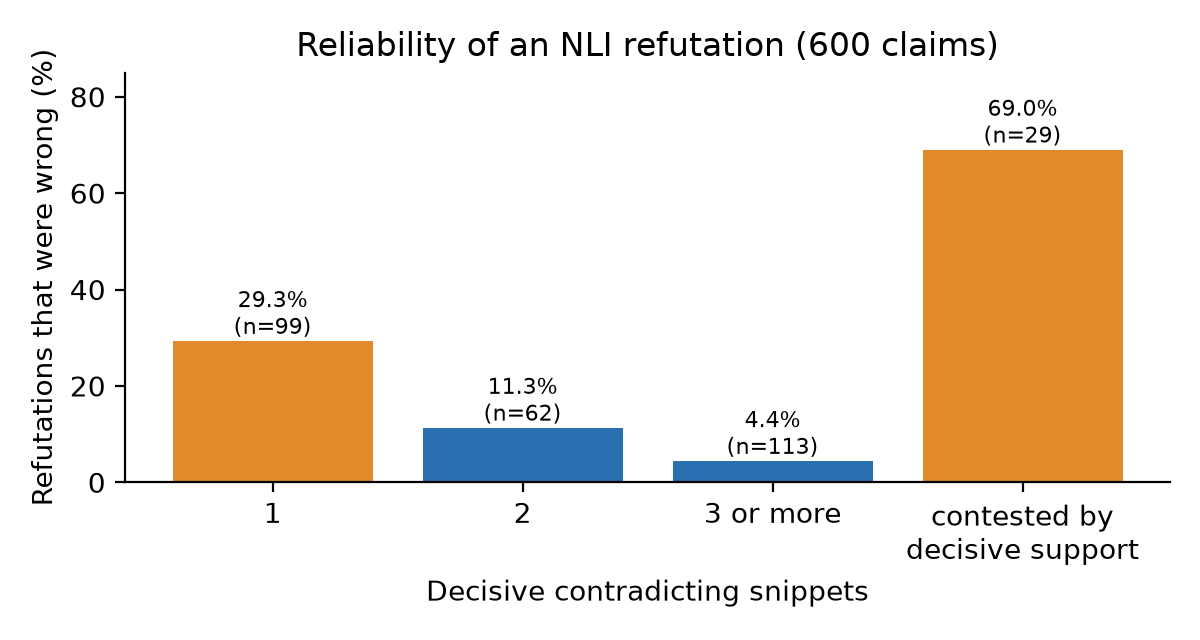
\includegraphics[width=0.72\textwidth]{corroboration.png}
\caption{Share of NLI refutations that were wrong, by the number of decisive contradicting snippets.}
\label{fig:corroboration}
\end{figure}

Let $D_{\text{sup}} = \{ i : \hat{y}(e_i) = \Sup,\ \hat{\pi}_{\text{sup}}(e_i) \ge \tau \}$ and $D_{\text{con}} = \{ i : \hat{y}(e_i) = \Con,\ \hat{\pi}_{\text{con}}(e_i) \ge \tau \}$. The verdict is
\begin{equation}
\label{eq:corroboration}
\hat{y} = \begin{cases}
\Sup & \text{if } \lvert D_{\text{sup}} \rvert \ge 1,\ D_{\text{con}} = \varnothing, \\
\Con & \text{if } \lvert D_{\text{con}} \rvert \ge m,\ D_{\text{sup}} = \varnothing,\ \text{no shared role}, \\
\text{LLM review} & \text{if } \lvert D_{\text{con}} \rvert \ge 1 \text{, otherwise}, \\
\text{Step 3} & \text{if } D_{\text{sup}} = D_{\text{con}} = \varnothing,
\end{cases}
\end{equation}
with $m = 2$. A lone or contested contradiction is thus passed to the LLM for review, while a corroborated one is accepted directly. A \emph{shared role} is a non-exclusive title (\emph{co-founder}, \emph{member}, \emph{actor}, \dots): MNLI models exhibit an exclusivity bias, reading ``$B$ co-founded $X$'' as contradicting ``$A$ co-founded $X$'', so such contradictions are never accepted directly. The choice $m = 2$ was read from Table~\ref{tab:corroboration}, which comes from the same claims on which accuracy is reported; Section~\ref{sec:crossfit} removes the resulting selection bias by cross-fitting.

\paragraph{Step 3: joint fallback.} If no snippet is decisive, the snippets are concatenated and scored once. This lets the model combine facts spread across snippets, the one case where concatenation helps.

\paragraph{Worked example.} For \emph{``Bones is a cuisine''} (gold label: false), the three snippets gave:
\begin{center}
\small
\begin{tabular}{@{}lcccl@{}}
\toprule
Snippet & $\hat{\pi}_{\text{con}}$ & $\hat{\pi}_{\text{unk}}$ & $\hat{\pi}_{\text{sup}}$ & Decisive? \\
\midrule
\emph{Bone swimming \dots} (web) & 0.2973 & 0.0717 & 0.6310 & no \\
\emph{A bone is a rigid \dots} (Wikipedia) & 0.9594 & 0.0388 & 0.0018 & yes (\Con) \\
\emph{The largest bone \dots} (Wikipedia) & 0.9934 & 0.0063 & 0.0003 & yes (\Con) \\
\bottomrule
\end{tabular}
\end{center}
$S = 0.631 < 0.85$, so there is no conflict; $\lvert D_{\text{con}} \rvert = 2 \ge m$ and $D_{\text{sup}} = \varnothing$, so the verdict is \Con{} with $\hat{\bm{\pi}} = (0.9934, 0.0063, 0.0003)$, without any LLM call.

% --------------------------------------------------------------------------
\section{Conformal Uncertainty Layer}
\label{sec:conformal-stage}

The probability vector of the verdict is passed to a split conformal predictor (theory in Section~\ref{sec:conformal}). With the production calibration ($n = 100$ FEVER claims, $\alpha = 0.10$, $\hat{q} = 0.8985$), a label enters the prediction set when its probability is at least $1 - \hat{q} = 0.1015$:
\begin{equation}
  \mathcal{C}(X) = \{ y \in \Y : \hat{\pi}_y(X) \ge 1 - \hat{q}_\alpha \}.
\end{equation}
For the \emph{Bones} example the set is the singleton $\{\Con\}$ and the verdict stands. A vector such as $(0.62, 0.30, 0.08)$ gives $\{\Con, \Unk\}$: the NLI posterior is spread over two labels, and the claim is escalated.

% --------------------------------------------------------------------------
\section{Routing: Query Rewrite, Absence Evaluation and Escalation}
\label{sec:routing}

\paragraph{Self-reflective query rewrite.} On the first pass only, if no evidence was found or the verdict is \Unk, an LLM receives the claim, the queries tried and the unhelpful evidence, diagnoses why the search failed and proposes up to two divergent queries. Retrieval and scoring run again; first-pass evidence is kept, so an empty second search cannot discard it.

\paragraph{Absence evaluation.} If evidence is still missing, absence is informative only for prominent facts: a major, widely recorded event that cannot be found is almost certainly false, whereas a minor detail may simply not be online. An LLM decides which case applies and returns \Con{} or \Unk.

\paragraph{Escalation rule.} A claim is fully escalated to the knowledge graph and the LLM arbiter when
\begin{equation}
\label{eq:escalate}
  \text{escalate}(X) \iff
  \begin{aligned}[t]
    & \hat{y} = \Unk \;\vee\; \lvert \mathcal{C}(X) \rvert > 1 \;\vee\; \Unk \in \mathcal{C}(X) \\
    & \vee\; (\text{shared} \wedge \hat{y} = \Con).
  \end{aligned}
\end{equation}
Here ``shared'' means the claim has a shared role. If it is not escalated but Step~2 flagged a lone or contested contradiction, it receives a \emph{lightweight review}: one LLM call over the evidence already retrieved. Otherwise the NLI verdict stands. Each result records which of these routes produced it.

% --------------------------------------------------------------------------
\section{Knowledge Graph Evidence from Wikidata}
\label{sec:kg}

Many escalated claims turn on a fact that Wikidata records exactly (a date, a place, an award, the type of an entity) and that an NLI model reads poorly from prose. For each claim the pipeline builds a small graph $G = (V, E)$ whose nodes are Wikidata entities and literal values and whose edges are statements, and gives the relevant statements to the arbiter as evidence. No LLM call is made.

\paragraph{Entity resolution.} Each entity named by query generation is resolved to a Wikidata item through the English Wikipedia page of that title; otherwise one search is made, and a result is accepted only if it shares a content word with the name. Names that do not resolve are left out rather than replaced by a near match.

\paragraph{Relation matching.} The claim's relation is matched to one of 77 common properties. Let $\mathbf{r}$ be the embedding of the claim without its subject's name, $\mathbf{r}'$ that of the claim without any entity name, and $T_p$ the label and phrasings of property $p$. Its score is
\begin{multline}
  s(p) = \max_{\mathbf{x} \in \{\mathbf{r}, \mathbf{r}'\}} \max_{\mathbf{t} \in T_p} \cos(\mathbf{x}, \mathbf{t}) + 0.12\,\Ind_{\text{date}}(c)\Ind_{\text{date}}(p) \\
  - 0.08\,\bigl(1 - \Ind_{\text{date}}(c)\bigr)\Ind_{\text{date}}(p) + 0.10\,\Ind_{\text{recorded}}(p),
\end{multline}
where $\Ind_{\text{date}}(c)$ indicates that the claim states a date, $\Ind_{\text{date}}(p)$ that $p$ is a date property, and $\Ind_{\text{recorded}}(p)$ that $p$ is recorded for an entity of the claim. The claim's property is $\argmax_p s(p)$ if its score is at least $0.45$. The claimed value is then compared with the recorded values, giving \emph{agrees}, \emph{differs}, \emph{not listed} or \emph{not identified}.

\paragraph{Example.} \emph{``The Crips are a band''} was escalated, and the arbiter received \emph{Crips --- instance of: gang}, \emph{inception: 1969}, \emph{headquarters location: Los Angeles}; it judged the claim \Con. For \emph{``Albert Einstein was born in 1950''} the statements include the recorded date of birth, \emph{14 March 1879}.

\paragraph{Coverage.} Of the 600 benchmark claims, 553 resolved to a Wikidata graph, built in a median of 1.6\,s. The lookup starts in a background thread as soon as the entities are known, alongside retrieval and NLI scoring, so it is usually ready by the time a claim escalates.

% --------------------------------------------------------------------------
\section{LLM Arbitration}
\label{sec:arbiter}

Escalated claims and lone or contested contradictions are decided by an LLM, which can handle paraphrase, implicit entailment, multi-sentence reasoning and dates. In the default \emph{dialectical} mode a single prompt makes the model write three sections before its verdict:
\begin{enumerate}[itemsep=0.2em]
  \item \textbf{Defence}: the strongest plausible case that the evidence supports the claim, quoting it;
  \item \textbf{Prosecution}: ungrounded assumptions, missing facts and direct contradictions;
  \item \textbf{Judgement}: weighing the two strictly against the raw evidence.
\end{enumerate}
Writing both opposing cases first counters the tendency of an autoregressive model to anchor on whichever argument it generates first~\citep{du2023improving,liang2023encouraging}. A three-agent variant, in which defence and prosecution run independently and a separate judge reads both, is kept for ablation studies.

The prompt also encodes decision rules: natural entailment is preferred over hyper-literal pedantry; a claimed award \emph{win} is contradicted by evidence of only a \emph{nomination}; and a claim that refers to an entity by a wrong name, title or date is \Con, so that the arbiter never silently repairs a false premise. \Unk{} is reserved for evidence that is absent, unrelated or genuinely balanced. If the LLM call itself fails, the result is flagged as an outage rather than reported as an abstention.

% --------------------------------------------------------------------------
\section{End-to-End Algorithm and Cost Model}
\label{sec:algorithm}

Algorithm~\ref{alg:verify} summarises the verification of one claim.

\paragraph{Cost model.} Decomposition, query generation, rewrite, absence evaluation, review and arbitration each cost zero or one LLM call; the Wikidata evidence costs none. A claim settled on the fast path with fast-path queries needs no LLM call at all. In the evaluation (Chapter~\ref{ch:results}) a claim cost 1.05 LLM calls on average on FEVER and 1.45 on FreshQA: 0.86 when the NLI verdict stood, 1.88 with a lightweight review and 2.32 with full escalation.

\begin{algorithm}[htbp]
\caption{Verification of a single claim $c$}
\label{alg:verify}
\begin{algorithmic}[1]
\State $(Q, \text{domain}, \text{temporal}) \gets \textsc{GenerateQueries}(c)$
\State $P \gets \varnothing$ \Comment{evidence pool across passes}
\For{$\text{pass} \in \{1, 2\}$}
  \State $E \gets \textsc{StripEchoes}(\textsc{Rerank}(\textsc{Retrieve}(Q, c, \text{domain}), c, k{=}3), c)$
  \State $P \gets P \cup E$; \textbf{if} $E = \varnothing$ \textbf{then} $E \gets P$
  \If{$E = \varnothing$}
    \If{$\text{pass} = 1$} $Q \gets \textsc{Rewrite}(c)$; \textbf{continue} \EndIf
    \State \Return $\textsc{AbsenceEval}(c)$
  \EndIf
  \State $(\hat{y}, \hat{\bm{\pi}}, \text{review}) \gets \textsc{Score}(c, E)$ \Comment{Section~\ref{sec:nli}}
  \State $\mathcal{C} \gets \{ y : \hat{\pi}_y \ge 1 - \hat{q} \}$ \Comment{Section~\ref{sec:conformal-stage}}
  \If{$\hat{y} = \Unk$ \textbf{and} $\text{pass} = 1$} $Q \gets \textsc{Rewrite}(c, E)$; \textbf{continue} \EndIf
  \If{$\textsc{Escalate}(\hat{y}, \mathcal{C})$} \Comment{rule~\eqref{eq:escalate}}
    \State \Return $\textsc{Arbitrate}(c, E \cup \textsc{WikidataEvidence}(c))$
  \ElsIf{review}
    \State \Return $\textsc{Arbitrate}(c, E)$
  \EndIf
  \State \Return $\hat{y}$
\EndFor
\end{algorithmic}
\end{algorithm}

\chapter{Statistical Framework}
\label{ch:stats}

This chapter develops the statistical tools on which the system and its evaluation rest: split conformal prediction, which drives the routing of claims; interval estimation and hypothesis tests, which are used to report and compare results; cross-fitting, which removes the bias of a tuned parameter; power analysis, which tells how many claims a conclusive comparison needs; and temperature scaling, which calibrates the NLI probabilities. Each method is stated with its assumptions and derived or proved.

% ==========================================================================
\section{Split Conformal Prediction}
\label{sec:conformal}

\subsection{Setting}

Let $(X_1, Y_1), \dots, (X_n, Y_n)$ be a \emph{calibration set} of labelled claims, never used for anything else, and $(X_{n+1}, Y_{n+1})$ a new claim whose label is unknown. The NLI model gives a probability vector $\hat{\bm{\pi}}(X)$ over $\Y$.

\begin{definition}[Exchangeability]
Random variables $Z_1, \dots, Z_{n+1}$ are \emph{exchangeable} if for every permutation $\sigma$ of $\{1, \dots, n+1\}$ the vector $(Z_{\sigma(1)}, \dots, Z_{\sigma(n+1)})$ has the same joint distribution as $(Z_1, \dots, Z_{n+1})$.
\end{definition}

Independent and identically distributed variables are exchangeable; the converse need not hold.

\begin{definition}[Non-conformity score]
The non-conformity score of a labelled example is one minus the probability the model assigns to its label,
\begin{equation}
  s(X, Y) = 1 - \hat{\pi}_Y(X) \in [0, 1].
\end{equation}
A confident correct prediction has a score near 0; a prediction that gives the true label little probability has a score near 1.
\end{definition}

\subsection{Calibration and prediction sets}

The calibration scores $s_i = s(X_i, Y_i)$ are sorted, $s_{(1)} \le \dots \le s_{(n)}$, and for a significance level $\alpha \in (0,1)$ the conformal quantile is
\begin{equation}
\label{eq:qhat}
  \hat{q}_\alpha = s_{(k)}, \qquad k = \lceil (n+1)(1-\alpha) \rceil,
\end{equation}
with $\hat{q}_\alpha = 1$ if $k > n$. The prediction set of a new claim contains every label whose score would not be unusually high:
\begin{equation}
\label{eq:cset}
  \mathcal{C}(X) = \{ y \in \Y : s(X, y) \le \hat{q}_\alpha \} = \{ y \in \Y : \hat{\pi}_y(X) \ge 1 - \hat{q}_\alpha \}.
\end{equation}
The index $k$ is computed exactly rather than by an interpolating quantile function, because interpolation shifts the index and breaks the finite-sample guarantee below.

\begin{theorem}[Marginal coverage]
\label{thm:coverage}
If $(X_1, Y_1), \dots, (X_{n+1}, Y_{n+1})$ are exchangeable, then
\begin{equation}
  \Pr\bigl( Y_{n+1} \in \mathcal{C}(X_{n+1}) \bigr) \ge 1 - \alpha .
\end{equation}
If, in addition, the scores are almost surely distinct, then
\begin{equation}
  \Pr\bigl( Y_{n+1} \in \mathcal{C}(X_{n+1}) \bigr) \le 1 - \alpha + \frac{1}{n+1}.
\end{equation}
\end{theorem}

\begin{proof}
Let $s_{n+1} = s(X_{n+1}, Y_{n+1})$ be the score of the new claim at its true label. By~\eqref{eq:cset}, $Y_{n+1} \in \mathcal{C}(X_{n+1})$ if and only if $s_{n+1} \le s_{(k)}$.

The scores $s_1, \dots, s_{n+1}$ are obtained by applying the same fixed function $s$ to exchangeable pairs (the model was trained on separate data, so $s$ does not depend on these pairs); hence they are themselves exchangeable. Assume first that they are distinct, and let $R$ be the rank of $s_{n+1}$ among all $n+1$ scores. By exchangeability every ordering of the scores is equally likely, so $R$ is uniformly distributed on $\{1, \dots, n+1\}$.

Now $s_{n+1} \le s_{(k)}$ holds exactly when fewer than $k$ calibration scores are smaller than $s_{n+1}$, that is, when $R \le k$. Therefore
\[
  \Pr\bigl( Y_{n+1} \in \mathcal{C}(X_{n+1}) \bigr) = \Pr(R \le k) = \frac{k}{n+1} = \frac{\lceil (n+1)(1-\alpha) \rceil}{n+1}.
\]
Since $(n+1)(1-\alpha) \le \lceil (n+1)(1-\alpha) \rceil < (n+1)(1-\alpha) + 1$, dividing by $n+1$ gives both bounds. If ties are possible, breaking them uniformly at random makes $R$ uniform again, and a tie between $s_{n+1}$ and $s_{(k)}$ can only add to the event $s_{n+1} \le s_{(k)}$, so the lower bound still holds.
\end{proof}

With $n = 100$ and $\alpha = 0.10$ the production calibration has $k = \lceil 101 \times 0.9 \rceil = 91$ and $\hat{q}_{0.10} = s_{(91)} = 0.8985$; coverage lies between $91/101 = 90.1\%$ and $90\% + 1/101 \approx 91.0\%$.

\begin{remark}[What the guarantee does not say]
The guarantee is \emph{marginal}: it holds on average over claims, not for each claim individually. It concerns the \emph{set}, not the point verdict: a set $\{\Con, \Unk\}$ can contain the truth while the point verdict \Con{} is wrong. Coverage can be lower for a rare class and higher for a common one. Above all, it requires exchangeability. The production calibration uses FEVER claims scored against their \emph{gold} evidence, whereas the live pipeline scores \emph{retrieved} snippets, which are noisier; Section~\ref{sec:coverage-retrieved} measures the consequence.
\end{remark}

\subsection{Conformal p-values}

For each label $y$ the conformal $p$-value is the proportion of calibration scores at least as large as the score that label would have:
\begin{equation}
  p(y) = \frac{1 + \sum_{i=1}^{n} \Ind\bigl( s_i \ge 1 - \hat{\pi}_y(X) \bigr)}{n+1}.
\end{equation}
If $y$ were the true label, then by the rank argument above $\Pr(p(Y) \le u) \le u$ for every $u \in [0,1]$, so $p(y)$ is a valid $p$-value for the hypothesis ``$y$ is the true label''. Up to ties, the prediction set~\eqref{eq:cset} is the set of labels with $p(y) > \alpha$. For the vector $(0.9934, 0.0063, 0.0003)$ of the \emph{Bones} example, the $p$-values are $(0.485, 0.050, 0.010)$, so only \Con{} survives at $\alpha = 0.10$.

\subsection{Escalation signal}

A set with more than one label, or one containing \Unk, means that the NLI posterior is spread across labels:
\begin{equation}
  \text{escalate}_{\text{conf}}(X) \iff \lvert \mathcal{C}(X) \rvert > 1 \;\vee\; \Unk \in \mathcal{C}(X).
\end{equation}
This is the conformal term of the escalation rule~\eqref{eq:escalate}.

\subsection{The choice of conformity score}
\label{sec:scores}

The proof of Theorem~\ref{thm:coverage} never used the form of the score: it needs only that the same fixed function $s$ is applied to every claim. Any score therefore yields valid coverage, and the choice of score affects only the \emph{efficiency} of the sets, that is, how large they are. The score $s(X, Y) = 1 - \hat{\pi}_Y(X)$ used so far is known as the \emph{least ambiguous set-valued classifier} (LAC); when the probabilities are accurate, it gives the smallest sets on average among procedures with the same coverage~\citep{sadinle2019least}. Two alternatives are standard.

\paragraph{Adaptive prediction sets (APS).} Let $\rho_y(X) = \sum_{y' : \hat{\pi}_{y'}(X) > \hat{\pi}_y(X)} \hat{\pi}_{y'}(X)$ be the probability of the labels ranked above $y$. The APS score~\citep{romano2020classification} is
\begin{equation}
  s_{\text{APS}}(X, y) = \rho_y(X) + \hat{\pi}_y(X),
\end{equation}
and its randomised form is $s_{\text{APS}}^{U}(X, y) = \rho_y(X) + U\, \hat{\pi}_y(X)$, with $U \sim \text{Uniform}(0, 1)$ drawn once per claim. The set grows from the most probable label down until the accumulated probability reaches the quantile, so its size adapts to how spread out the probabilities are.

\begin{remark}[Non-randomised APS with an over-confident model]
\label{rem:aps}
For a claim the model gets right with confidence $\hat{\pi}_{\max}$, the non-randomised score of the true label is $\hat{\pi}_{\max}$. When most calibration claims are classified correctly with confidence close to 1, the quantile $\hat{q}$ is therefore close to 1 as well. A second label $y_2$ enters the set when $\hat{\pi}_{\max} + \hat{\pi}_{y_2} \le \hat{q}$, that is, when the third label has probability at least $1 - \hat{q}$, a condition that almost every probability vector meets once $\hat{q}$ is within a fraction of a percent of 1. Non-randomised APS then returns two or three labels for nearly every claim. The randomisation $U$ removes this conservativeness, at the price of sets, and hence routing decisions, that depend on a random draw.
\end{remark}

\paragraph{Class-conditional (Mondrian) conformal prediction.} Theorem~\ref{thm:coverage} is a statement about the average over all claims; coverage can be higher for one class and lower for the other. Mondrian conformal prediction~\citep{vovk2005algorithmic} calibrates one quantile per class: with $n_y$ calibration claims of label $y$ and their sorted scores $s^{(y)}_{(1)} \le \dots \le s^{(y)}_{(n_y)}$,
\begin{equation}
  \hat{q}_y = s^{(y)}_{(k_y)}, \quad k_y = \lceil (n_y + 1)(1 - \alpha) \rceil, \qquad
  \mathcal{C}_{\text{M}}(X) = \{ y \in \Y : s(X, y) \le \hat{q}_y \}.
\end{equation}

\begin{theorem}[Class-conditional coverage]
\label{thm:mondrian}
If, conditionally on the label $Y = y$, the $n_y$ calibration claims of that label and the new claim are exchangeable, then
\begin{equation}
  \Pr\bigl( Y_{n+1} \in \mathcal{C}_{\text{M}}(X_{n+1}) \mid Y_{n+1} = y \bigr) \ge 1 - \alpha .
\end{equation}
\end{theorem}

\begin{proof}
Condition on $Y_{n+1} = y$. Then $y \in \mathcal{C}_{\text{M}}(X_{n+1})$ exactly when $s(X_{n+1}, y) \le \hat{q}_y$, and $\hat{q}_y$ depends only on the $n_y$ calibration claims of label $y$. These and the new claim are exchangeable, so the rank argument of Theorem~\ref{thm:coverage} applies to the $n_y + 1$ scores of label $y$ and gives $\Pr(s(X_{n+1}, y) \le \hat{q}_y \mid Y_{n+1} = y) \ge k_y / (n_y + 1) \ge 1 - \alpha$.
\end{proof}

The price is that each quantile is computed from fewer claims, so the coverage of a single calibration varies more (for $n_y = 50$, its standard deviation over calibration draws is about $\sqrt{0.9 \times 0.1 / 52} \approx 4$ points). In the benchmarks no claim has the gold label \Unk, so that label has no calibration claims; it keeps the pooled quantile of the production layer, and only the quantiles of \Con{} and \Sup{} become class-specific.


% ==========================================================================
\section{Interval Estimation for an Accuracy}
\label{sec:wilson}

An accuracy measured on $N$ claims is an estimate $\hat{p}$ of a binomial proportion. The textbook interval $\hat{p} \pm z \sqrt{\hat{p}(1-\hat{p})/N}$ evaluates the standard error at the estimate. It can extend beyond $[0,1]$, has zero width at $\hat{p} \in \{0, 1\}$, and its actual coverage falls below the nominal level near the boundaries~\citep{brown2001interval}. Every interval in this report is therefore the Wilson score interval~\citep{wilson1927probable}.

\begin{proposition}[Wilson score interval]
Let $z = z_{1-\alpha/2}$. The set of values $p_0$ not rejected by the score test of $H_0 : p = p_0$ at level $\alpha$ is the interval
\begin{equation}
\label{eq:wilson}
  \frac{\hat{p} + \dfrac{z^2}{2N} \pm z \sqrt{\dfrac{\hat{p}(1-\hat{p})}{N} + \dfrac{z^2}{4N^2}}}{1 + \dfrac{z^2}{N}} .
\end{equation}
\end{proposition}

\begin{proof}
Under $H_0$, by the central limit theorem $Z(p_0) = (\hat{p} - p_0) / \sqrt{p_0(1-p_0)/N}$ is approximately standard normal, with the standard error evaluated at the hypothesised value. The test does not reject when $\lvert Z(p_0) \rvert \le z$; squaring,
\[
  (\hat{p} - p_0)^2 \le \frac{z^2}{N}\, p_0 (1-p_0)
  \iff
  Q(p_0) := \Bigl(1 + \frac{z^2}{N}\Bigr) p_0^2 - \Bigl(2\hat{p} + \frac{z^2}{N}\Bigr) p_0 + \hat{p}^2 \le 0 .
\]
$Q$ has a positive leading coefficient, so the solution set is the closed interval between its roots, which the quadratic formula gives as~\eqref{eq:wilson}.
\end{proof}

The interval has three useful properties. (i) It lies in $[0,1]$: $Q(0) = \hat{p}^2 \ge 0$, $Q(1) = (1-\hat{p})^2 \ge 0$ and the vertex of $Q$ lies in $[0,1]$, so both roots do. (ii) Its centre is a weighted average of $\hat{p}$ and $\tfrac12$,
\[
  \frac{\hat{p} + z^2/(2N)}{1 + z^2/N} = \frac{N}{N + z^2}\,\hat{p} + \frac{z^2}{N + z^2} \cdot \frac{1}{2},
\]
so it is pulled towards $\tfrac12$, more strongly for small $N$. (iii) It never has zero width: at $\hat{p} = 1$ the roots are $N/(N + z^2)$ and $1$. For a set of 20 claims all classified correctly the normal approximation gives $[100\%, 100\%]$, whereas the Wilson interval is $[83.9\%, 100\%]$.

\paragraph{Example.} For FEVER, 272 of 300 verdicts were correct, $\hat{p} = 0.9067$. The centre is $(0.9067 + 0.0064)/1.0128 = 0.9015$ and the half-width
\[
  \frac{1.96 \sqrt{0.000282 + 0.000011}}{1.0128} = 0.0331,
\]
giving $[86.8\%, 93.5\%]$.

\subsection{Intervals for precision, recall and \texorpdfstring{$F_1$}{F1}}
\label{sec:prf-intervals}

Precision and recall are also binomial proportions, but over different denominators. Conditionally on the number of claims flagged \Con, $TP + FP$, each flagged claim is a true hallucination independently with probability equal to the precision, so $TP$ is binomial and the Wilson interval~\eqref{eq:wilson} applies with $N = TP + FP$. Likewise recall is a proportion of the $TP + FN$ false claims. The $F_1$ score,
\[
  F_1 = \frac{2\,TP}{2\,TP + FP + FN},
\]
is a ratio of correlated counts and has no binomial form, so its interval is obtained by the nonparametric \emph{percentile bootstrap}~\citep{efron1993bootstrap}: the $N$ claims are resampled with replacement $B = 10{,}000$ times, $F_1$ is recomputed on each resample, and the 2.5th and 97.5th percentiles of the $B$ values form the 95\% interval. The bootstrap treats the empirical distribution of the claims as the population; it is reliable here because $N$ is large and $F_1$ is a smooth function of the counts.

% ==========================================================================
\section{Hypothesis Tests}
\label{sec:tests}

\subsection{Two independent accuracies}

FEVER and FreshQA share no claims, so their accuracies are independent binomial proportions. With $c_1$ of $n_1$ and $c_2$ of $n_2$ correct and the pooled proportion $\bar{p} = (c_1 + c_2)/(n_1 + n_2)$, the two-proportion $z$-test statistic is
\begin{equation}
  z = \frac{\hat{p}_1 - \hat{p}_2}{\sqrt{\bar{p}(1-\bar{p})\left( \frac{1}{n_1} + \frac{1}{n_2} \right)}}, \qquad p = 2\bigl(1 - \Phi(\lvert z \rvert)\bigr).
\end{equation}
Independence gives $\operatorname{Var}(\hat{p}_1 - \hat{p}_2) = p_1(1-p_1)/n_1 + p_2(1-p_2)/n_2$; under $H_0 : p_1 = p_2 = p$ this is $p(1-p)(1/n_1 + 1/n_2)$, and $\bar{p}$ is the maximum-likelihood estimate of $p$ under $H_0$.

\paragraph{Fisher's exact test.} Under $H_0$, the probability of $a$ and $b$ correct verdicts is $\binom{n_1}{a}\binom{n_2}{b} p^{a+b}(1-p)^{N-a-b}$ with $N = n_1 + n_2$, and the total $T = C_1 + C_2$ is $\operatorname{Binomial}(N, p)$. Conditioning on $T = t$ the nuisance parameter cancels:
\begin{equation}
  \Pr(C_1 = a \mid T = t) = \frac{\binom{n_1}{a}\binom{n_2}{t-a}\, p^t (1-p)^{N-t}}{\binom{N}{t}\, p^t (1-p)^{N-t}} = \frac{\binom{n_1}{a}\binom{n_2}{t-a}}{\binom{N}{t}},
\end{equation}
a hypergeometric distribution fully known under $H_0$~\citep{fisher1922interpretation}. The two-sided $p$-value sums the probabilities of all tables with the same margins that are no more probable than the observed one.

\paragraph{Interval for the difference.} Newcombe's hybrid score interval~\citep{newcombe1998interval} combines the Wilson intervals $[l_i, u_i]$ of the two proportions:
\begin{equation}
  \left[ \hat{\delta} - \sqrt{(\hat{p}_1 - l_1)^2 + (u_2 - \hat{p}_2)^2},\;\; \hat{\delta} + \sqrt{(u_1 - \hat{p}_1)^2 + (\hat{p}_2 - l_2)^2} \right], \qquad \hat{\delta} = \hat{p}_1 - \hat{p}_2 .
\end{equation}
The distances from each estimate to its Wilson limits play the role of $z$ standard errors; since the estimates are independent, their variances add, so the distances add in quadrature. The lower limit of $\delta$ pairs the lower distance of $\hat{p}_1$ with the upper distance of $\hat{p}_2$, because the difference is smallest when $p_1$ is low and $p_2$ high.

\subsection{Several independent accuracies}

To check that the three evaluation runs of a benchmark agree, with $c_j$ of $n_j$ correct in run $j$ and pooled accuracy $\bar{p}$, Pearson's statistic is
\begin{equation}
  X^2 = \sum_{j=1}^{k} \left[ \frac{(c_j - n_j \bar{p})^2}{n_j \bar{p}} + \frac{\bigl((n_j - c_j) - n_j(1-\bar{p})\bigr)^2}{n_j(1-\bar{p})} \right] = \sum_{j=1}^{k} \frac{(c_j - n_j \bar{p})^2}{n_j \bar{p}(1-\bar{p})},
\end{equation}
where the simplification uses $(n_j - c_j) - n_j(1 - \bar{p}) = -(c_j - n_j\bar{p})$ and $\frac{1}{\bar{p}} + \frac{1}{1-\bar{p}} = \frac{1}{\bar{p}(1-\bar{p})}$. Under $H_0$, $X^2$ is approximately $\chi^2_{k-1}$, one degree of freedom being lost to the estimation of $\bar{p}$. For $k = 3$, $\chi^2_2$ is the exponential distribution with mean 2, so $p = \Pr(\chi^2_2 \ge X^2) = e^{-X^2/2}$ in closed form.

\subsection{Two verdicts on the same claims: McNemar's test}

To compare two verdicts on the same claims (for instance, the NLI verdict against the arbiter's), each claim falls into one of four cells by whether verdict A and verdict B are right, with probabilities $\pi_{11}, \pi_{10}, \pi_{01}, \pi_{00}$. The accuracies are $\pi_{11} + \pi_{10}$ and $\pi_{11} + \pi_{01}$, so equal accuracy means $\pi_{10} = \pi_{01}$, and only the \emph{discordant} claims carry information.

\begin{proposition}[Exact McNemar test]
Let $b$ be the number of claims right only under A and $c$ the number right only under B, and $d = b + c$. Conditionally on $d$, $b \sim \operatorname{Binomial}\bigl(d, \pi_{10}/(\pi_{10} + \pi_{01})\bigr)$, which under $H_0$ is $\operatorname{Binomial}(d, \tfrac12)$. The two-sided exact $p$-value is
\begin{equation}
\label{eq:mcnemar}
  p = \min\left(1,\; 2 \sum_{i=0}^{\min(b,c)} \binom{d}{i} 2^{-d}\right).
\end{equation}
\end{proposition}

\begin{proof}
Claims are independent, and each discordant claim is ``A right only'' with probability $\pi_{10}/(\pi_{10} + \pi_{01})$ independently of the others, which gives the conditional binomial law. Under $H_0$ the success probability is $\tfrac12$; the distribution is then symmetric, so the two-sided $p$-value is twice the smaller tail.
\end{proof}

\paragraph{Example.} The arbiter fixed 60 NLI verdicts and broke 15, so $d = 75$ and
\[
  p = 2 \sum_{i=0}^{15} \binom{75}{i} 2^{-75} = \frac{2 \times 2{,}999{,}267{,}652{,}451{,}776}{37{,}778{,}931{,}862{,}957{,}161{,}709{,}568} = 1.6 \times 10^{-7}.
\]
Treating the two sets of verdicts as independent samples would ignore that most claims are decided identically by both and would greatly understate the evidence.

% ==========================================================================
\section{Multiple Comparisons}
\label{sec:multiple}

This report presents eight hypothesis tests. If every null hypothesis were true and the tests independent, the chance that at least one falls below $0.05$ would be $1 - 0.95^8 = 34\%$. Two corrections are therefore applied to the whole family. With sorted $p$-values $p_{(1)} \le \dots \le p_{(k)}$, $k = 8$:
\begin{align}
  \text{Holm:} \quad & \tilde{p}_{(i)} = \max_{j \le i} \min\bigl(1, (k - j + 1)\, p_{(j)}\bigr), \\
  \text{Benjamini--Hochberg:} \quad & \tilde{p}_{(i)} = \min_{j \ge i} \min\Bigl(1, \frac{k}{j}\, p_{(j)}\Bigr),
\end{align}
and a hypothesis is rejected when $\tilde{p} < 0.05$.

\begin{theorem}[Holm's procedure controls the FWER]
Under any dependence between the tests, the probability that Holm's procedure rejects at least one true null hypothesis is at most $\alpha$.
\end{theorem}

\begin{proof}
Let $I_0$ be the set of true nulls, $k_0 = \lvert I_0 \rvert$. Suppose a true null is rejected, and consider the first true null in the sorted order, at position $j$. Only false nulls precede it, so $j - 1 \le k - k_0$, and it was rejected because $p_{(j)} \le \alpha/(k - j + 1) \le \alpha/k_0$. Hence a family-wise error implies $\min_{i \in I_0} p_i \le \alpha / k_0$, and by the union bound and the validity of each $p$-value, $\Pr(p_i \le u) \le u$,
\[
  \text{FWER} \le \Pr\Bigl( \bigcup_{i \in I_0} \{ p_i \le \alpha/k_0 \} \Bigr) \le \sum_{i \in I_0} \Pr(p_i \le \alpha/k_0) \le k_0 \cdot \frac{\alpha}{k_0} = \alpha. \qedhere
\]
\end{proof}

The Benjamini--Hochberg procedure~\citep{benjamini1995controlling} controls instead the \emph{false discovery rate}, the expected proportion of false rejections among all rejections, at $\alpha k_0 / k \le \alpha$ when the tests are independent or positively dependent. It is less strict than Holm's: it accepts that a small share of the significant findings may be false, rather than requiring that none is.

% ==========================================================================
\section{Selection Bias and Cross-Fitting}
\label{sec:crossfit}

The corroboration parameter $m$ of~\eqref{eq:corroboration} was chosen by looking at Table~\ref{tab:corroboration}, which comes from the same claims on which accuracy is reported. Let $\text{acc}_S(m)$ be the accuracy of the rule with parameter $m$ on a set $S$ of claims and $A(m) = \E[\text{acc}_S(m)]$ its true accuracy. Choosing $\hat{m} = \argmax_m \text{acc}_S(m)$ and reporting $\text{acc}_S(\hat{m})$ is biased upwards~\citep{varma2006bias}: the maximum is convex, so by Jensen's inequality
\begin{equation}
  \E\Bigl[ \max_m \text{acc}_S(m) \Bigr] \ge \max_m \E\bigl[ \text{acc}_S(m) \bigr] = \max_m A(m).
\end{equation}

\emph{Cross-fitting} removes this bias. The claims are split into folds $F_1, \dots, F_K$, and each fold is scored with the parameter $\hat{m}_{-k}$ chosen on the other folds:
\begin{equation}
  \widehat{\text{acc}}_{\text{CF}} = \frac{1}{N} \sum_{k=1}^{K} \sum_{i \in F_k} \Ind\bigl( \hat{y}_i^{(\hat{m}_{-k})} = y_i \bigr).
\end{equation}
Since claims are sampled independently, $\hat{m}_{-k}$ is independent of the claims in $F_k$, so $\E[\Ind(\hat{y}_i^{(\hat{m}_{-k})} = y_i) \mid \hat{m}_{-k}] = A(\hat{m}_{-k})$, and each term is an unbiased estimate of the true accuracy of the parameter actually chosen. The cross-fitted accuracy thus estimates the accuracy of the whole procedure, ``choose $m$ from data and apply it'', without optimism. Section~\ref{sec:crossfit-results} applies it with the fifteen evaluation sets as folds, and separately with leave-one-out folds.

% ==========================================================================
\section{Power and Sample Size}
\label{sec:power}

A test that does not reject may simply have had too few claims. The \emph{power} $1 - \beta$ of a test is the probability that it rejects when a given effect is real; it is used here to plan how many claims a conclusive evaluation needs, not to reinterpret an obtained result (power at the observed effect only restates the $p$-value~\citep{hoenig2001abuse}).

\paragraph{Two independent accuracies.} Under $H_1$, $\hat{p}_1 - \hat{p}_2$ is approximately normal with mean $\delta = p_1 - p_2$ and variance $\sigma_1^2 = (p_1 q_1 + p_2 q_2)/n$, where $q = 1 - p$ and $n$ is the number of claims per group. The $z$-test rejects when $\lvert \hat{p}_1 - \hat{p}_2 \rvert > z_{1-\alpha/2}\,\sigma_0$, with null variance $\sigma_0^2 = 2\bar{p}\bar{q}/n$. Neglecting rejection in the wrong direction,
\begin{equation}
  1 - \beta = \Phi\!\left( \frac{\lvert \delta \rvert - z_{1-\alpha/2}\,\sigma_0}{\sigma_1} \right)
  \quad\Longrightarrow\quad
  n = \frac{\left( z_{1-\alpha/2}\sqrt{2\bar{p}\bar{q}} + z_{1-\beta}\sqrt{p_1 q_1 + p_2 q_2} \right)^2}{\delta^2}.
\end{equation}

\paragraph{Paired verdicts.} With $\psi$ the probability that a claim is discordant and $\delta$ the difference of the two discordant probabilities, the number of claims needed for McNemar's test is~\citep{connor1987sample}
\begin{equation}
  n = \frac{\left( z_{1-\alpha/2}\sqrt{\psi} + z_{1-\beta}\sqrt{\psi - \delta^2} \right)^2}{\delta^2}.
\end{equation}
All power figures in Chapter~\ref{ch:results} use $\alpha = 0.05$ and a target power of 80\%, and each formula was checked by simulating 20{,}000 evaluations.

% ==========================================================================
\section{Selective Classification}
\label{sec:selective}

A detector that may abstain is a \emph{selective classifier} $(f, g)$: a predictor $f$ and a gate $g(X) \in \{0, 1\}$ that is 0 when it abstains~\citep{elyaniv2010foundations}. Its \emph{coverage} $\Phi(g) = \E[g(X)]$ is the fraction of claims that receive a verdict, and its \emph{selective risk}
\begin{equation}
  R(f, g) = \frac{\E\bigl[ \Ind(f(X) \ne Y)\, g(X) \bigr]}{\Phi(g)}
\end{equation}
is the error rate among those claims. Benchmark accuracy mixes the two; separating them shows whether the detector's confidence can tell its likely errors from its likely successes.

\paragraph{Risk--coverage curve.} Let $A$ of $N$ claims receive a definite verdict, with $E$ errors among them, and let a confidence score rank them, most confident first, with error indicators $\epsilon_{(1)}, \dots, \epsilon_{(A)}$. Answering only the $k$ most confident claims gives coverage $k/N$ and selective risk
\begin{equation}
  r(k) = \frac{1}{k} \sum_{j=1}^{k} \epsilon_{(j)}, \qquad k = 1, \dots, A,
\end{equation}
and the area under the risk--coverage curve is summarised by $\text{AURC} = \frac{1}{A} \sum_{k=1}^{A} r(k)$. A lower AURC means that the errors are concentrated among the less confident verdicts.

\begin{proposition}[Reference rankings]
\label{prop:aurc}
(i) For every $k$, every ranking satisfies $r(k) \ge r^*(k) = \max\bigl(0, k - (A - E)\bigr)/k$, with equality for the \emph{oracle} ranking that places all correct verdicts first. (ii) Under a uniformly random ranking, $\E[r(k)] = E/A$ for every $k$, so $\E[\text{AURC}] = E/A$.
\end{proposition}

\begin{proof}
(i) Only $A - E$ verdicts are correct, so any $k$ verdicts include at least $k - (A - E)$ errors when $k > A - E$, and at least none otherwise; the oracle ranking attains this bound for every $k$ simultaneously. (ii) The first $k$ claims of a uniformly random ranking are a uniformly random $k$-subset of the $A$ claims, so their number of errors is hypergeometric with mean $kE/A$, and $\E[r(k)] = E/A$. Averaging over $k$ gives $\E[\text{AURC}] = E/A$ by linearity.
\end{proof}

The oracle AURC is therefore the best attainable for the given verdicts, and $E/A$, the overall error rate among answered claims, is what a confidence score with no information achieves. The difference $\text{AURC} - \text{AURC}^*$ (the \emph{excess} AURC) measures how far the score is from ranking errors perfectly. A bootstrap interval for the AURC is obtained by resampling the answered claims, as for $F_1$.

% ==========================================================================
\section{Calibration of the NLI Probabilities}
\label{sec:calibration}

A probability is \emph{calibrated} when it matches the frequency it predicts: among verdicts given with confidence $c$, a fraction $c$ should be right, $\Pr(\hat{Y} = Y \mid \text{confidence} = c) = c$.

\subsection{Metrics}

For $N$ claims with gold labels $y_i$, probability vectors $\bm{\pi}_i$ and confidences $c_i = \max_y \pi_{iy}$:
\begin{gather}
  \text{NLL} = -\frac{1}{N}\sum_{i=1}^{N} \ln \pi_{i y_i}, \qquad
  \text{Brier} = \frac{1}{N}\sum_{i=1}^{N}\sum_{y \in \Y}\bigl(\pi_{iy} - \Ind(y = y_i)\bigr)^2, \\
  \text{ECE} = \sum_{b=1}^{B} \frac{\lvert B_b \rvert}{N} \bigl\lvert \bar{c}(B_b) - \text{acc}(B_b) \bigr\rvert .
\end{gather}
The NLL and the Brier score~\citep{brier1950verification} are \emph{proper scoring rules}: their expectation is minimised by the true probabilities. The expected calibration error~\citep{naeini2015obtaining} sorts claims by confidence into $B = 10$ bins of equal size and averages the gap between mean confidence and accuracy.

\subsection{Temperature scaling}

Temperature scaling~\citep{guo2017calibration} divides all three logits by one constant $T > 0$:
\begin{equation}
  \tilde{\pi}_y = \frac{\exp(z_y / T)}{\sum_{y'} \exp(z_{y'}/T)} .
\end{equation}
$T > 1$ softens the probabilities and $T < 1$ sharpens them. Since every logit is divided by the same positive number, their order, and so the verdict, never changes; only the stated confidence moves.

\begin{proposition}[Convexity of the temperature likelihood]
With $\beta = 1/T$, the mean negative log-likelihood
\begin{equation}
  L(\beta) = \frac{1}{N}\sum_{i=1}^{N}\Bigl[ \ln \sum_{y} e^{\beta z_{iy}} - \beta z_{i y_i} \Bigr]
\end{equation}
has derivatives
\begin{equation}
  L'(\beta) = \frac{1}{N}\sum_{i=1}^{N}\bigl( \E_{\tilde{\bm{\pi}}_i}[z_i] - z_{i y_i} \bigr), \qquad
  L''(\beta) = \frac{1}{N}\sum_{i=1}^{N} \operatorname{Var}_{\tilde{\bm{\pi}}_i}(z_i) \ge 0,
\end{equation}
where $z_i$ is treated as a random variable taking the value $z_{iy}$ with probability $\tilde{\pi}_{iy}$. Hence $L$ is convex.
\end{proposition}

\begin{proof}
Let $A_i(\beta) = \ln \sum_y e^{\beta z_{iy}}$. Then $A_i'(\beta) = \sum_y z_{iy} e^{\beta z_{iy}} / \sum_{y'} e^{\beta z_{iy'}} = \sum_y z_{iy}\tilde{\pi}_{iy} = \E_{\tilde{\bm{\pi}}_i}[z_i]$. Differentiating again, using $\partial \tilde{\pi}_{iy}/\partial\beta = \tilde{\pi}_{iy}(z_{iy} - \E_{\tilde{\bm{\pi}}_i}[z_i])$,
\[
  A_i''(\beta) = \sum_y z_{iy}\,\tilde{\pi}_{iy}\bigl(z_{iy} - \E_{\tilde{\bm{\pi}}_i}[z_i]\bigr) = \E_{\tilde{\bm{\pi}}_i}[z_i^2] - \bigl(\E_{\tilde{\bm{\pi}}_i}[z_i]\bigr)^2 = \operatorname{Var}_{\tilde{\bm{\pi}}_i}(z_i) \ge 0 .
\]
The term $-\beta z_{iy_i}$ is linear, so it contributes $-z_{iy_i}$ to the first derivative and nothing to the second.
\end{proof}

Because $L$ is convex, it has a single minimum, found by Newton's method $\beta \leftarrow \beta - L'(\beta)/L''(\beta)$. Far from the minimum $L$ is not close to quadratic, and from $\beta = 1$ a full Newton step overshoots to a negative $\beta$, so the step is halved until $L$ decreases. The method then converges quadratically, reaching $T = 2.481$ in four iterations. The optimality condition $L'(\beta) = 0$ has a direct reading: at the optimum, the expected logit under the scaled probabilities equals, on average, the logit of the true label.

\chapter{Implementation}
\label{ch:impl}

This chapter describes how the pipeline is implemented: the software stack, the structure of the code, the LLM backend, concurrency and caching, and the web interface that makes each verdict inspectable.

\section{Technology Stack}

The system is written in Python~3.12. The principal components are listed in Table~\ref{tab:stack}; library versions are pinned to those used for the reported results.

\begin{table}[htbp]
\centering
\caption{Main components of the implementation.}
\label{tab:stack}
\small
\begin{tabularx}{\textwidth}{@{}lX@{}}
\toprule
Component & Technology \\
\midrule
NLI model & \code{facebook/bart-large-mnli} via Hugging Face Transformers and PyTorch (GPU via Apple MPS or CUDA when available) \\
Sentence embeddings & \code{all-MiniLM-L6-v2} via Sentence-Transformers \\
Lexical ranking & \code{rank\_bm25} (Okapi BM25) \\
Retrieval & \code{wikipedia}, \code{arxiv}, \code{ddgs} (parallel multi-engine web search), Wikidata API \\
Text processing & NLTK sentence tokenizer \\
LLM & Google Gemini (\code{gemini-3.5-flash-lite}, with \code{gemini-3.1-flash-lite} as fallback) via \code{google-genai}; local Ollama (\code{qwen2.5:3b}) as an alternative \\
Web server & Flask, served by waitress in production \\
Front end & HTML, CSS and JavaScript with D3.js for the knowledge-graph view \\
Datasets & Hugging Face \code{datasets} (FEVER), FreshQA public sheet \\
\bottomrule
\end{tabularx}
\end{table}

\section{Code Organisation}

The code is organised into one package per pipeline stage, so that each stage can be tested and replaced on its own (Table~\ref{tab:layout}). The detector package connects the stages; the evaluation and experiment scripts read the per-claim records that the detector writes.

\begin{table}[H]
\centering
\caption{Project layout.}
\label{tab:layout}
\small
\begin{tabularx}{\textwidth}{@{}lX@{}}
\toprule
Path & Contents \\
\midrule
\code{agents/} & claim extraction, query generation, Wikidata knowledge graph, LLM arbiter \\
\code{retrieval/} & Wikipedia, web and arXiv retrieval; hybrid re-ranking \\
\code{verification/} & NLI model \\
\code{statistical\_layer/} & split conformal prediction; temperature scaling \\
\code{detector/} & the pipeline connecting the stages, and the report generator \\
\code{llm/} & Gemini and Ollama clients with model fallback \\
\code{evaluation/} & benchmark loaders, runners and per-claim result records \\
\code{experiments/} & conformal calibration, probability calibration, statistical tests and the full evaluation \\
\code{static/}, \code{server.py} & web interface and server \\
\code{tests/} & test scripts for scoring, conformal prediction, statistics, retrieval timeouts and the knowledge graph \\
\bottomrule
\end{tabularx}
\end{table}

\section{LLM Backend and Fault Tolerance}

Two Gemini models are used, each serving as the other's fallback. By default every call goes to \code{gemini-3.5-flash-lite} and falls back to \code{gemini-3.1-flash-lite} when the first is rate-limited, overloaded or out of daily quota. Each call is tagged as \emph{heavy} (arbitration, absence evaluation, decomposition) or \emph{light} (query generation and rewriting), which allows an alternative tiered routing. A model that returns HTTP 429, 503 or 504, or times out, is skipped for 45 seconds; a model whose daily quota is exhausted is skipped until the quota resets. If both models fail at once with a temporary error, the request is retried after 2\,s and then 5\,s. In the evaluation, 747 of 749 calls were answered by the primary model and none failed.

\section{Concurrency, Warm-up and Caching}

Claims, queries and data sources are processed in thread pools, and all network calls run in parallel; the Wikidata lookup runs in a background thread alongside retrieval and NLI. The NLI model and the embedding model are each protected by a lock, because their native code is not safe to call from several threads at once. At start-up every model is run once on a dummy input, so the first real request does not pay one-off initialisation costs (a cold NLI call took 1.18\,s against 0.22\,s warm). Wikipedia searches and pages, paragraph embeddings, web results, NLI scores per claim--snippet pair and Wikidata entities are cached; every cache returns exactly what recomputation would, so caching changes speed only, never results.

\section{Computation Trace}

For every claim the detector records a trace of its computation without changing any decision: the generated queries; the re-ranking table with cosine similarity, BM25, both ranks and the RRF score; each snippet's NLI logits and probabilities; the decision-rule quantities $S$, $K$, $\lvert D_{\text{sup}} \rvert$, $\lvert D_{\text{con}} \rvert$ and the branch taken; the conformal scores, $\hat{q}$, $p$-values and set; the routing condition term by term; and the arbiter's defence, prosecution and judgement. All the analyses of Chapter~\ref{ch:results} are derived from these traces.

\section{Web Interface}

A Flask server streams newline-delimited JSON events to the browser: the extracted claims, one progress event per stage and claim, each claim's result as soon as it is verified, and the final report. The interface has four tabs.

\begin{itemize}[itemsep=0.3em]
  \item \textbf{Verify.} A live stepper shows the pipeline stages across the claims in progress. Results show an answer-level verdict; each input sentence next to the claims it was decomposed into, coloured by verdict; one card per claim with its decision path (NLI reading, conformal set, route, final verdict), the NLI posterior with its calibrated confidence, the conformal $p$-values, every evidence snippet with its own NLI reading and source; an ``under the hood'' view of the full computation trace, including a calibration plot placing the claim's non-conformity scores against the histogram of calibration scores and $\hat{q}$; a timeline of the time spent in each phase; and the Wikidata graph of all claims drawn with D3.js.
  \item \textbf{Benchmarks.} Charts of the fifteen-set results with Wilson intervals and significance tests, and a claim explorer over all 600 benchmark claims, filterable by outcome, route and text, each opening with its evidence and full trace.
  \item \textbf{Method.} An animation of the cascade, and an interactive demonstration of the conformal coverage argument of Theorem~\ref{thm:coverage}: each trial draws a random calibration split, places a new claim's score among the sorted calibration scores and records its rank. With claims from the calibration distribution the ranks are uniform and coverage converges to $k/(n+1)$; with claims scored on retrieved evidence it settles near the 83.2\% measured in Section~\ref{sec:coverage-retrieved}.
  \item \textbf{Docs.} The technical documentation of the pipeline.
\end{itemize}

\paragraph{Server.} In production the server runs under waitress bound to localhost, validates input length (at most 4{,}000 characters), limits live checks per client and in total to protect the API quota, adds standard security headers and logs each request with an identifier. A completed live run is recorded and can be replayed instantly with its original timings; the recordings of the example inputs are kept permanently, so the interface can be demonstrated without network access or API quota.

\section{Testing}

The \code{tests/} directory contains standalone test scripts for the hierarchical NLI scoring rule, the conformal pipeline, the statistical routines, the inference mode of the NLI model, the timeout behaviour of web search, the fast query generator, session and cache behaviour, and the Wikidata graph. The original ``highest confidence wins'' scoring rule is kept as an option for ablation, and a randomised check over 20{,}000 synthetic score configurations confirms that it reproduces the original decisions exactly.

\chapter{Experiments and Results}
\label{ch:results}

This chapter describes the benchmarks and the evaluation protocol, and presents the results: accuracy on each benchmark, latency and routing, the effect of the LLM arbiter, the empirical behaviour of the conformal layer, the calibration of the NLI probabilities, the hypothesis tests that compare these results, and an analysis of the errors.

\section{Benchmarks}

\paragraph{FEVER}~\citep{thorne2018fever}. Claims written by annotators who altered sentences from Wikipedia, labelled \textsc{Supports}, \textsc{Refutes} or \textsc{Not Enough Info}. The detector is evaluated on the \textsc{Supports} and \textsc{Refutes} claims of the validation split. FEVER tests entity retrieval and NLI on encyclopedic facts that do not change over time, and is the primary benchmark.

\paragraph{FreshQA}~\citep{vu2023freshllms}. Questions whose answers may change over time, plus false-premise questions, with answers maintained by the authors. Because the detector verifies claims rather than answering questions, each question--answer pair is converted once into a declarative claim by an LLM: a normal question and its answer (\emph{``Who is the CEO of Google?''} -- \emph{``Sundar Pichai''}) become a true claim (\emph{``Sundar Pichai is the CEO of Google''}); a false-premise question (\emph{``When was League of Legends 2 released?''}) becomes its false premise as a claim (\emph{``League of Legends 2 was released''}). Gold answers are dated snapshots, so only \emph{never-changing} and \emph{slow-changing} questions are used. FreshQA tests web retrieval, temporal reasoning and false-premise detection.

Benchmarks built from synthetic perturbations of a fixed reference text are not used: their ``false'' claims are often true in the open world that this detector searches, which would penalise correct verdicts.

\section{Evaluation Protocol}

\begin{enumerate}[itemsep=0.2em]
  \item \textbf{Stratified sampling.} Each benchmark is split into 15 non-overlapping sets of 20 claims (10 true, 10 false), drawn with a fixed random seed, giving 300 claims per benchmark and 600 in total. FreshQA has only 147 never- and slow-changing false claims, so its fifteenth set holds the last 7 false and 13 true claims.
  \item \textbf{Verification.} Each claim is verified end to end with live Wikipedia, web and LLM calls, using the single configuration described in Chapter~\ref{ch:method}. FreshQA claims also receive the original question as context.
  \item \textbf{Scoring.} The prediction is compared with the gold label. \Unk{} counts as wrong, and on a false claim as a missed hallucination. A claim whose verification hits an LLM infrastructure failure is retried rather than scored, so outages are never counted as abstentions.
\end{enumerate}

\paragraph{Metrics.} The positive class is a hallucination (gold label \textsc{Refutes}). A false claim flagged \Con{} is a true positive (TP); a true claim flagged \Con{} a false positive (FP, a false accusation); a false claim judged \Sup{} or \Unk{} a false negative (FN, a missed hallucination); a true claim judged \Sup{} a true negative (TN). A true claim left \Unk{} is counted only as an accuracy error. Then
\begin{equation}
  \text{Precision} = \frac{TP}{TP + FP}, \qquad \text{Recall} = \frac{TP}{TP + FN}, \qquad F_1 = \frac{2\,TP}{2\,TP + FP + FN}.
\end{equation}

\section{Main Results}

Table~\ref{tab:main} summarises the pooled results. For FEVER, 134 false claims were flagged \Con, 15 judged \Sup{} and 1 left \Unk; 138 true claims were judged \Sup, 9 flagged \Con{} and 3 left \Unk. Hence accuracy $= (134 + 138)/300 = 90.7\%$, precision $= 134/143 = 0.94$, recall $= 134/150 = 0.89$ and $F_1 = 268/293 = 0.91$.

\begin{table}[htbp]
\centering
\caption{Pooled results over 300 claims per benchmark (fifteen sets of 20).}
\label{tab:main}
\resizebox{\textwidth}{!}{%
\begin{tabular}{@{}lcccccccc@{}}
\toprule
Benchmark & Accuracy & Wilson 95\% CI & Precision & Recall & $F_1$ & TP/FP/FN/TN & \Unk & Latency \\
\midrule
FEVER & 90.7\% & [86.8\%, 93.5\%] & 0.94 & 0.89 & 0.91 & 134/9/16/138 & 4 & 8.5\,s \\
FreshQA & 82.3\% & [77.6\%, 86.2\%] & 0.91 & 0.80 & 0.85 & 117/12/30/130 & 15 & 11.3\,s \\
\bottomrule
\end{tabular}}
\end{table}

\begin{figure}[htbp]
\centering
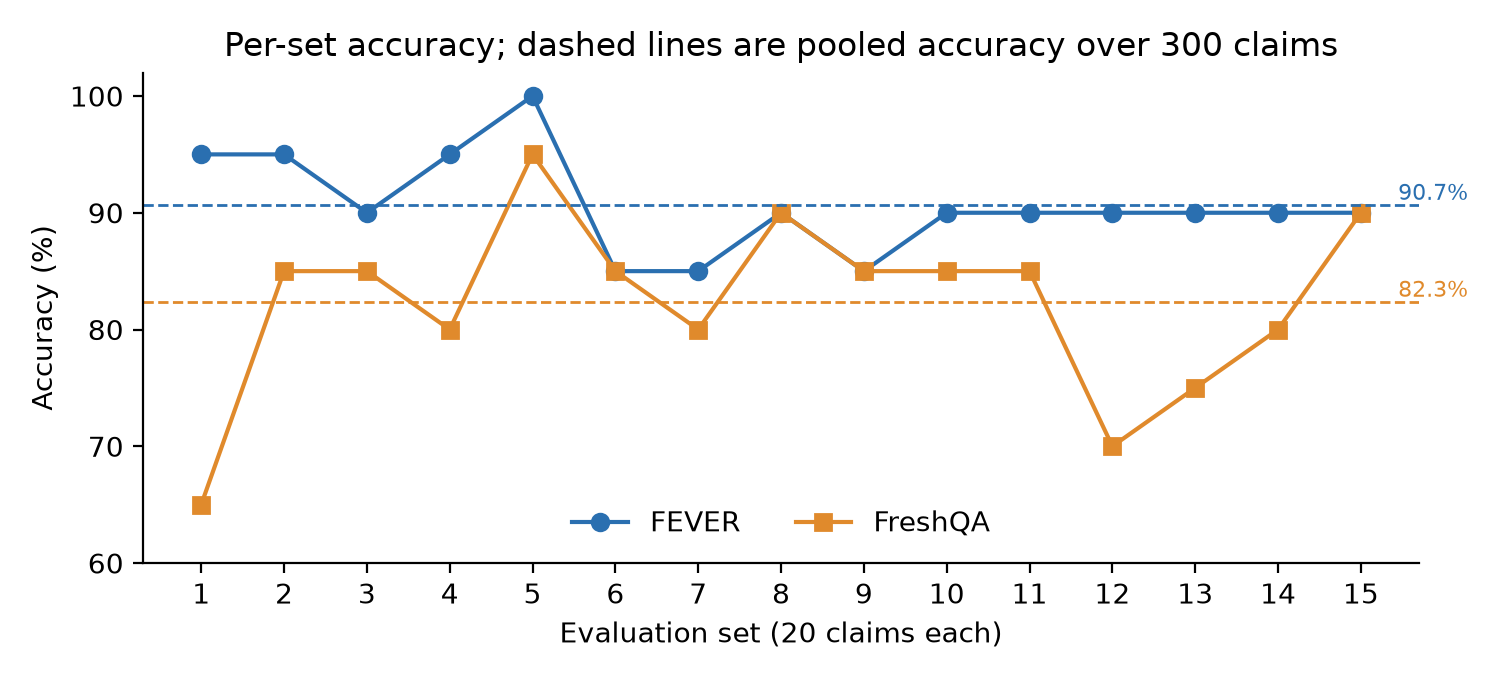
\includegraphics[width=0.95\textwidth]{per_set_accuracy.png}
\caption{Accuracy on each of the fifteen sets of 20 claims. With 20 claims per set, one error moves the accuracy by 5 points; the pooled figures are the ones to quote.}
\label{fig:perset}
\end{figure}

\begin{table}[htbp]
\centering
\caption{Per-set results (correct verdicts out of 20).}
\label{tab:perset}
\small
\begin{tabular}{@{}l*{15}{c}c@{}}
\toprule
Set & 1 & 2 & 3 & 4 & 5 & 6 & 7 & 8 & 9 & 10 & 11 & 12 & 13 & 14 & 15 & Total \\
\midrule
FEVER   & 19 & 19 & 18 & 19 & 20 & 17 & 17 & 18 & 17 & 18 & 18 & 18 & 18 & 18 & 18 & 272 \\
FreshQA & 13 & 17 & 17 & 16 & 19 & 17 & 16 & 18 & 17 & 17 & 17 & 14 & 15 & 16 & 18 & 247 \\
\bottomrule
\end{tabular}
\end{table}

\paragraph{Intervals for precision, recall and $F_1$.} Table~\ref{tab:prf} gives the 95\% intervals of the hallucination-class metrics (Section~\ref{sec:prf-intervals}): Wilson intervals for precision and recall, and percentile-bootstrap intervals for $F_1$ (10{,}000 resamples). Even the lower ends of the precision intervals are above 0.84 (0.885 for FEVER, 0.844 for FreshQA, 0.885 pooled), so false accusations are rare with high confidence; the recall intervals of the two benchmarks barely overlap, which locates the gap between them in missed hallucinations.

\begin{table}[H]
\centering
\caption{Precision, recall and $F_1$ of the hallucination class with 95\% intervals.}
\label{tab:prf}
\begin{tabular}{@{}lccc@{}}
\toprule
Benchmark & Precision (Wilson) & Recall (Wilson) & $F_1$ (bootstrap) \\
\midrule
FEVER & 0.937 [0.885, 0.967] & 0.893 [0.834, 0.933] & 0.915 [0.879, 0.945] \\
FreshQA & 0.907 [0.844, 0.946] & 0.796 [0.724, 0.853] & 0.848 [0.801, 0.890] \\
Pooled & 0.923 [0.885, 0.949] & 0.845 [0.800, 0.882] & 0.882 [0.853, 0.910] \\
\bottomrule
\end{tabular}
\end{table}

\paragraph{Consistency of the runs.} The fifteen sets were evaluated in three runs of five sets each. FEVER scored 95, 87 and 90 of 100 in the three runs: the chi-square test of equal accuracy gives $X^2 = 3.86$ with 2 degrees of freedom, $p = e^{-1.93} = 0.15$. FreshQA scored 82, 85 and 80 ($X^2 = 0.87$, $p = 0.65$). In both cases the runs are consistent with one underlying accuracy.

\paragraph{FEVER versus FreshQA.} FreshQA is significantly harder. The difference in accuracy is 8.3 points (Newcombe 95\% interval [2.9, 13.8] points); the two-proportion $z$-test gives $z = 2.99$, $p = 0.003$, and Fisher's exact test $p = 0.004$. Precision is similar (0.94 against 0.91); the gap lies in recall (0.89 against 0.80) and in abstentions (4 against 15). FreshQA's false premises and claims about the present are more often accepted by the NLI model or left \Unk{} when the evidence does not settle them, and some of its gold answers are contradicted by current evidence (Section~\ref{sec:errors}).

\section{Latency, Routing and Cost}
\label{sec:routing-results}

Table~\ref{tab:latency} gives the latency and the number of LLM calls per claim. Latency was measured end to end, with live Wikipedia, web and Gemini calls, on an Apple M1 laptop. Light LLM calls (query generation and rewriting) took 1.3\,s on average and heavy calls (arbitration, absence evaluation) 2.9\,s.

\begin{table}[H]
\centering
\caption{Latency and LLM usage per claim.}
\label{tab:latency}
\begin{tabular}{@{}lcccc@{}}
\toprule
Benchmark & Mean latency & Median & 90th percentile & LLM calls per claim \\
\midrule
FEVER & 8.5\,s & 8.0\,s & 12.1\,s & 1.05 \\
FreshQA & 11.3\,s & 9.9\,s & 19.5\,s & 1.45 \\
\bottomrule
\end{tabular}
\end{table}

Table~\ref{tab:routes} and Figure~\ref{fig:routing} show how the claims were routed and how accurate each route was. The conformal layer kept 413 of the 600 claims on the fast path, and these were correct 89\% of the time (368 of 413); the 187 claims it passed on, which are the harder ones, were correct 81\% of the time after LLM review (151 of 187).

\begin{table}[H]
\centering
\caption{Claims and accuracy by route.}
\label{tab:routes}
\begin{tabular}{@{}lccc@{}}
\toprule
Benchmark & NLI verdict stands & Lightweight review & Full escalation \\
\midrule
FEVER   & 212 / 229 (93\%) & 30 / 35 (86\%) & 30 / 36 (83\%) \\
FreshQA & 156 / 184 (85\%) & 47 / 54 (87\%) & 44 / 62 (71\%) \\
\bottomrule
\end{tabular}
\end{table}

\begin{figure}[htbp]
\centering
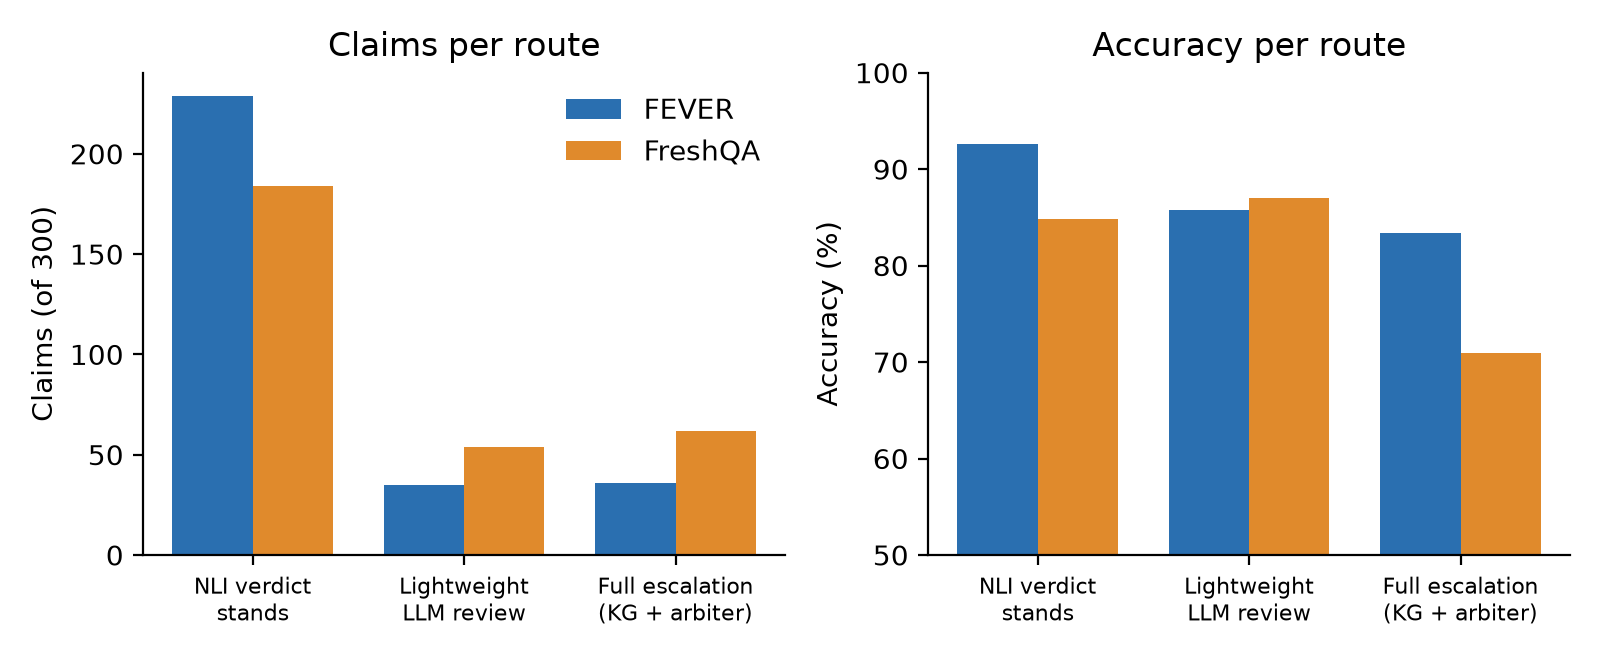
\includegraphics[width=0.95\textwidth]{routing.png}
\caption{Number of claims and accuracy for each route of the cascade.}
\label{fig:routing}
\end{figure}

LLM calls averaged 0.86 per claim when the NLI verdict stood (mostly query generation), 1.88 with a lightweight review and 2.32 with full escalation. Fully escalated claims, which add the Wikidata evidence and arbitration, account for the long tail of the latency distribution.


\section{Effect of the LLM Arbiter}

The computation trace records the NLI verdict just before arbitration, so the arbiter's effect can be measured on every claim it decided (Table~\ref{tab:arbiter}, Figure~\ref{fig:arbiter}).

\begin{table}[htbp]
\centering
\caption{LLM arbiter against the NLI verdict it replaced.}
\label{tab:arbiter}
\begin{tabular}{@{}lccccc@{}}
\toprule
Benchmark & Claims decided & Fixed & Broken & Both right & Both wrong \\
\midrule
FEVER & 71 & 18 & 7 & 42 & 4 \\
FreshQA & 116 & 42 & 8 & 49 & 17 \\
\textbf{Total} & \textbf{187} & \textbf{60} & \textbf{15} & \textbf{91} & \textbf{21} \\
\bottomrule
\end{tabular}
\end{table}

\begin{figure}[htbp]
\centering
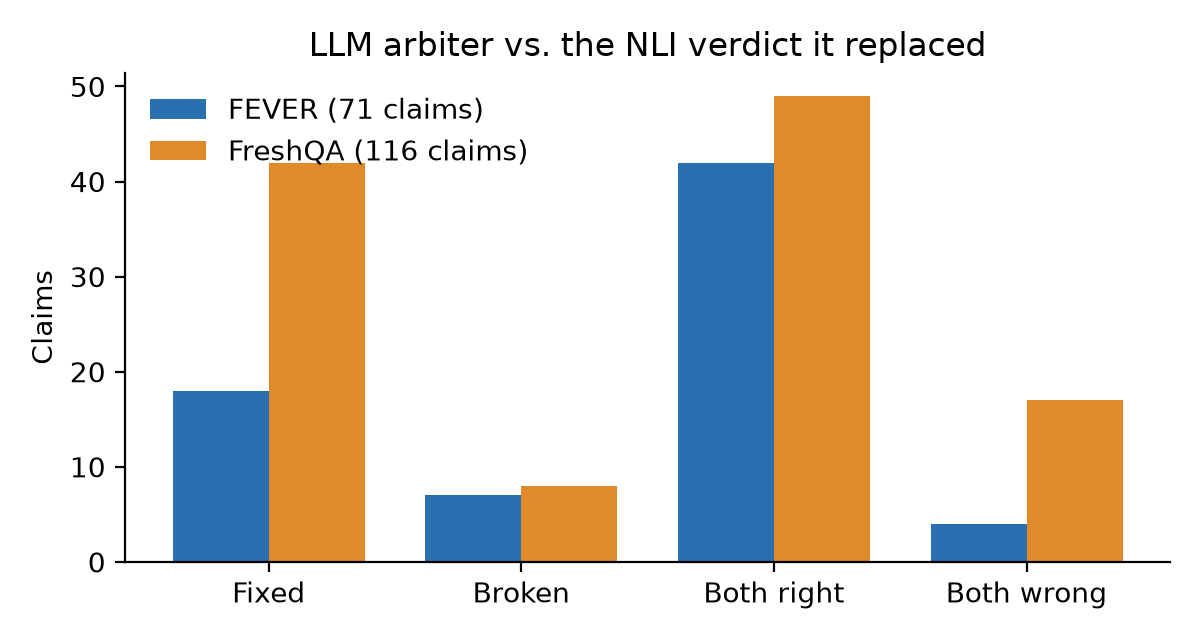
\includegraphics[width=0.72\textwidth]{arbiter_effect.png}
\caption{Claims decided by the LLM arbiter, by whether the NLI verdict and the final verdict were right.}
\label{fig:arbiter}
\end{figure}

The arbiter corrected 60 verdicts and spoiled 15. By the exact McNemar test~\eqref{eq:mcnemar}, $p = 1.6 \times 10^{-7}$: the improvement is highly significant. Per benchmark, FreshQA gives 42 against 8 ($p = 1.2 \times 10^{-6}$) and FEVER 18 against 7 ($p = 0.043$), the latter significant on its own but not after correction for multiple testing (Section~\ref{sec:test-summary}).

\section{Ablation Study}
\label{sec:ablation}

To show what each stage of the cascade contributes, the verdict every claim would have received with that stage removed was reconstructed from its computation trace. The trace records the NLI verdict the scoring rule gave before any LLM review, so removing an LLM stage simply replaces the final verdict of the claims that stage decided by that NLI verdict. The reconstruction is therefore exact and needs no new model run or LLM call. Five variants are compared with the full pipeline:
\begin{itemize}[itemsep=0.2em]
  \item \textbf{Always \Sup}: the trivial detector that never flags a hallucination, as a floor.
  \item \textbf{NLI only, first pass}: the first NLI verdict, with no query rewrite and no LLM verdict. The only LLM calls left are those of query generation for claims outside its fast path.
  \item \textbf{NLI only}: the NLI verdict after the query rewrite, with no LLM verdict.
  \item \textbf{No lightweight review}: lone and contested contradictions are accepted without review (the original ``highest confidence wins'' rule); escalation is kept.
  \item \textbf{No full escalation}: escalated claims keep their NLI verdict (no Wikidata evidence, no arbitration); lightweight reviews are kept.
\end{itemize}
Each variant is compared with the full pipeline by the exact McNemar test on the same claims. The five pooled comparisons form their own family and are Holm-corrected within it; this family is separate from the eight tests of Section~\ref{sec:test-summary}, whose adjusted $p$-values are unchanged.

\begin{table}[H]
\centering
\caption{Ablation study. Accuracy per benchmark and pooled (600 claims), with pooled $F_1$, mean LLM calls per claim, and the exact McNemar test against the full pipeline ($b$: claims right only with the full pipeline; $c$: right only with the variant).}
\label{tab:ablation}
\resizebox{\textwidth}{!}{%
\begin{tabular}{@{}lccccccc@{}}
\toprule
Variant & FEVER & FreshQA & Pooled (Wilson 95\% CI) & Pooled $F_1$ & LLM calls & $b$ / $c$ & $p$ (Holm) \\
\midrule
Always \Sup & 50.0\% & 51.0\% & 50.5\% [46.5, 54.5] & 0.00 & 0.00 & 251 / 35 & $9.7 \times 10^{-41}$ \\
NLI only, first pass & 85.7\% & 62.7\% & 74.2\% [70.5, 77.5] & 0.83 & 0.80 & 88 / 14 & $1.1 \times 10^{-13}$ \\
NLI only & 87.0\% & 71.0\% & 79.0\% [75.6, 82.1] & 0.83 & 0.94 & 60 / 15 & $4.8 \times 10^{-7}$ \\
No lightweight review & 90.3\% & 77.0\% & 83.7\% [80.5, 86.4] & 0.86 & 1.10 & 22 / 5 & $0.0015$ \\
No full escalation & 87.3\% & 76.3\% & 81.8\% [78.5, 84.7] & 0.86 & 1.08 & 38 / 10 & $1.2 \times 10^{-4}$ \\
\textbf{Full pipeline} & \textbf{90.7\%} & \textbf{82.3\%} & \textbf{86.5\% [83.5, 89.0]} & \textbf{0.88} & \textbf{1.25} & -- & -- \\
\bottomrule
\end{tabular}}
\end{table}

\begin{figure}[H]
\centering
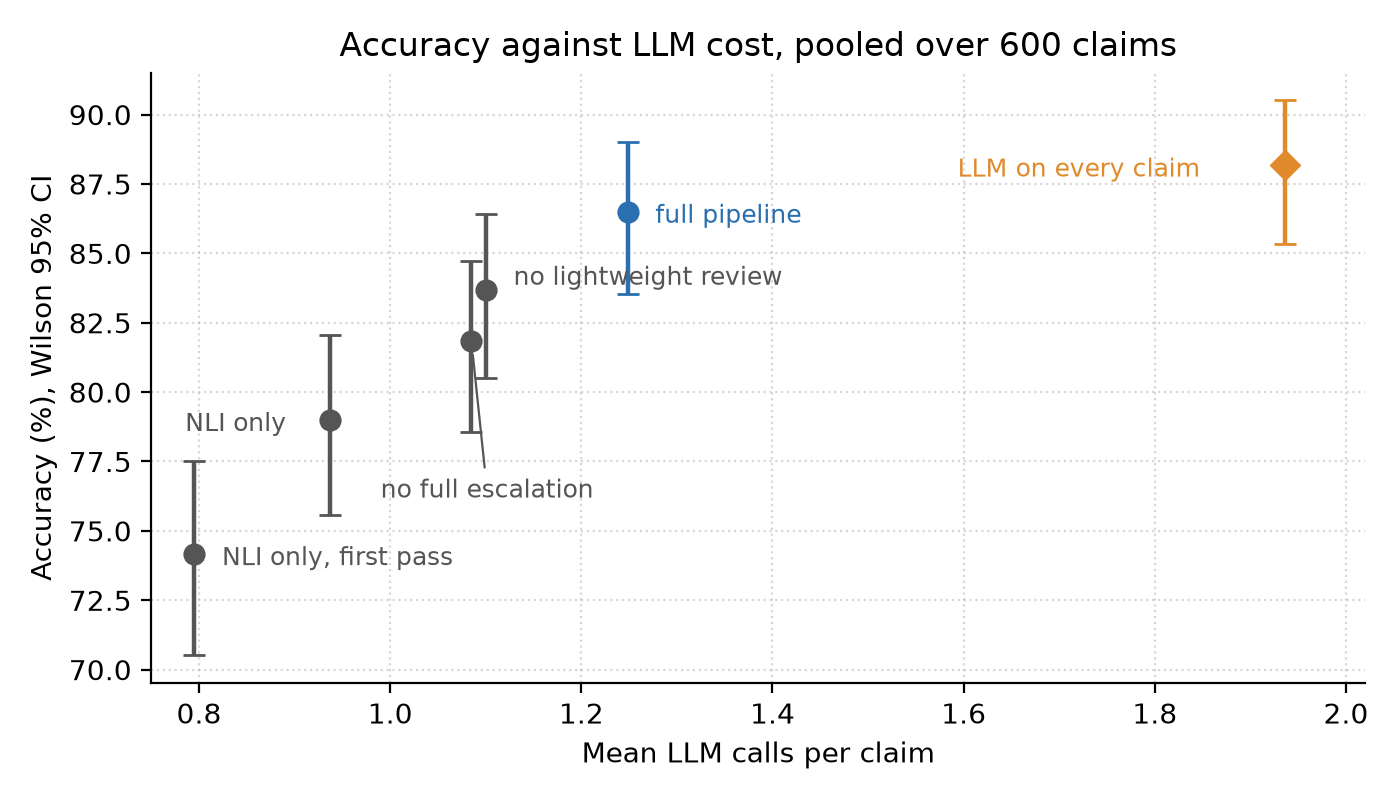
\includegraphics[width=0.8\textwidth]{ablation_cost.png}
\caption{Pooled accuracy of each ablation, and of the LLM-only baseline of Section~\ref{sec:llm-baseline}, against the mean number of LLM calls per claim. ``NLI only'' includes the query rewrite.}
\label{fig:ablation}
\end{figure}

Every stage contributes, and every pooled difference survives the Holm correction (Table~\ref{tab:ablation}, Figure~\ref{fig:ablation}):
\begin{itemize}[itemsep=0.3em]
  \item \textbf{The LLM stages as a whole} raise pooled accuracy from 79.0\% to 86.5\% for 0.31 extra LLM calls per claim, because they are spent only on the claims the conformal layer and the corroboration rule flag.
  \item \textbf{The query rewrite} lifts the NLI verdict from 74.2\% to 79.0\% pooled, almost entirely on FreshQA (62.7\% to 71.0\%), and halves the claims left \Unk{} (85 to 40) for 0.14 extra calls per claim.
  \item \textbf{The lightweight review} matters mostly for \emph{precision}, the property the design protects (Section~\ref{ch:formulation}): without it, precision falls from 0.92 to 0.85 pooled and from 0.91 to 0.79 on FreshQA, because lone and contested NLI contradictions are accepted as false accusations. On FEVER alone the review changes only 7 verdicts (4 against 3) and its effect is not measurable.
  \item \textbf{Full escalation} adds 4.7 points pooled (38 claims fixed, 10 broken) and cuts abstentions from 44 to 19.
\end{itemize}
The two LLM stages are complementary: removing either costs a significant amount of accuracy, and they act on different claims.

\section{Comparison with an LLM-Only Baseline}
\label{sec:llm-baseline}

The ablation removes stages from the cascade. The opposite question is whether the cascade is needed at all: why not let the LLM arbiter decide every claim? To answer it, every claim received one arbitration call on its retrieved evidence, with the same prompt and settings as the live pipeline (dialectical mode, strict premises, the claim's domain). On the 187 claims the LLM already decided in the benchmark run, the two systems are identical by construction, so they can differ only on the 413 claims the NLI verdict settled. Of these, 225 already had an LLM review of the same evidence from the earlier analyses (Sections~\ref{sec:coverage-retrieved} and~\ref{sec:crossfit-results}). The remaining 188 were arbitrated for this comparison (187 calls, since one FEVER claim appears twice), all answered by \code{gemini-3.5-flash-lite}, the model of the benchmark run.

\begin{table}[H]
\centering
\caption{The cascade against an LLM verdict for every claim. The baseline's latency is estimated by adding the mean measured arbitration time (3.0\,s) to every claim the NLI verdict settled.}
\label{tab:llm-baseline}
\resizebox{\textwidth}{!}{%
\begin{tabular}{@{}llcccccc@{}}
\toprule
Benchmark & System & Accuracy (Wilson 95\% CI) & Precision & Recall & $F_1$ & LLM calls per claim & Mean latency \\
\midrule
FEVER & Cascade & 90.7\% [86.8, 93.5] & 0.94 & 0.89 & 0.91 & 1.05 & 8.5\,s \\
 & LLM on every claim & 91.3\% [87.6, 94.0] & 0.94 & 0.91 & 0.93 & 1.81 & 10.8\,s \\
\midrule
FreshQA & Cascade & 82.3\% [77.6, 86.2] & 0.91 & 0.80 & 0.85 & 1.45 & 11.3\,s \\
 & LLM on every claim & 85.0\% [80.5, 88.6] & 0.90 & 0.87 & 0.88 & 2.06 & 13.2\,s \\
\midrule
Pooled & Cascade & 86.5\% [83.5, 89.0] & 0.92 & 0.85 & 0.88 & 1.25 & 9.9\,s \\
 & LLM on every claim & 88.2\% [85.3, 90.5] & 0.92 & 0.89 & 0.91 & 1.94 & 12.0\,s \\
\bottomrule
\end{tabular}}
\end{table}

The paired comparison (Table~\ref{tab:llm-baseline-paired}) uses the exact McNemar test (Section~\ref{sec:tests}). With $b$ claims right only under the cascade and $c$ right only under the baseline, the difference in accuracy and its paired standard error are
\[
  \hat{d} = \frac{c - b}{N}, \qquad \widehat{\mathrm{SE}}(\hat{d}) = \frac{1}{N} \sqrt{b + c - \frac{(c - b)^2}{N}} .
\]
The last column is the number of claims McNemar's test would need for 80\% power against a difference of the observed size (Section~\ref{sec:power}).

\begin{table}[H]
\centering
\caption{Paired comparison of the LLM-only baseline with the cascade.}
\label{tab:llm-baseline-paired}
\resizebox{\textwidth}{!}{%
\begin{tabular}{@{}lccccc@{}}
\toprule
Benchmark & Cascade right only & Baseline right only & $p$ & Difference (95\% CI) & Claims for 80\% power \\
\midrule
FEVER & 7 & 9 & 0.80 & $+0.7$ [$-1.9$, $+3.3$] points & 9{,}417 \\
FreshQA & 11 & 19 & 0.20 & $+2.7$ [$-0.9$, $+6.2$] points & 1{,}102 \\
Pooled & 18 & 28 & 0.18 & $+1.7$ [$-0.5$, $+3.9$] points & 2{,}164 \\
\bottomrule
\end{tabular}}
\end{table}

The result is a trade-off rather than a free gain:
\begin{itemize}[itemsep=0.3em]
  \item \textbf{Accuracy.} Letting the LLM decide every claim is \emph{not} significantly more accurate ($p = 0.18$ pooled). The point estimate favours it by 1.7 points, and the 95\% interval, from $-0.5$ to $+3.9$ points, is compatible both with no difference and with an advantage of a few points. Resolving a difference of this size would need about 2{,}200 claims.
  \item \textbf{Cost.} The cascade makes 0.69 fewer LLM calls per claim (1.25 against 1.94, a saving of 35\%), and is about 2\,s (18\%) faster per claim. The latency estimate slightly favours the baseline, which would also skip the NLI scoring.
  \item \textbf{Where the difference lies.} On the 413 settled claims the NLI verdict is right 368 times and the LLM 378 times. The gain is concentrated on FreshQA (+2.7 points) and in recall (0.80 to 0.87 on FreshQA, precision unchanged): the LLM catches some of the false premises and time-dependent claims that the NLI verdict accepts (Section~\ref{sec:errors}). On FEVER the two are practically identical. The LLM also abstains more often (29 \Unk{} against 19).
\end{itemize}
The cascade therefore buys a 35\% reduction in LLM calls at the price of a possible accuracy loss of at most about 4 points, concentrated in one identifiable class of claims. This points to the targeted escalation of time-dependent and false-premise claims (Chapter~\ref{ch:conclusion}) as the way to close the gap while keeping most of the saving. This comparison is not part of the eight-test family of Section~\ref{sec:test-summary}; being non-significant, it would remain so after any correction.

\paragraph{Caveats.} The LLM verdicts on the settled claims were obtained after the benchmark run, on the same saved evidence and with the same model, but an LLM is not deterministic, so a repeated call can differ on borderline claims. For the 98 escalated claims both systems use the run's verdict, which was reached with the Wikidata evidence; this does not affect the comparison, because those verdicts are identical in both systems.

\section{Validation of the Corroboration Rule by Cross-Fitting}
\label{sec:crossfit-results}

For every claim, its trace determines the verdict it would have received with $m = 1$ (a lone contradiction accepted without review) or $m = 3$ (two agreeing contradictions also reviewed; the 61 additional LLM reviews this requires were all made). On all 600 claims, $m = 1$ gives 503 correct verdicts, $m = 2$ gives 519 and $m = 3$ gives 519. Choosing $m \in \{1, 2, 3\}$ on fourteen of the fifteen sets and scoring the fifteenth (ties going to the smaller $m$, which needs fewer LLM calls) selects $m = 2$ in fourteen of the fifteen folds and in 598 of the 600 leave-one-out folds. The cross-fitted accuracy is 517 of 600, two claims below the 519 of the fixed $m = 2$: the optimism from choosing $m$ on these claims is at most about 0.3 percentage points, far inside the confidence intervals of Table~\ref{tab:main}.

The advantage of $m = 2$ over $m = 1$ rests on 28 claims whose verdict differs: 21 are right only with $m = 2$, 5 only with $m = 1$ and 2 with neither, giving an exact McNemar $p = 0.002$. Against $m = 3$ only 5 verdicts differ (2 against 2, $p = 1$), so the two are indistinguishable, and $m = 3$ would cost 61 more LLM reviews.

\section{Behaviour of the Conformal Layer}

\subsection{Coverage on gold evidence}

The conformal layer was validated on FEVER with gold evidence: $n = 100$ calibration claims and 100 separate test claims (Table~\ref{tab:conformal}, Figure~\ref{fig:conformal}).

\begin{table}[htbp]
\centering
\caption{Conformal coverage on gold evidence (100 test claims, Wilson 95\% intervals).}
\label{tab:conformal}
\begin{tabular}{@{}cccccc@{}}
\toprule
$\alpha$ & Nominal & Empirical coverage & Wilson 95\% CI & Mean set size & $\hat{q}_\alpha$ \\
\midrule
0.05 & 95\% & 99.00\% & [94.55\%, 99.82\%] & 1.63 & 0.9881 \\
\textbf{0.10} & \textbf{90\%} & \textbf{90.00\%} & \textbf{[82.56\%, 94.48\%]} & \textbf{1.26} & \textbf{0.8985} \\
0.15 & 85\% & 85.00\% & [76.72\%, 90.69\%] & 1.13 & 0.7787 \\
0.20 & 80\% & 79.00\% & [70.02\%, 85.83\%] & 1.01 & 0.6286 \\
\bottomrule
\end{tabular}
\end{table}

\begin{figure}[htbp]
\centering
\begin{subfigure}{0.49\textwidth}
  \centering
  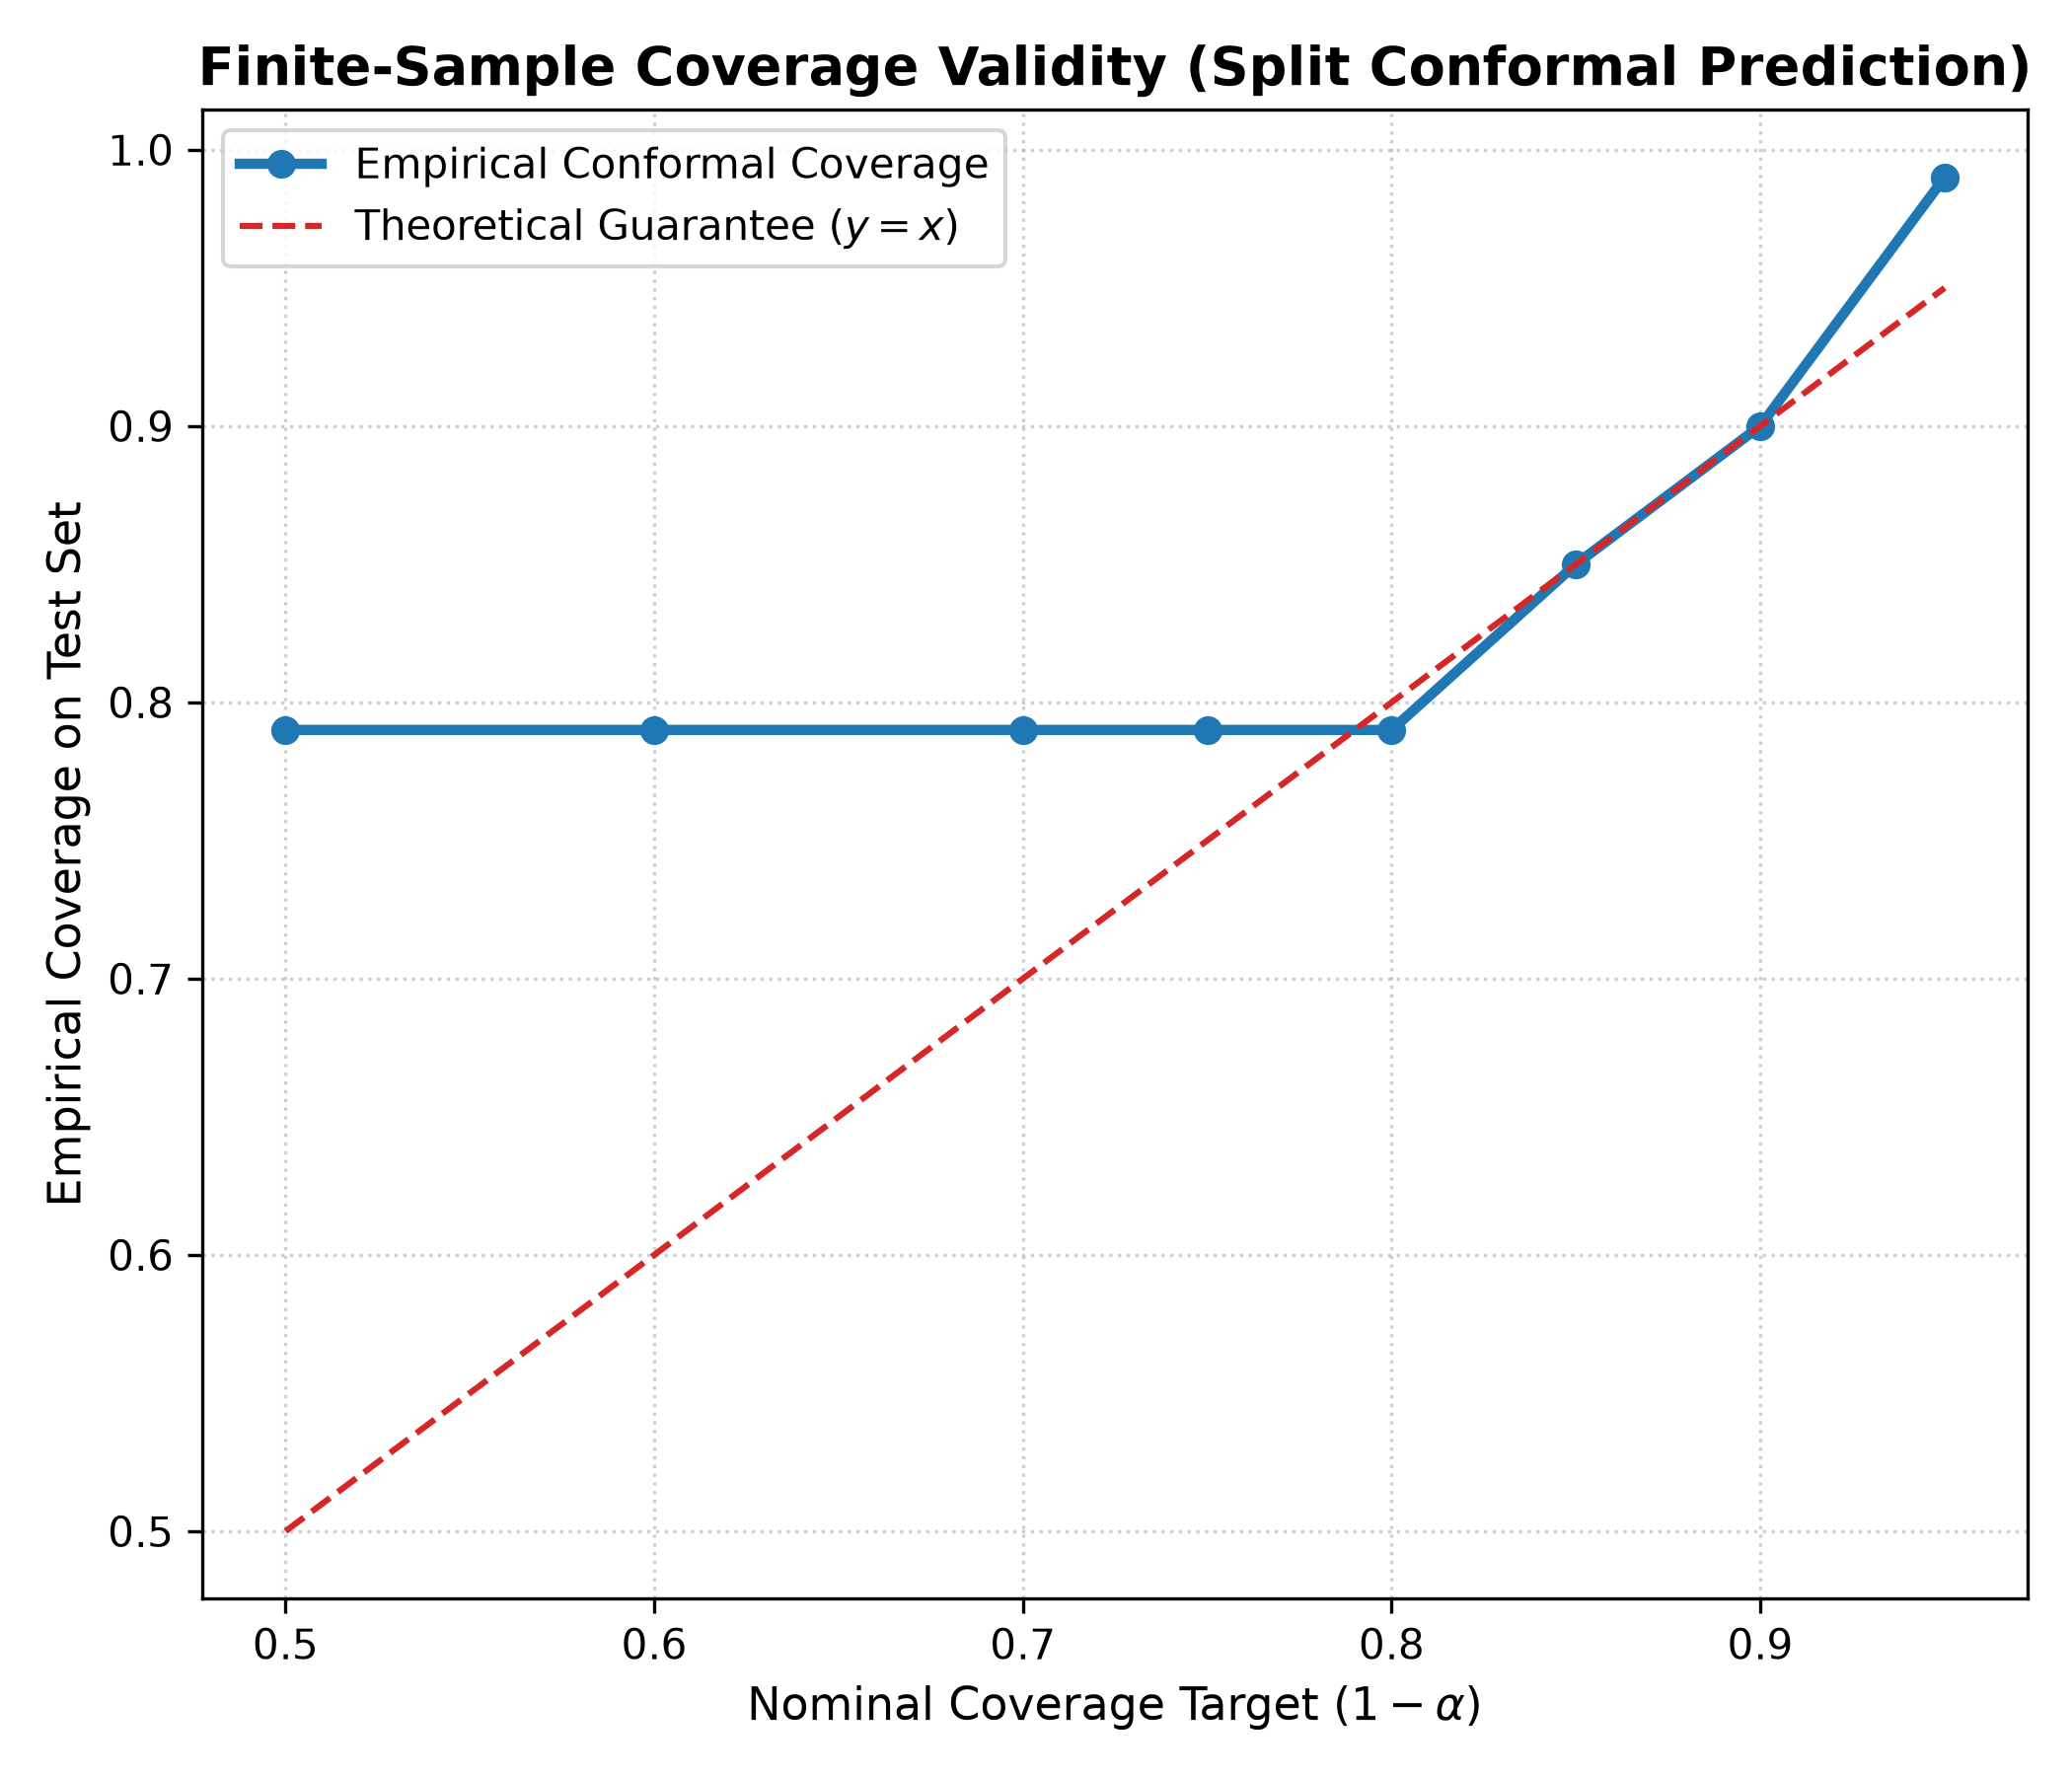
\includegraphics[width=\textwidth]{conformal_coverage_plot.png}
  \caption{Empirical against nominal coverage.}
\end{subfigure}
\hfill
\begin{subfigure}{0.49\textwidth}
  \centering
  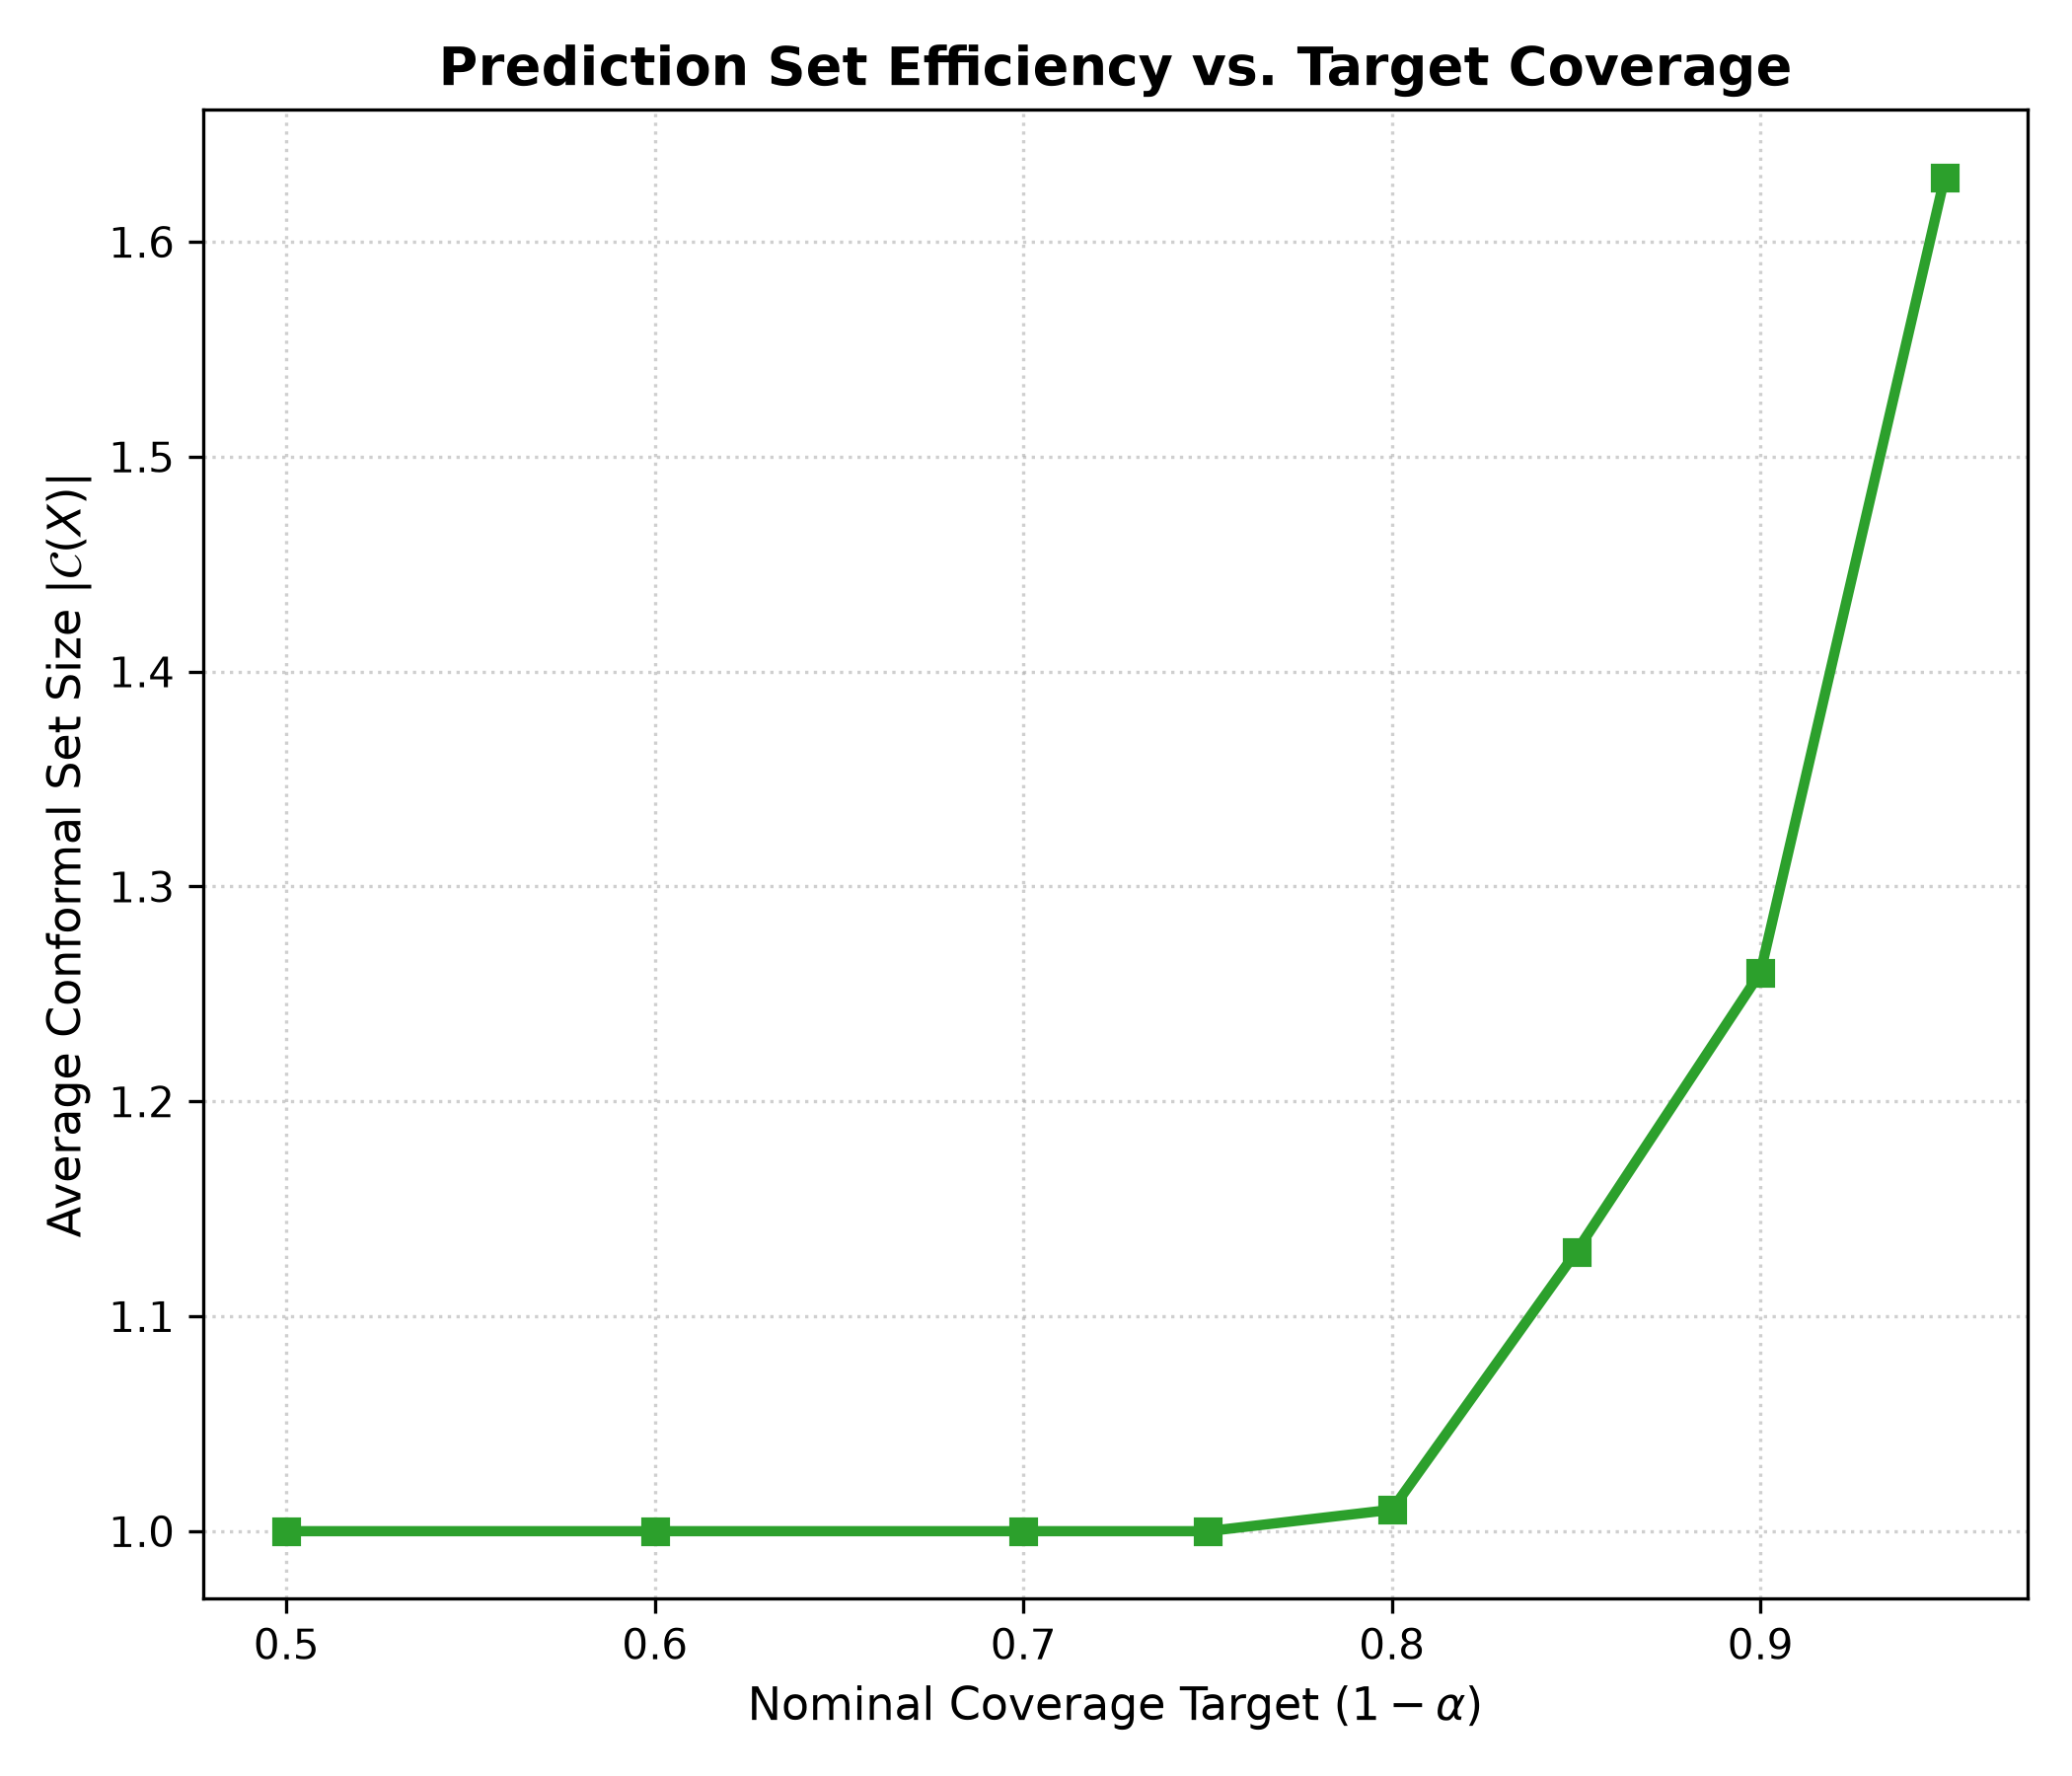
\includegraphics[width=\textwidth]{conformal_set_size_plot.png}
  \caption{Mean prediction-set size.}
\end{subfigure}
\caption{Split conformal prediction on FEVER with gold evidence.}
\label{fig:conformal}
\end{figure}

At the production level $\alpha = 0.10$ the empirical coverage equals the nominal 90\% with only 1.26 labels per set on average, so most claims receive a decisive singleton. For $\alpha \ge 0.20$ the sets are almost always singletons, so coverage cannot fall further and stays at the raw accuracy of the NLI model on gold evidence (79\%).

\subsection{Coverage on retrieved evidence}
\label{sec:coverage-retrieved}

In deployment the NLI probabilities are computed on \emph{retrieved} snippets, which are noisier than FEVER's gold evidence, so the exchangeability assumption of Theorem~\ref{thm:coverage} does not hold. Measuring coverage on the 600 evaluation claims (Table~\ref{tab:coverage-retrieved}, Figure~\ref{fig:coverage-retrieved}) confirms the consequence. To recalibrate without bias, the claims were split into two halves, and each half was tested with the $\hat{q}$ calibrated on the other.

\begin{table}[htbp]
\centering
\caption{Conformal coverage on retrieved evidence (600 claims).}
\label{tab:coverage-retrieved}
\small
\begin{tabularx}{\textwidth}{@{}Xcccc@{}}
\toprule
Threshold & Coverage & Wilson 95\% CI & Mean set size & Accuracy (FEVER / FreshQA) \\
\midrule
Current, $\hat{q} = 0.8985$ (gold-evidence calibration) & 83.2\% & [80.0\%, 85.9\%] & 1.18 & 90.7\% / 82.3\% (measured) \\
Recalibrated on retrieved evidence, $\hat{q} \approx 0.990$--$0.995$ & 90.3\% & [87.7\%, 92.4\%] & 1.80 & 92.3\% / 84.3\% (estimated) \\
\bottomrule
\end{tabularx}
\end{table}

\begin{figure}[htbp]
\centering
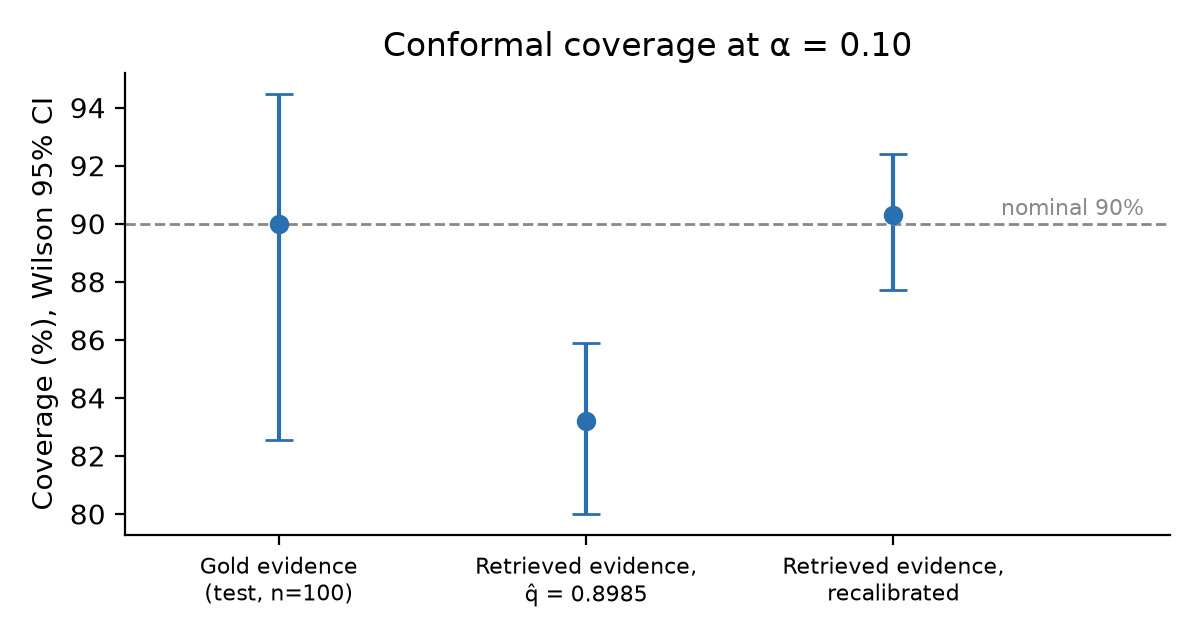
\includegraphics[width=0.7\textwidth]{coverage_retrieved.png}
\caption{Conformal coverage at $\alpha = 0.10$ on gold and retrieved evidence, with Wilson 95\% intervals.}
\label{fig:coverage-retrieved}
\end{figure}

With the current threshold, coverage on live evidence is measurably below the nominal 90\%: the whole interval lies below it, as the exchangeability argument predicts. Recalibrating restores 90.3\% coverage, but only with a threshold that admits any label above about 0.5--1\% probability, so 181 more claims would be escalated. The estimated pooled accuracy would rise from 86.5\% to 88.3\% (530 against 519 correct), but the gain is not significant: the recalibrated verdicts fix 21 claims and break 10 (exact McNemar $p = 0.07$), at the cost of an LLM review for almost a third of all claims. The production threshold is therefore kept, and the conformal set is described as what it is in deployment: a calibrated escalation trigger with 83.2\% measured coverage, not a 90\% guarantee.

\subsection{Class-conditional coverage and alternative scores}
\label{sec:conformal-variants}

Two questions remain: whether the shortfall falls equally on false and true claims, and whether a different conformal procedure (Section~\ref{sec:scores}) would do better. Four procedures were compared at $\alpha = 0.10$: the production layer (LAC), Mondrian LAC, non-randomised APS, and randomised APS as a reference (one uniform draw per claim, fixed seed). Each was calibrated on the 100 production calibration claims and evaluated in three settings: on the other 100 gold-evidence claims; on the 600 benchmark claims with the gold-evidence quantiles, as deployed; and on the 600 claims recalibrated by the same two-fold cross-fitting as in Table~\ref{tab:coverage-retrieved}. For the benchmark claims, the routing rule~\eqref{eq:escalate} was applied to each procedure's sets. A claim keeps its verdict unless its route changes. A claim that no longer goes to the LLM takes its NLI verdict, and a newly escalated claim takes the LLM verdict on its saved evidence from Section~\ref{sec:llm-baseline}, so no new LLM call is needed. As a check, the production layer reproduces the routing of the run exactly (98 escalations, no verdict changed).

\begin{table}[H]
\centering
\caption{Conformal procedures on gold evidence (calibrated on 100 claims, tested on 100: 45 false, 55 true).}
\label{tab:conformal-gold}
\small
\begin{tabular}{@{}lcccc@{}}
\toprule
Procedure & Coverage (95\% CI) & False claims & True claims & Mean set size \\
\midrule
LAC (production) & 90.0\% [82.6, 94.5] & 95.6\% & 85.5\% & 1.26 \\
Mondrian LAC & 92.0\% [85.0, 95.9] & 84.4\% & 98.2\% & 1.26 \\
APS & 95.0\% [88.8, 97.8] & 95.6\% & 94.5\% & 1.76 \\
Randomised APS & 92.0\% [85.0, 95.9] & 95.6\% & 89.1\% & 1.41 \\
\bottomrule
\end{tabular}
\end{table}

\begin{table}[H]
\centering
\caption{Conformal procedures on retrieved evidence (600 claims: 297 false, 303 true), with the number of claims escalated, the estimated pooled accuracy, and the exact McNemar test against the pipeline as run ($b$: right only as run; $c$: right only with the procedure).}
\label{tab:conformal-variants}
\resizebox{\textwidth}{!}{%
\begin{tabular}{@{}llcccccccc@{}}
\toprule
Quantiles & Procedure & Coverage (Wilson 95\% CI) & False claims & True claims & Set size & Escalated & Accuracy & $b$ / $c$ & $p$ \\
\midrule
Gold-evidence & LAC (production) & 83.2\% [80.0, 85.9] & 84.5\% & 81.8\% & 1.18 & 98 & 86.5\% & -- & -- \\
(as deployed) & Mondrian LAC & 83.3\% [80.1, 86.1] & 79.8\% & 86.8\% & 1.19 & 125 & 87.2\% & 1 / 5 & 0.22 \\
 & APS & 86.7\% [83.7, 89.2] & 87.5\% & 85.8\% & 1.83 & 483 & 88.8\% & 14 / 28 & 0.044 \\
 & Randomised APS & 85.0\% [81.9, 87.6] & 86.2\% & 83.8\% & 1.35 & 184 & 86.8\% & 7 / 9 & 0.80 \\
\midrule
Recalibrated & LAC & 90.3\% [87.7, 92.4] & 92.6\% & 88.1\% & 1.80 & 339 & 88.3\% & 10 / 21 & 0.071 \\
(cross-fitted) & Mondrian LAC & 90.3\% [87.7, 92.4] & 89.6\% & 91.1\% & 1.82 & 350 & 88.0\% & 12 / 21 & 0.16 \\
 & APS & 90.2\% [87.5, 92.3] & 89.9\% & 90.4\% & 2.33 & 600 & 88.2\% & 18 / 28 & 0.18 \\
 & Randomised APS & 90.2\% [87.5, 92.3] & 92.3\% & 88.1\% & 1.90 & 388 & 88.0\% & 15 / 24 & 0.20 \\
\bottomrule
\end{tabular}}
\end{table}

\begin{figure}[H]
\centering
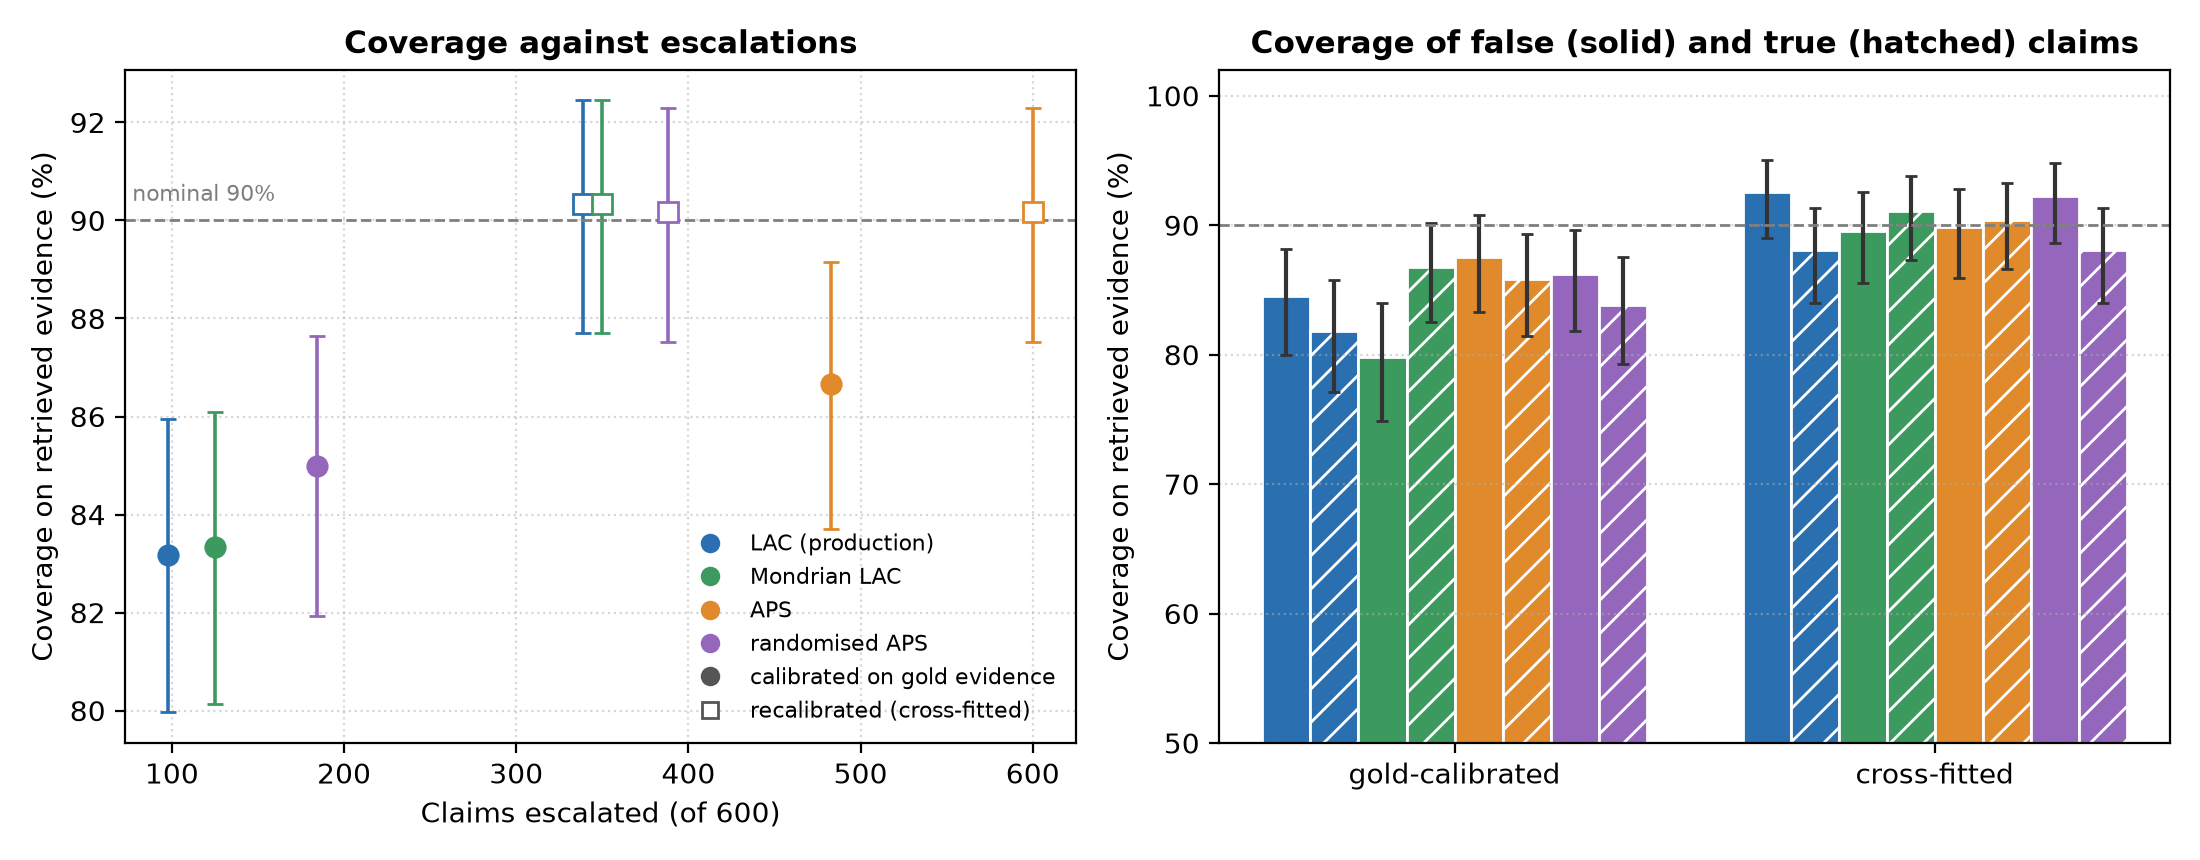
\includegraphics[width=\textwidth]{conformal_variants.png}
\caption{Conformal procedures on retrieved evidence. Left: coverage against the number of claims escalated, with gold-evidence quantiles (filled) and cross-fitted recalibration (open). Right: coverage of false (solid) and true (hatched) claims, with Wilson 95\% intervals.}
\label{fig:conformal-variants}
\end{figure}

The results (Tables~\ref{tab:conformal-gold} and~\ref{tab:conformal-variants}, Figure~\ref{fig:conformal-variants}) answer both questions:
\begin{itemize}[itemsep=0.3em]
  \item \textbf{The shortfall is shared by both classes.} On retrieved evidence the production layer covers 84.5\% of false claims and 81.8\% of true claims, and the two intervals overlap. Hallucinations are not disproportionately missed. On gold evidence the imbalance runs the other way (95.6\% against 85.5\%), because false FEVER claims are refuted confidently by their gold evidence.
  \item \textbf{Mondrian balances the classes, as Theorem~\ref{thm:mondrian} predicts, but does not repair the shift.} Recalibrated, it brings both classes close to 90\% (89.6\% and 91.1\%, against 92.6\% and 88.1\% for LAC) at almost the same cost (350 escalations against 339). With the gold-evidence quantiles its overall coverage stays at 83.3\%. On gold evidence its false-claim coverage of 84.4\% is below 90\%, but with 45 test claims and about 50 calibration claims per class this lies within the expected variation of one calibration.
  \item \textbf{Non-randomised APS degenerates as Remark~\ref{rem:aps} predicts.} Its quantile is 0.9998 on gold evidence and 1.0000 when recalibrated, so it escalates 483 and 600 claims. Its higher coverage and accuracy come only from sending almost every claim to the LLM; recalibrated, it reproduces the LLM-only baseline of Section~\ref{sec:llm-baseline} exactly.
  \item \textbf{Randomised APS is less efficient than LAC.} It reaches 90\% coverage only with 388 escalations, against 339 for LAC, with no gain in accuracy.
\end{itemize}

None of the accuracy differences in Table~\ref{tab:conformal-variants} survives a Holm correction over its seven comparisons; the smallest $p$, 0.044, becomes 0.31. LAC is the most efficient of the four procedures, and no choice of score closes the gap between 83\% and 90\% without escalating hundreds more claims. The shortfall comes from the difference between gold and retrieved evidence, not from the procedure, which is why the production layer is kept and reported as a calibrated escalation trigger.

\section{Calibration of the NLI Probabilities}

Calibration was evaluated on the 560 benchmark claims whose final NLI verdict is \Sup{} or \Con. The temperature $T$ was cross-fitted: each set was scored with the $T$ fitted on the other sets (the fitted values range from 2.43 to 2.56; on all claims $T = 2.48$). A paired bootstrap with 10{,}000 resamples~\citep{efron1993bootstrap} gives 95\% intervals for each change (Table~\ref{tab:calibration}).

\begin{table}[htbp]
\centering
\caption{Calibration before and after temperature scaling (560 claims).}
\label{tab:calibration}
\begin{tabular}{@{}lccc@{}}
\toprule
Metric & Raw & Temperature-scaled & Change (95\% bootstrap interval) \\
\midrule
NLL & 0.898 & 0.585 & $-0.313$ [$-0.423$, $-0.207$] \\
Brier score & 0.296 & 0.286 & $-0.010$ [$-0.028$, $+0.006$] \\
ECE & 11.4\% & 5.7\% & $-5.7$ points [$-8.9$, $-0.4$] \\
Mean confidence & 95.7\% & 79.6\% & -- \\
Accuracy & 84.6\% & 84.6\% & unchanged \\
\bottomrule
\end{tabular}
\end{table}

\begin{figure}[htbp]
\centering
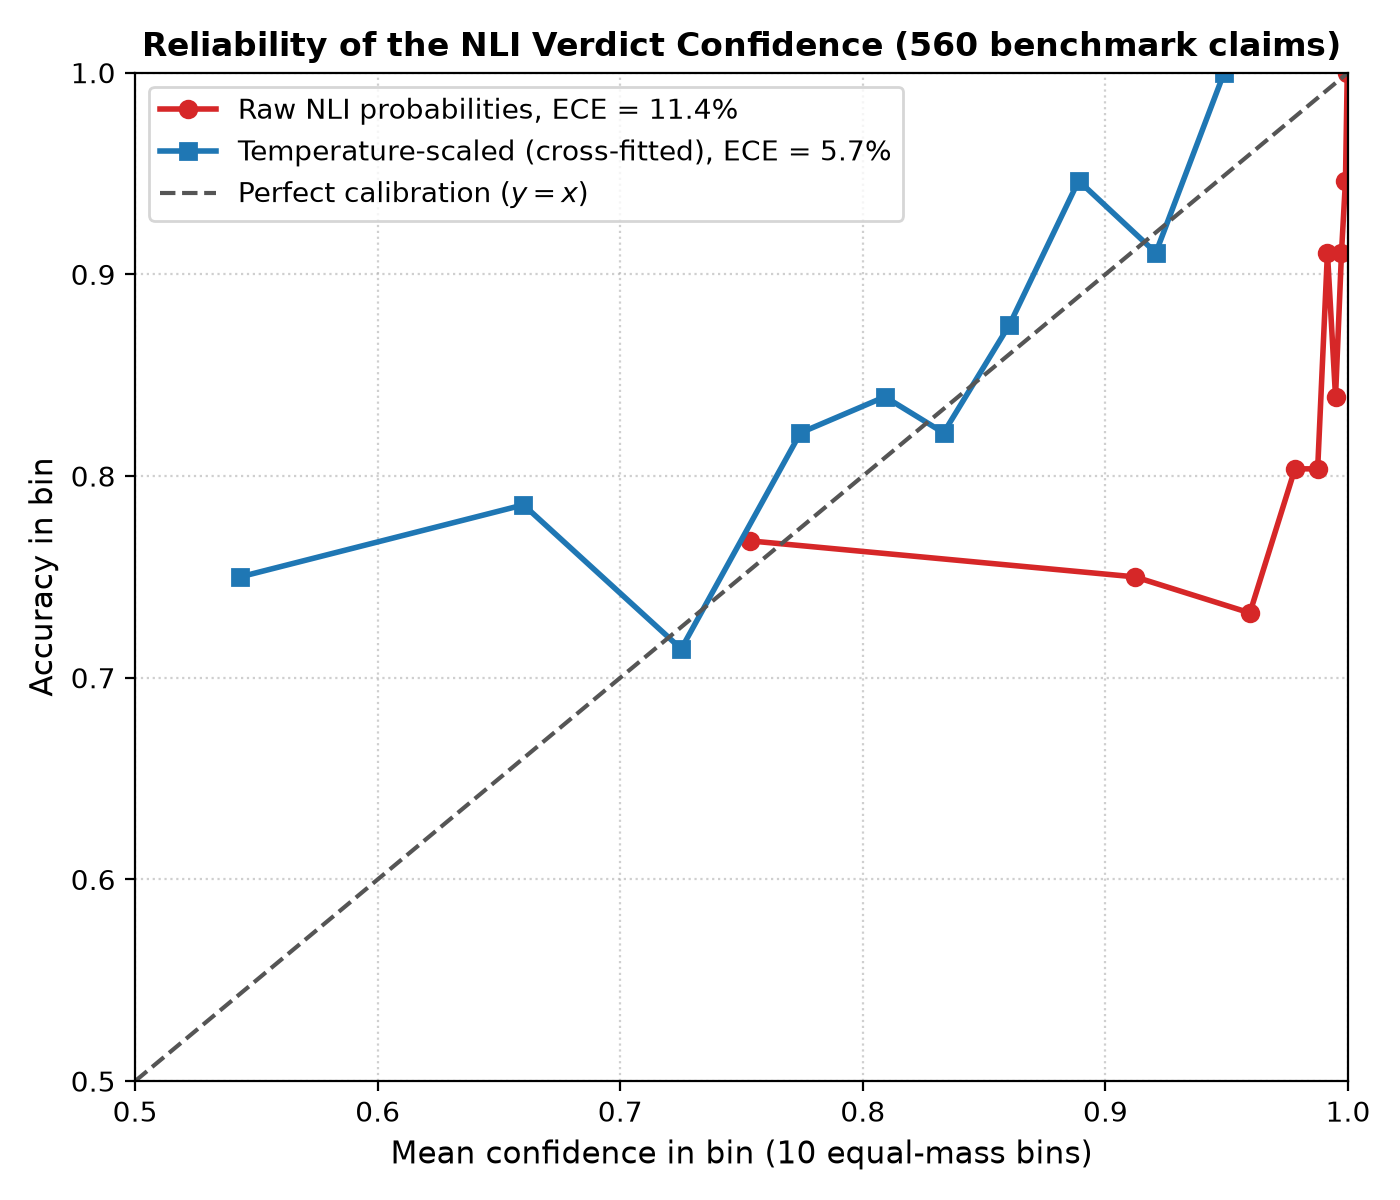
\includegraphics[width=0.75\textwidth]{calibration_reliability.png}
\caption{Reliability diagram of the NLI confidence before and after temperature scaling (ten bins of 56 claims).}
\label{fig:reliability}
\end{figure}

The raw confidences crowd above 0.95 while accuracy ranges from 73\% to 100\% across bins. After scaling, the stated confidence tracks accuracy in most bins (Figure~\ref{fig:reliability}). The NLL improvement is clearly significant, because it comes from the confident mistakes that scaling softens, and so is the halving of the ECE. The Brier improvement is not: the Brier score also rewards ranking right verdicts above wrong ones, which a single temperature hardly changes. Indeed the raw confidence separates right from wrong verdicts with an AUROC of 0.672 and the scaled confidence with 0.673. For the \emph{Bones} example, the logits $(4.084, -0.974, -3.995)$ become $(1.646, -0.393, -1.610)$, and the confidence in \Con{} falls from 0.993 to 0.856. Decisions keep the raw scale, because the thresholds and the conformal quantile were set and measured on it; the calibrated confidence is reported alongside.

A two-parameter Platt scaling, cross-fitted in the same way, reaches a top-label ECE of 5.5\% against 5.7\%, a difference within noise; temperature scaling is kept because it has one parameter and yields a full probability vector.

\section{Selective Prediction}
\label{sec:selective-results}

The pipeline already abstains on 4 FEVER and 15 FreshQA claims. Section~\ref{sec:selective} asks a further question: if the detector were allowed to abstain on more claims, would its NLI confidence choose the right ones? The answered claims were ranked by the NLI probability of their final verdict, and the detector abstained on the least confident first (Figure~\ref{fig:risk-coverage}, Table~\ref{tab:selective}). The AURC interval is a percentile bootstrap over the answered claims (1{,}000 resamples).

\begin{figure}[H]
\centering
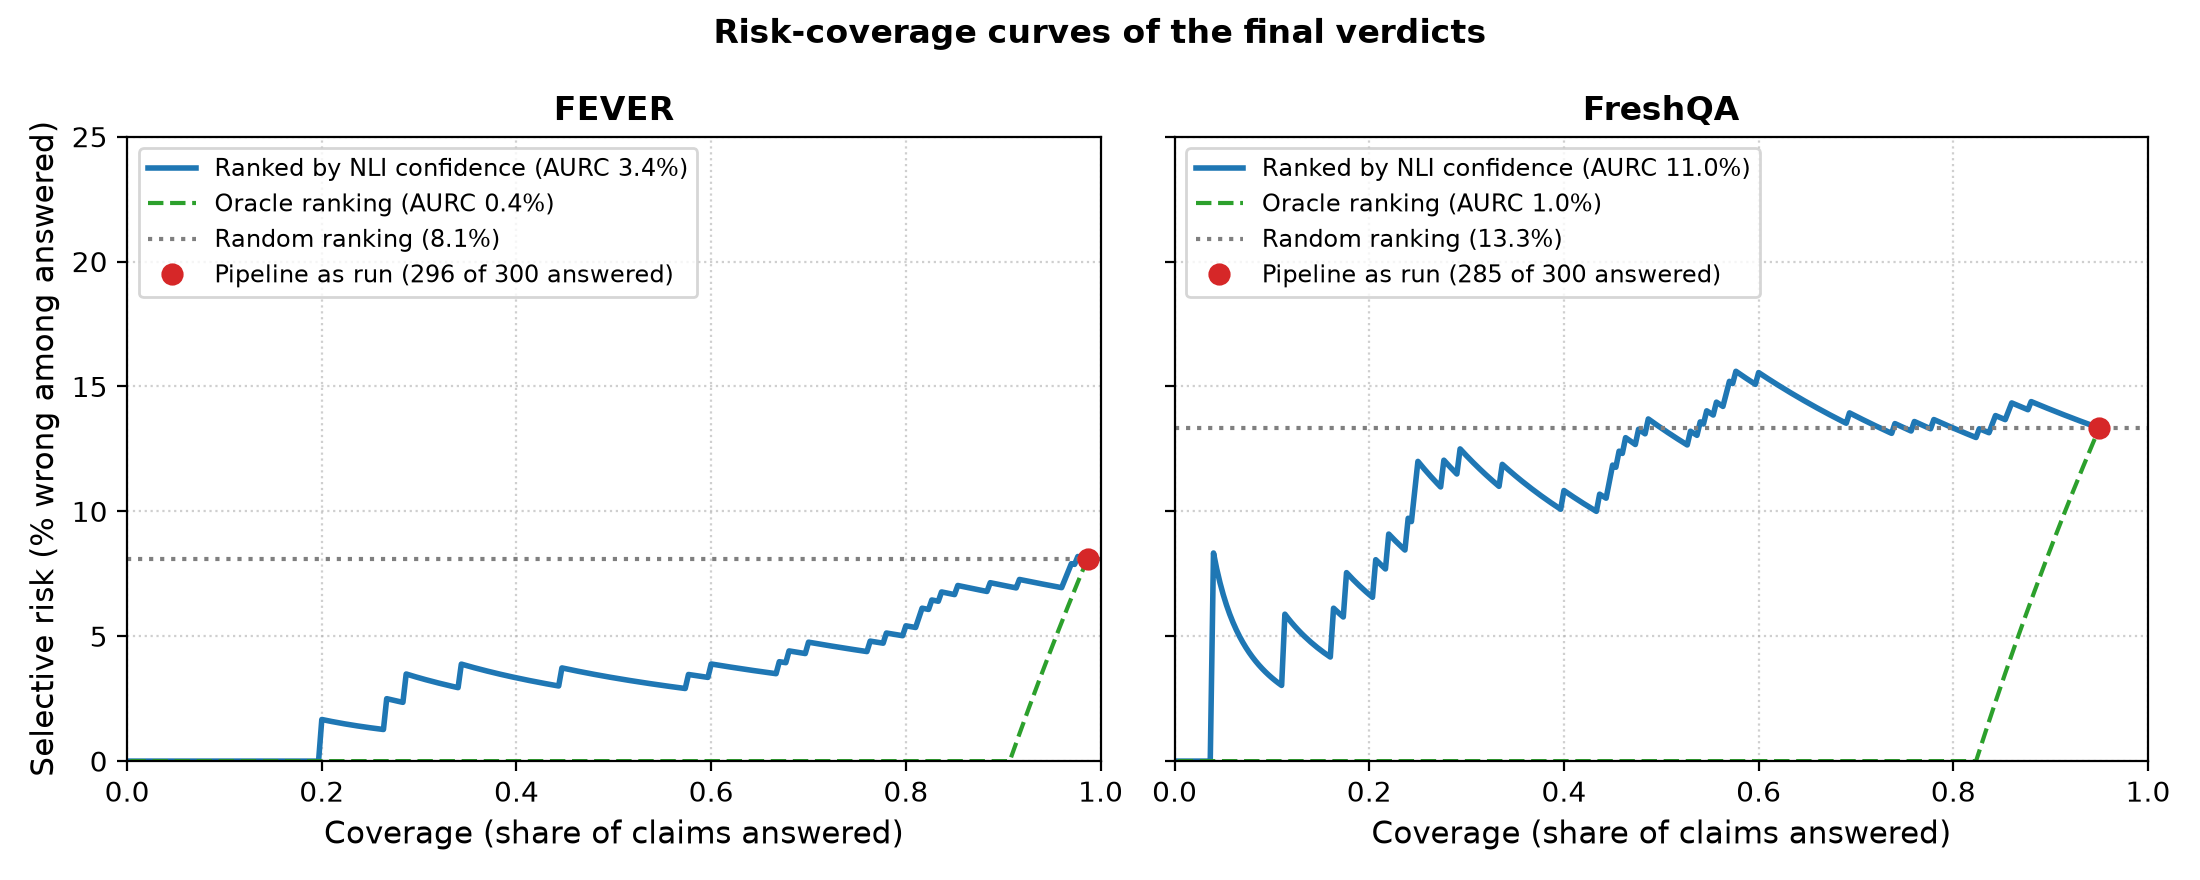
\includegraphics[width=\textwidth]{risk_coverage.png}
\caption{Risk--coverage curves of the final verdicts, ranked by the NLI probability of the verdict, against the oracle and random rankings of Proposition~\ref{prop:aurc}. The red point is the pipeline as run.}
\label{fig:risk-coverage}
\end{figure}

\begin{table}[H]
\centering
\caption{Selective prediction. Selective risk is the error rate among answered claims.}
\label{tab:selective}
\resizebox{\textwidth}{!}{%
\begin{tabular}{@{}lcccccc@{}}
\toprule
Benchmark & Answered & Risk as run & AURC (95\% CI) & Oracle & Random & Risk at 80\% / 90\% coverage \\
\midrule
FEVER & 296 / 300 & 8.1\% & 3.4\% [1.5, 5.5] & 0.35\% & 8.1\% & 5.4\% / 7.0\% \\
FreshQA & 285 / 300 & 13.3\% & 11.0\% [6.8, 16.1] & 0.95\% & 13.3\% & 13.3\% / 14.1\% \\
\bottomrule
\end{tabular}}
\end{table}

On FEVER the confidence is informative. Its AURC is less than half the random value, and abstaining on the least confident fifth of the claims lowers the error rate among the rest from 8.1\% to 5.4\%. On FreshQA the confidence helps only among the most confident quarter of the claims; at 80\% and 90\% coverage the selective risk equals the overall error rate, so abstaining by confidence would not help. The reason lies in FreshQA's errors (Section~\ref{sec:errors}): most are confident NLI fast-path errors on time-dependent claims and false premises, or claims whose gold label is out of date, and the NLI confidence cannot identify either kind. Both curves stay far above the oracle. This agrees with the moderate AUROC of the confidence (0.67, Section~\ref{sec:calibration}) and confirms that better abstention and routing need signals beyond the NLI confidence.

\section{Summary of Hypothesis Tests}
\label{sec:test-summary}

Table~\ref{tab:tests} collects the eight hypothesis tests reported, with their Holm and Benjamini--Hochberg adjusted $p$-values (Section~\ref{sec:multiple}).

\begin{table}[htbp]
\centering
\caption{All hypothesis tests with multiple-comparison corrections. Bold marks an adjusted $p < 0.05$.}
\label{tab:tests}
\small
\begin{tabularx}{\textwidth}{@{}Xllll@{}}
\toprule
Comparison & Test & $p$ & Holm & BH \\
\midrule
LLM arbiter vs NLI verdict, both benchmarks (60 fixed, 15 broken) & exact McNemar & $1.6 \times 10^{-7}$ & $\mathbf{1.3 \times 10^{-6}}$ & $\mathbf{1.3 \times 10^{-6}}$ \\
LLM arbiter, FreshQA (42 fixed, 8 broken) & exact McNemar & $1.2 \times 10^{-6}$ & $\mathbf{8.1 \times 10^{-6}}$ & $\mathbf{4.7 \times 10^{-6}}$ \\
Corroboration rule, $m = 2$ vs $m = 1$ (21 vs 5) & exact McNemar & 0.002 & \textbf{0.015} & \textbf{0.006} \\
FEVER vs FreshQA accuracy (90.7\% vs 82.3\%) & two-proportion $z$ & 0.003 & \textbf{0.015} & \textbf{0.006} \\
LLM arbiter, FEVER (18 fixed, 7 broken) & exact McNemar & 0.043 & 0.17 & 0.069 \\
FEVER, the three runs (95, 87, 90 of 100) & $\chi^2_2$ & 0.15 & 0.44 & 0.19 \\
FreshQA, the three runs (82, 85, 80 of 100) & $\chi^2_2$ & 0.65 & 1 & 0.74 \\
Corroboration rule, $m = 2$ vs $m = 3$ (2 vs 2) & exact McNemar & 1 & 1 & 1 \\
\bottomrule
\end{tabularx}
\end{table}

The ablation comparisons of Section~\ref{sec:ablation} form a separate family with their own Holm correction and are not included here. Four findings survive both corrections: the arbiter improves on the NLI verdict (pooled, and on FreshQA alone), $m = 2$ beats $m = 1$, and FreshQA is harder than FEVER. The arbiter's effect on FEVER alone is significant only before correction; the runs of each benchmark are mutually consistent; and $m = 2$ and $m = 3$ cannot be told apart.

\paragraph{Power.} Non-significant results must be read against the power of the test. With 300 claims per benchmark, a true difference of 5 points between benchmarks (around 86.5\% accuracy) would be detected with only 43\% power (44\% in simulation), 7.5 points with 77\% and 10 points with 95\%; 80\% power for a 5-point difference would need 733 claims per benchmark. At the observed difference of 8.3 points, 263 claims per benchmark give 80\% power, so the present 300 suffice. For the arbiter on FEVER ($\psi = 0.35$, $\delta = 0.15$) about 113 arbitrated claims, roughly 480 FEVER claims, would be needed, against 71 now. The non-significant FEVER arbiter result is therefore expected at this sample size and does not show that the arbiter has no effect there.

\section{Error Analysis}
\label{sec:errors}

\subsection{FEVER}

The 28 FEVER errors are 9 false accusations, 15 missed hallucinations and 4 abstentions. By the stage that produced them:
\begin{itemize}[itemsep=0.3em]
  \item \textbf{NLI fast-path errors (17).} Settled without LLM review. True claims were contradicted by several agreeing snippets that describe a related but different fact (e.g.\ \emph{``Taran Killam is an American writer''}, contradicted by snippets describing him as an actor and comedian), or because the query retrieved the wrong sense of an ambiguous name (\emph{``Tool is a band''} retrieved the article on tools as implements). False claims were supported by a decisive snippet about a closely related fact (\emph{``Saturn is the second-largest moon in the Solar System''}, supported by a sentence stating this of Titan, Saturn's largest moon), or differing from the evidence in a single number, title or role.
  \item \textbf{Arbiter errors (7).} Mostly over-generous inference, such as accepting \emph{``Heavy metal music was developed in Europe''} from evidence that it developed ``largely in the United Kingdom and United States'', or reading a present-tense claim as contradicted by evidence of a past state.
  \item \textbf{Abstentions (4).} The evidence covered the topic but not the specific fact, and the arbiter, finding no statement either way, abstained.
\end{itemize}

\subsection{FreshQA}

\begin{table}[htbp]
\centering
\caption{FreshQA accuracy by fact type.}
\label{tab:facttype}
\begin{tabular}{@{}lcccc@{}}
\toprule
Fact type & Claims & Correct & Wrong & Accuracy \\
\midrule
never-changing & 155 & 130 & 25 & 83.9\% \\
slow-changing & 145 & 117 & 28 & 80.7\% \\
\bottomrule
\end{tabular}
\end{table}

The 53 FreshQA errors fall into four groups:
\begin{itemize}[itemsep=0.3em]
  \item \textbf{NLI fast-path errors (24).} Negations, claims about the present matched to past evidence (the NLI model ignores words such as \emph{``currently''}), false premises accepted from related evidence (\emph{``Hikaru Nakamura became the World Chess Champion''}, supported by snippets on his Fischer Random world title), and web pages that themselves assert a false claim.
  \item \textbf{Abstentions (15).} In all but one, the evidence covered the topic but not the specific number, date or ranking the claim asserts. In one case the claim-echo filter removed the only snippets stating the fact, because a genuine paraphrase of a short claim reached the 80\% overlap threshold.
  \item \textbf{Gold labels contradicted by current evidence (11).} The evidence retrieved in 2026 states a different value from the dated gold answer (for example, a later record time or a changed station count). In these cases the detector followed the evidence; even slow-changing labels drift out of date.
  \item \textbf{Arbiter errors (3).} Including one case in which the arbiter counted an item from a different, similarly named list.
\end{itemize}

Across both benchmarks, 41 of the 81 errors are NLI fast-path errors and 19 are abstentions, which identifies the two main levers for improvement: routing the claim types on which NLI is systematically weak (negations, time-dependent claims) to the arbiter, and better retrieval of specific numeric facts.

\chapter{Conclusion and Future Work}
\label{ch:conclusion}

\section{Summary and Conclusions}

This project built VeriFact, a hallucination detector that checks a text claim by claim against evidence from Wikipedia, the web, arXiv and Wikidata, and evaluated it with statistical rigour. The main conclusions are:

\begin{enumerate}[itemsep=0.3em]
  \item \textbf{A statistically routed cascade is accurate and economical.} The system reached 90.7\% accuracy (Wilson 95\% CI [86.8\%, 93.5\%], $F_1$ 0.91) on FEVER and 82.3\% ([77.6\%, 86.2\%], $F_1$ 0.85) on FreshQA, with precision above 0.9 on both, so false accusations are rare. Of the 600 claims, 413 were settled by the NLI verdict alone, with 89\% accuracy, and the average cost was about 1.25 LLM calls per claim.
  \item \textbf{Decision rules should follow measured error rates.} A lone NLI contradiction was wrong 29\% of the time, two agreeing contradictions 11\%. The resulting asymmetric corroboration rule beats the symmetric alternative significantly ($p = 0.002$), and cross-fitting shows that tuning it on the evaluation claims adds at most about 0.3 points of optimism.
  \item \textbf{The LLM arbiter adds real value where it is used.} On the 187 claims it decided, it fixed 60 NLI verdicts and broke 15 ($p = 1.6 \times 10^{-7}$, significant after correction for all eight tests).
  \item \textbf{Every stage of the cascade earns its place.} An exact ablation from the computation traces shows that each stage contributes significantly. Removing the LLM stages lowers pooled accuracy from 86.5\% to 79.0\%, and removing the lightweight review alone lowers precision on FreshQA from 0.91 to 0.79. The full pipeline gains 7.5 points over the NLI verdict for 0.31 extra LLM calls per claim. Letting the LLM decide every claim instead would cost 55\% more LLM calls for a gain of 1.7 points that is not significant (95\% CI $-0.5$ to $+3.9$ points, $p = 0.18$), concentrated on FreshQA's false premises and time-dependent claims.
  \item \textbf{Guarantees must be checked in deployment.} Split conformal prediction delivers its nominal 90\% coverage on the gold evidence it was calibrated on, but on the pipeline's own retrieved evidence coverage falls to 83.2\% because exchangeability fails. Recalibration restores coverage only at the cost of escalating far more claims for a non-significant gain, so the conformal set is used, and described, as a calibrated escalation trigger.
  \item \textbf{Raw NLI probabilities are over-confident.} Mean confidence was 95.7\% at 84.6\% accuracy. Temperature scaling, fitted by maximum likelihood on a convex objective, halved the expected calibration error without changing any verdict.
\end{enumerate}

\section{Limitations}

\paragraph{Limitations of the method.}
\begin{itemize}[itemsep=0.2em]
  \item \textbf{NLI blind spots.} The NLI model does not reason about time, mishandles some negations and accepts near-matching entities. Because a decisive supporting snippet settles a claim without review, these errors reach the output directly: 41 of the 81 errors.
  \item \textbf{Missing specific facts and false premises.} When the evidence does not state the specific number or date a claim asserts, or does not state that a presupposed event never happened, the arbiter must decide from silence and abstains; 19 of the 81 errors are abstentions.
  \item \textbf{Scope of the conformal guarantee.} The guarantee is exact only in the gold-evidence setting; on retrieved evidence the measured coverage is 83.2\%. The shortfall is shared by false and true claims, and neither class-conditional (Mondrian) calibration nor adaptive prediction sets remove it without escalating hundreds more claims (Section~\ref{sec:conformal-variants}).
  \item \textbf{Dependence on an external LLM.} A different LLM may judge a borderline claim differently, and the arbiter cannot decide if every model is unavailable.
  \item \textbf{Knowledge-graph coverage.} Wikidata has no property for many claims (252 of the 600 benchmark claims matched none) and can be incomplete or out of date.
  \item \textbf{Claim-echo filter on short claims.} For a very short claim, an independent paraphrase can reach the 80\% overlap threshold and be removed.
\end{itemize}

\paragraph{Limitations of the evaluation.}
\begin{itemize}[itemsep=0.2em]
  \item \textbf{Sample size.} With 300 claims per benchmark the 95\% intervals are 7 to 9 points wide; differences of a few points between pipeline versions are within noise, and a 5-point difference would need about 730 claims per benchmark to detect with 80\% power.
  \item \textbf{Reproducibility of live runs.} Retrieval uses live web data and the LLM is not deterministic, so a re-run can differ slightly.
  \item \textbf{Label quality.} FreshQA gold answers are dated snapshots; 11 of its 53 errors are claims on which current evidence contradicts the gold answer.
\end{itemize}

\section{Future Work}

\begin{itemize}[itemsep=0.3em]
  \item \textbf{Learned routing.} Route claims using calibrated probabilities together with further features (the number of agreeing snippets, the source of the deciding snippet), with an explicit trade-off between accuracy and LLM calls. The confidence alone ranks right and wrong verdicts only moderately (AUROC 0.67), and on FreshQA abstaining by confidence does not lower the error rate at 80\% coverage (Section~\ref{sec:selective-results}).
  \item \textbf{Conformal prediction under distribution shift.} Changing the score does not help (Section~\ref{sec:conformal-variants}): the shortfall comes from the difference between gold and retrieved evidence. Methods designed for shift, such as weighting the calibration claims by their similarity to the test claim, or calibrating conditionally on a measure of evidence quality, are the natural next step towards a 90\% guarantee without many more escalations.
  \item \textbf{Targeted escalation.} Send negated, time-dependent and false-premise claims to the arbiter, or use an NLI model trained on harder data, to address the main class of fast-path errors. This is also where the LLM-only baseline gains its 1.7 points (Section~\ref{sec:llm-baseline}), so it could close that gap while keeping most of the cascade's saving in LLM calls.
  \item \textbf{Retrieval of specific facts.} Improve retrieval for numeric and dated facts, the main cause of the remaining abstentions.
  \item \textbf{A frozen, larger evaluation.} Evaluate on more claims against a frozen evidence snapshot with re-checked labels, so that runs are exactly repeatable and smaller differences can be resolved.
\end{itemize}


\appendix
\chapter{Reproducibility}
\label{app:repro}

\section{Requirements and Installation}

The system requires Python~3.12 and about 1.6\,GB of disk space for the models (\code{facebook/bart-large-mnli}, 1.5\,GB, and \code{all-MiniLM-L6-v2}, 87\,MB), downloaded from Hugging Face on the first run. A GPU (Apple MPS or CUDA) is used for NLI when available; otherwise everything runs on the CPU. The reported latencies were measured on an Apple M1 laptop.

\begin{verbatim}
python3.12 -m venv venv
source venv/bin/activate
pip install -r requirements.txt
\end{verbatim}

A \code{.env} file in the project root selects the LLM provider:
\begin{verbatim}
MODEL_PROVIDER=gemini
GEMINI_API_KEY=<your key>
\end{verbatim}

\section{Commands}

\begin{verbatim}
python server.py                         # web UI, port 8080
python evaluation/run_5_runs.py --dataset all  # 15 sets
python experiments/full_evaluation.py    # Chapter 7
python experiments/eval_conformal.py     # conformal
python experiments/statistical_tests.py  # tests
python experiments/calibration.py        # calibration
\end{verbatim}

The fifteen-set evaluation makes several hundred LLM calls; if an API quota runs out, the run stops and resumes where it stopped when started again. Per-claim records, including the full computation trace of every claim, are saved as the run proceeds, and every result in Chapter~\ref{ch:results} is derived from them.

\section{Configuration}

Settings are read from environment variables or from the \code{.env} file. Table~\ref{tab:config} lists the main ones; the server's input and rate limits have further variables, documented in the project README.

\begin{table}[H]
\centering
\caption{Main configuration variables.}
\label{tab:config}
\small
\begin{tabularx}{\textwidth}{@{}lXl@{}}
\toprule
Variable & Purpose & Default \\
\midrule
\code{MODEL\_PROVIDER} & \code{gemini} (used for all reported results) or \code{ollama} & \code{ollama} \\
\code{LLM\_ROUTING} & \code{primary}, \code{tiered} or \code{alternate} model routing & \code{primary} \\
\code{NLI\_MODEL} & alternative NLI model (requires recalibrating the conformal layer) & BART-large-MNLI \\
\code{NLI\_DEVICE} & force the NLI device (\code{cpu}, \code{mps}, \code{cuda}) & automatic \\
\code{VERIFACT\_WIKIDATA} & \code{0} turns off the Wikidata graph in the interface & \code{1} \\
\bottomrule
\end{tabularx}
\end{table}


\begin{thebibliography}{99}
\addcontentsline{toc}{chapter}{Bibliography}

\bibitem[Angelopoulos and Bates(2021)]{angelopoulos2021gentle}
A.~N. Angelopoulos and S.~Bates.
\newblock A gentle introduction to conformal prediction and distribution-free uncertainty quantification.
\newblock \emph{arXiv preprint arXiv:2107.07511}, 2021.

\bibitem[Benjamini and Hochberg(1995)]{benjamini1995controlling}
Y.~Benjamini and Y.~Hochberg.
\newblock Controlling the false discovery rate: a practical and powerful approach to multiple testing.
\newblock \emph{Journal of the Royal Statistical Society, Series B}, 57(1):289--300, 1995.

\bibitem[Brier(1950)]{brier1950verification}
G.~W. Brier.
\newblock Verification of forecasts expressed in terms of probability.
\newblock \emph{Monthly Weather Review}, 78(1):1--3, 1950.

\bibitem[Brown et~al.(2001)]{brown2001interval}
L.~D. Brown, T.~T. Cai, and A.~DasGupta.
\newblock Interval estimation for a binomial proportion.
\newblock \emph{Statistical Science}, 16(2):101--133, 2001.

\bibitem[Connor(1987)]{connor1987sample}
R.~J. Connor.
\newblock Sample size for testing differences in proportions for the paired-sample design.
\newblock \emph{Biometrics}, 43(1):207--211, 1987.

\bibitem[Cormack et~al.(2009)]{cormack2009rrf}
G.~V. Cormack, C.~L.~A. Clarke, and S.~B{\"u}ttcher.
\newblock Reciprocal rank fusion outperforms Condorcet and individual rank learning methods.
\newblock In \emph{Proceedings of SIGIR}, 2009.

\bibitem[Du et~al.(2023)]{du2023improving}
Y.~Du, S.~Li, A.~Torralba, J.~B. Tenenbaum, and I.~Mordatch.
\newblock Improving factuality and reasoning in language models through multiagent debate.
\newblock \emph{arXiv preprint arXiv:2305.14325}, 2023.

\bibitem[Efron and Tibshirani(1993)]{efron1993bootstrap}
B.~Efron and R.~J. Tibshirani.
\newblock \emph{An Introduction to the Bootstrap}.
\newblock Chapman \& Hall, 1993.

\bibitem[El-Yaniv and Wiener(2010)]{elyaniv2010foundations}
R.~El-Yaniv and Y.~Wiener.
\newblock On the foundations of noise-free selective classification.
\newblock \emph{Journal of Machine Learning Research}, 11:1605--1641, 2010.

\bibitem[Fisher(1922)]{fisher1922interpretation}
R.~A. Fisher.
\newblock On the interpretation of $\chi^2$ from contingency tables, and the calculation of {P}.
\newblock \emph{Journal of the Royal Statistical Society}, 85(1):87--94, 1922.

\bibitem[Guo et~al.(2017)]{guo2017calibration}
C.~Guo, G.~Pleiss, Y.~Sun, and K.~Q. Weinberger.
\newblock On calibration of modern neural networks.
\newblock In \emph{Proceedings of ICML}, 2017.

\bibitem[Hoenig and Heisey(2001)]{hoenig2001abuse}
J.~M. Hoenig and D.~M. Heisey.
\newblock The abuse of power: the pervasive fallacy of power calculations for data analysis.
\newblock \emph{The American Statistician}, 55(1):19--24, 2001.

\bibitem[Holm(1979)]{holm1979simple}
S.~Holm.
\newblock A simple sequentially rejective multiple test procedure.
\newblock \emph{Scandinavian Journal of Statistics}, 6(2):65--70, 1979.

\bibitem[Huang et~al.(2023)]{huang2023survey}
L.~Huang, W.~Yu, W.~Ma, et~al.
\newblock A survey on hallucination in large language models: principles, taxonomy, challenges, and open questions.
\newblock \emph{arXiv preprint arXiv:2311.05232}, 2023.

\bibitem[Ji et~al.(2023)]{ji2023survey}
Z.~Ji, N.~Lee, R.~Frieske, et~al.
\newblock Survey of hallucination in natural language generation.
\newblock \emph{ACM Computing Surveys}, 55(12):1--38, 2023.

\bibitem[Lewis et~al.(2020)]{lewis2020bart}
M.~Lewis, Y.~Liu, N.~Goyal, et~al.
\newblock {BART}: denoising sequence-to-sequence pre-training for natural language generation, translation, and comprehension.
\newblock In \emph{Proceedings of ACL}, 2020.

\bibitem[Liang et~al.(2023)]{liang2023encouraging}
T.~Liang, Z.~He, W.~Jiao, et~al.
\newblock Encouraging divergent thinking in large language models through multi-agent debate.
\newblock \emph{arXiv preprint arXiv:2305.19118}, 2023.

\bibitem[McNemar(1947)]{mcnemar1947note}
Q.~McNemar.
\newblock Note on the sampling error of the difference between correlated proportions or percentages.
\newblock \emph{Psychometrika}, 12(2):153--157, 1947.

\bibitem[Min et~al.(2023)]{min2023factscore}
S.~Min, K.~Krishna, X.~Lyu, et~al.
\newblock {FActScore}: fine-grained atomic evaluation of factual precision in long form text generation.
\newblock In \emph{Proceedings of EMNLP}, 2023.

\bibitem[Naeini et~al.(2015)]{naeini2015obtaining}
M.~P. Naeini, G.~F. Cooper, and M.~Hauskrecht.
\newblock Obtaining well calibrated probabilities using {B}ayesian binning.
\newblock In \emph{Proceedings of AAAI}, 2015.

\bibitem[Newcombe(1998)]{newcombe1998interval}
R.~G. Newcombe.
\newblock Interval estimation for the difference between independent proportions: comparison of eleven methods.
\newblock \emph{Statistics in Medicine}, 17(8):873--890, 1998.

\bibitem[Platt(1999)]{platt1999probabilistic}
J.~Platt.
\newblock Probabilistic outputs for support vector machines and comparisons to regularized likelihood methods.
\newblock In \emph{Advances in Large Margin Classifiers}. MIT Press, 1999.

\bibitem[Reimers and Gurevych(2019)]{reimers2019sbert}
N.~Reimers and I.~Gurevych.
\newblock Sentence-{BERT}: sentence embeddings using siamese {BERT}-networks.
\newblock In \emph{Proceedings of EMNLP}, 2019.

\bibitem[Robertson and Zaragoza(2009)]{robertson2009bm25}
S.~Robertson and H.~Zaragoza.
\newblock The probabilistic relevance framework: {BM25} and beyond.
\newblock \emph{Foundations and Trends in Information Retrieval}, 3(4):333--389, 2009.

\bibitem[Romano et~al.(2020)]{romano2020classification}
Y.~Romano, M.~Sesia, and E.~J. Cand{\`e}s.
\newblock Classification with valid and adaptive coverage.
\newblock In \emph{Advances in Neural Information Processing Systems (NeurIPS)}, 2020.

\bibitem[Sadinle et~al.(2019)]{sadinle2019least}
M.~Sadinle, J.~Lei, and L.~Wasserman.
\newblock Least ambiguous set-valued classifiers with bounded error levels.
\newblock \emph{Journal of the American Statistical Association}, 114(525):223--234, 2019.

\bibitem[Thorne et~al.(2018)]{thorne2018fever}
J.~Thorne, A.~Vlachos, C.~Christodoulopoulos, and A.~Mittal.
\newblock {FEVER}: a large-scale dataset for fact extraction and {VER}ification.
\newblock In \emph{Proceedings of NAACL}, 2018.

\bibitem[Varma and Simon(2006)]{varma2006bias}
S.~Varma and R.~Simon.
\newblock Bias in error estimation when using cross-validation for model selection.
\newblock \emph{BMC Bioinformatics}, 7:91, 2006.

\bibitem[Vovk et~al.(2005)]{vovk2005algorithmic}
V.~Vovk, A.~Gammerman, and G.~Shafer.
\newblock \emph{Algorithmic Learning in a Random World}.
\newblock Springer, 2005.

\bibitem[Vu et~al.(2023)]{vu2023freshllms}
T.~Vu, M.~Iyyer, X.~Wang, et~al.
\newblock {FreshLLMs}: refreshing large language models with search engine augmentation.
\newblock \emph{arXiv preprint arXiv:2310.03214}, 2023.

\bibitem[Williams et~al.(2018)]{williams2018mnli}
A.~Williams, N.~Nangia, and S.~Bowman.
\newblock A broad-coverage challenge corpus for sentence understanding through inference.
\newblock In \emph{Proceedings of NAACL}, 2018.

\bibitem[Wilson(1927)]{wilson1927probable}
E.~B. Wilson.
\newblock Probable inference, the law of succession, and statistical inference.
\newblock \emph{Journal of the American Statistical Association}, 22(158):209--212, 1927.

\end{thebibliography}


\end{document}
